% Documento Final Oficial de Ingeniería — Proyecto 38, Feria FICCT-UAGRM 2-2026
% Compilar con: tesis/compilar_final.sh  (XeLaTeX + natbib; salida: tesis/build/Proy-38-Doc-Final.PDF)
\documentclass[12pt,letterpaper,oneside]{report}
\usepackage[letterpaper,margin=2.54cm,headheight=15pt]{geometry}
\usepackage{fontspec}
\usepackage{amsmath,amssymb}
\setmainfont{Liberation Serif}
\setmonofont{DejaVu Sans Mono}[Scale=0.82,AutoFakeSlant=0.15]
\usepackage{polyglossia}
\setdefaultlanguage{spanish}
\gappto\captionsspanish{\renewcommand{\tablename}{Tabla}\renewcommand{\listtablename}{Índice de Tablas}\renewcommand{\appendixname}{Anexo}}
\usepackage{setspace}\onehalfspacing
\usepackage{graphicx,float,booktabs,array,multirow,longtable,tabularx}
\usepackage[table]{xcolor}
\usepackage{siunitx}\sisetup{output-decimal-marker={.},exponent-product=\times}
\usepackage[skip=4pt]{caption}
\captionsetup{labelfont=bf,textfont=it,singlelinecheck=false,justification=raggedright,labelsep=newline}
\usepackage{needspace}
\usepackage{titlesec}
\usepackage{fancyhdr}
\usepackage{enumitem}\setlist{noitemsep,topsep=3pt}
\usepackage{listings}
\usepackage[most]{tcolorbox}
\usepackage{tocloft}
\renewcommand{\cfttoctitlefont}{\hfill\LARGE\bfseries\color{marino}}\renewcommand{\cftaftertoctitle}{\hfill}
\renewcommand{\cftloftitlefont}{\hfill\LARGE\bfseries\color{marino}}\renewcommand{\cftafterloftitle}{\hfill}
\renewcommand{\cftlottitlefont}{\hfill\LARGE\bfseries\color{marino}}\renewcommand{\cftafterlottitle}{\hfill}
\usepackage[round]{natbib}
\setcitestyle{authoryear,round,aysep={,},yysep={;},notesep={, }}
\usepackage[hidelinks]{hyperref}
\usepackage{xurl}

% Paleta institucional sobria: azul marino FICCT y gris pizarra
\definecolor{marino}{HTML}{0F2A5F}
\definecolor{pizarra}{HTML}{334155}
\definecolor{fondocod}{HTML}{F7F8FA}
\definecolor{bordecod}{HTML}{CBD5E1}

% ===== Variables editables de la carátula y del documento =====
\newcommand{\ProyNum}{38}
\newcommand{\Titulo}{Construcción de una Red Neuronal Artificial desde Cero utilizando Rust}
\newcommand{\Materia}{Programación 1}
\newcommand{\Sigla}{INF120}
\newcommand{\Grupo}{SH-SD}
\newcommand{\DocenteTutor}{MSc. Ing. Víctor Hugo Acosta Ortega}
\newcommand{\CoordinadorIICCT}{MSc. Edwin Vargas Yapura}
\newcommand{\Ciudad}{Santa Cruz de la Sierra -- Bolivia}
\newcommand{\Anio}{2026}
\newcommand{\Evento}{Feria Facultativa de Proyectos de Investigación y Emprendimiento FICCT 2-2026}
\newcommand{\LogoFICCT}{../assets/logos/logo_ficct_escudo.jpeg}
\newcommand{\LogoUAGRM}{../assets/logos/logo_uagrm.jpeg}
\newcommand{\LogoIICCT}{../assets/logos/logo_iicct.jpeg}
\newcommand{\CartaCompromiso}{../assets/docs/carta_compromiso.jpeg}
\newcommand{\Repositorio}{https://github.com/Noxy-bit/Redes-Neuronales-Rust}

% Generado por tesis/scripts/resultados.py desde resultados/*.csv — no editar a mano.
\newcommand{\EunoEpocas}{1000}
\newcommand{\EunoAlpha}{0.01}
\newcommand{\EunoMseIni}{14.883241}
\newcommand{\EunoMseFin}{\num{4.599e-18}}
\newcommand{\EunoPesoIni}{0.836805}
\newcommand{\EunoPesoFin}{1.999999999}
\newcommand{\EunoSesgoFin}{\num{4.834e-9}}
\newcommand{\EunoPredSeis}{11.999999998}
\newcommand{\EdosEpocas}{10000}
\newcommand{\EdosAlpha}{0.5}
\newcommand{\EdosMsePer}{0.251709}
\newcommand{\EdosAccPer}{25.00\,\%}
\newcommand{\EdosMseMul}{\num{1.329e-4}}
\newcommand{\EdosAccMul}{100.00\,\%}
\newcommand{\EdosMseBaja}{0.232847}
\newcommand{\EdosConvBaja}{no alcanzada}
\newcommand{\EdosMseOptima}{0.000133}
\newcommand{\EdosConvOptima}{655}
\newcommand{\EdosMseAlta}{0.500000}
\newcommand{\EdosConvAlta}{no alcanzada}
\newcommand{\EtresEpocas}{1000}
\newcommand{\EtresAlpha}{0.5}
\newcommand{\EtresMseEnt}{\num{1.801e-4}}
\newcommand{\EtresMsePru}{0.010767}
\newcommand{\EtresAccEnt}{100.00\,\%}
\newcommand{\EtresAccPru}{97.60\,\%}
\newcommand{\EtresNEnt}{25}
\newcommand{\EtresNPru}{250}
\newcommand{\PeFilas}{34}
\newcommand{\PeXorEsc}{XOR (2-2-1 sigmoid)}
\newcommand{\BinKiB}{682.6}
\newcommand{\BenchSO}{linux}
\newcommand{\BenchArch}{x86\_64}
\newcommand{\OfCommit}{8667b4c}
\newcommand{\OfRustc}{1.99.1}
\newcommand{\OfBinKiB}{499.7}
\newcommand{\OfPruebas}{0}
\newcommand{\OfClippyErr}{1}
\newcommand{\OfClippyWarn}{27}
\newcommand{\OfWarnBuild}{24}
\newcommand{\OfLinEpocas}{1151}
\newcommand{\OfLinAlpha}{0.02}
\newcommand{\OfLinN}{6}
\newcommand{\OfLinPeso}{1.9999996}
\newcommand{\OfBoolEpocas}{250}
\newcommand{\OfBoolAlpha}{0.5}
\newcommand{\OfBoolW}{6.307747}
\newcommand{\OfBoolB}{-2.94058}
\newcommand{\OfBoolPcero}{0.0502}
\newcommand{\OfBoolPuno}{0.9667}
\newcommand{\OfVocEpocas}{500}
\newcommand{\OfVocAlpha}{0.3}
\newcommand{\OfVocCambioFin}{0.000445}
\newcommand{\OfParedLin}{8.71}
\newcommand{\OfParedBool}{10.03}
\newcommand{\OfParedVoc}{40.10}
\newcommand{\OfCompLin}{1.67}
\newcommand{\OfCompBool}{1.18}
\newcommand{\OfCompVoc}{7.34}
\newcommand{\OfLinMseIni}{95.33}
\newcommand{\OfLinMseFin}{\num{9.470e-13}}
\newcommand{\OfLinBias}{\num{1.9e-6}}
\newcommand{\OfVocConfMin}{98.99\,\%}
\newcommand{\OfVocConfMax}{99.38\,\%}
\newcommand{\OfVocalAProb}{99.32\,\%}
\newcommand{\OfBoolAcc}{100.00\,\%}
\newcommand{\OfVocAcc}{100.00\,\%}
\newcommand{\TablaEuno}{%
0 & 0.836805 & 0.000000 & \num{1.488e1} & 4.184026 \\
1 & 1.681098 & 0.252511 & \num{6.993e-1} & 8.658000 \\
2 & 1.870406 & 0.304295 & \num{4.073e-2} & 9.656326 \\
5 & 1.927720 & 0.303738 & \num{1.800e-2} & 9.942339 \\
10 & 1.934502 & 0.277698 & \num{1.517e-2} & 9.950211 \\
50 & 1.968179 & 0.134918 & \num{3.582e-3} & 9.975811 \\
100 & 1.987093 & 0.054725 & \num{5.893e-4} & 9.990188 \\
250 & 1.999139 & 0.003652 & \num{2.625e-6} & 9.999345 \\
500 & 1.999991 & 0.000040 & \num{3.164e-10} & 9.999993 \\
750 & 2.000000 & 0.000000 & \num{3.815e-14} & 10.000000 \\
1000 & 2.000000 & 0.000000 & \num{4.599e-18} & 10.000000 \\
}
\newcommand{\TablaEdos}{%
$(0,0)$ & 0 & 0.5331 & 0.0058 \\
$(0,1)$ & 1 & 0.5000 & 0.9891 \\
$(1,0)$ & 1 & 0.4669 & 0.9889 \\
$(1,1)$ & 0 & 0.4340 & 0.0161 \\
}
\newcommand{\TablaEdosLr}{%
Baja & 0.01 & 0.232847 & 75.00\,\% & no alcanzada \\
Óptima & 0.5 & 0.000133 & 100.00\,\% & 655 \\
Alta & 50 & 0.500000 & 50.00\,\% & no alcanzada \\
}
\newcommand{\TablaEtresRuido}{%
1 & 50 & 100.00\,\% \\
2 & 50 & 100.00\,\% \\
3 & 50 & 100.00\,\% \\
4 & 50 & 94.00\,\% \\
5 & 50 & 94.00\,\% \\
}
\newcommand{\TablaConfusion}{%
\textbf{A} & 49 & 1 & 0 & 0 & 0 \\
\textbf{E} & 0 & 48 & 1 & 1 & 0 \\
\textbf{I} & 0 & 0 & 50 & 0 & 0 \\
\textbf{O} & 0 & 0 & 0 & 49 & 1 \\
\textbf{U} & 0 & 0 & 0 & 2 & 48 \\
}
\newcommand{\TablaEscritorio}{%
1 & 1 & 2 & 0.8368 & 0.0000 & 0.8368 & -1.1632 & -2.3264 & 0.8601 & 0.0233 \\
2 & 2 & 4 & 0.8601 & 0.0233 & 1.7434 & -2.2566 & -9.0264 & 0.9503 & 0.0684 \\
3 & 3 & 6 & 0.9503 & 0.0684 & 2.9194 & -3.0806 & -18.4836 & 1.1352 & 0.1300 \\
4 & 4 & 8 & 1.1352 & 0.1300 & 4.6707 & -3.3293 & -26.6345 & 1.4015 & 0.1966 \\
5 & 5 & 10 & 1.4015 & 0.1966 & 7.2042 & -2.7958 & -27.9583 & 1.6811 & 0.2525 \\
6 & 1 & 2 & 1.6811 & 0.2525 & 1.9336 & -0.0664 & -0.1328 & 1.6824 & 0.2538 \\
7 & 2 & 4 & 1.6824 & 0.2538 & 3.6187 & -0.3813 & -1.5252 & 1.6977 & 0.2615 \\
8 & 3 & 6 & 1.6977 & 0.2615 & 5.3545 & -0.6455 & -3.8730 & 1.7364 & 0.2744 \\
9 & 4 & 8 & 1.7364 & 0.2744 & 7.2200 & -0.7800 & -6.2399 & 1.7988 & 0.2900 \\
10 & 5 & 10 & 1.7988 & 0.2900 & 9.2840 & -0.7160 & -7.1599 & 1.8704 & 0.3043 \\
}
\newcommand{\TablaBench}{%
y$=$2x & 1-1 & 2 & 100 & 0.150 & 1.504 & 51.0 \\
y$=$2x & 1-1 & 2 & 1000 & 4.879 & 4.879 & 50.0 \\
y$=$2x & 1-1 & 2 & 10000 & 31.644 & 3.164 & 49.6 \\
XOR & 2-4-1 & 17 & 100 & 3.607 & 36.075 & 220.4 \\
XOR & 2-4-1 & 17 & 1000 & 6.037 & 6.037 & 231.0 \\
XOR & 2-4-1 & 17 & 10000 & 51.933 & 5.193 & 221.1 \\
XOR & 2-4-1 & 17 & 100000 & 523.415 & 5.234 & 220.4 \\
vocales & 25-10-5 & 315 & 10 & 0.340 & 34.008 & 430.3 \\
vocales & 25-10-5 & 315 & 100 & 6.590 & 65.897 & 534.7 \\
vocales & 25-10-5 & 315 & 1000 & 59.352 & 59.352 & 531.0 \\
}
\newcommand{\TablaEscritorioXor}{%
1 & (0, 0) & 0 & 1 & 1 & 0.0000 & 0.5000 & -0.0759 & 0.0000 & 0.0380 \\
1 & (0, 0) & 0 & 1 & 2 & 0.0000 & 0.5000 & 0.0605 & 0.0000 & -0.0303 \\
1 & (0, 0) & 0 & 2 & 1 & -0.1326 & 0.4669 & 0.2324 & 0.0000 & -0.1162 \\
2 & (0, 1) & 1 & 1 & 1 & -0.7951 & 0.3111 & 0.0781 & 0.0380 & -0.0011 \\
2 & (0, 1) & 1 & 1 & 2 & -0.4119 & 0.3985 & -0.0630 & -0.0303 & 0.0012 \\
2 & (0, 1) & 1 & 2 & 1 & -0.1489 & 0.4628 & -0.2671 & -0.1162 & 0.0173 \\
}
\newcommand{\TablaHamming}{%
A & 0 & 8 & 15 & 8 & 13 \\
E & 8 & 0 & 7 & 10 & 11 \\
I & 15 & 7 & 0 & 13 & 14 \\
O & 8 & 10 & 13 & 0 & 5 \\
U & 13 & 11 & 14 & 5 & 0 \\
}
\newcommand{\TablaOfLineal}{%
0 & 0.0000000 & 0.0000000 & \num{9.533e1} \\
20 & 1.9509635 & 0.2773890 & \num{2.090e-2} \\
40 & 1.9603254 & 0.2244305 & \num{1.368e-2} \\
60 & 1.9678999 & 0.1815828 & \num{8.957e-3} \\
100 & 1.9789869 & 0.1188666 & \num{3.838e-3} \\
200 & 1.9927145 & 0.0412120 & \num{4.614e-4} \\
400 & 1.9991243 & 0.0049539 & \num{6.666e-6} \\
600 & 1.9998947 & 0.0005955 & \num{9.639e-8} \\
800 & 1.9999872 & 0.0000716 & \num{1.404e-9} \\
1000 & 1.9999985 & 0.0000086 & \num{2.080e-11} \\
1151 & 1.9999996 & 0.0000019 & \num{9.470e-13} \\
}
\newcommand{\TablaOfLinPred}{%
1 & 2.000 & 2.00000 & +0.0000014 \\
2 & 4.000 & 4.00000 & +0.0000010 \\
3 & 6.000 & 6.00000 & +0.0000010 \\
4 & 8.000 & 8.00000 & +0.0000000 \\
7 & 14.000 & 14.00000 & -0.0000010 \\
8 & 16.000 & 16.00000 & -0.0000010 \\
}
\newcommand{\TablaOfBool}{%
1 & -0.250000 & +0.000000 & 0.125000 & 0.000000 & 0.5000 & 0.5312 \\
2 & -0.234395 & +0.015605 & 0.242198 & -0.007802 & 0.4980 & 0.5583 \\
5 & -0.198723 & +0.046151 & 0.556493 & -0.064088 & 0.4840 & 0.6207 \\
10 & -0.162303 & +0.065162 & 0.994605 & -0.213349 & 0.4469 & 0.6860 \\
25 & -0.110873 & +0.058690 & 1.978151 & -0.696539 & 0.3326 & 0.7827 \\
50 & -0.072084 & +0.038044 & 3.081302 & -1.283192 & 0.2170 & 0.8579 \\
100 & -0.040566 & +0.020861 & 4.413019 & -1.976101 & 0.1217 & 0.9196 \\
150 & -0.027706 & +0.014109 & 5.243839 & -2.401078 & 0.0831 & 0.9449 \\
200 & -0.020904 & +0.010594 & 5.842056 & -2.704930 & 0.0627 & 0.9584 \\
250 & -0.016736 & +0.008457 & 6.307747 & -2.940580 & 0.0502 & 0.9667 \\
}
\newcommand{\TablaOfVoc}{%
A & 0.26 & 0.67 & 0.93 & 0.96 & 0.99 & A & 99.32 & 99.32 \\
E & 0.27 & 0.60 & 0.90 & 0.95 & 0.99 & E & 99.07 & 0.36 \\
I & 0.26 & 0.69 & 0.93 & 0.97 & 0.99 & I & 99.38 & 0.01 \\
O & 0.24 & 0.57 & 0.89 & 0.95 & 0.99 & O & 98.99 & 0.30 \\
U & 0.24 & 0.62 & 0.91 & 0.96 & 0.99 & U & 99.17 & 0.01 \\
}
\newcommand{\TablaOfTiempos}{%
$y = 2x$ & \texttt{cargo run -- lineal} & 8.71 & 1.67 \\
Booleano & \texttt{cargo run -- booleano} & 10.03 & 1.18 \\
Vocales & \texttt{cargo run -- vocal} & 40.10 & 7.34 \\
}

\newcommand{\LineasFuente}{4045}


% Control editorial: sin viudas ni huérfanas, títulos protegidos contra el pie de página
\widowpenalty=10000
\clubpenalty=10000
\displaywidowpenalty=1500
\setlength{\emergencystretch}{3em}
\renewcommand{\topfraction}{0.85}
\renewcommand{\bottomfraction}{0.7}
\renewcommand{\textfraction}{0.12}
\renewcommand{\floatpagefraction}{0.75}
\setcounter{topnumber}{3}
\setcounter{totalnumber}{4}

\titleformat{\chapter}[display]{\normalfont\bfseries\color{marino}\centering}{\large CAPÍTULO \thechapter}{4pt}{\LARGE}
\titlespacing*{\chapter}{0pt}{-12pt}{20pt}
\titleformat{\section}{\needspace{7\baselineskip}\normalfont\large\bfseries\color{marino}}{\thesection}{0.6em}{}
\titleformat{\subsection}{\needspace{5\baselineskip}\normalfont\bfseries\color{pizarra}}{\thesubsection}{0.6em}{}
\titleformat{\subsubsection}{\needspace{5\baselineskip}\normalfont\bfseries\itshape}{\thesubsubsection}{0.6em}{}
\titlespacing*{\section}{0pt}{14pt}{6pt}
\titlespacing*{\subsection}{0pt}{10pt}{4pt}
\setcounter{secnumdepth}{3}
\setcounter{tocdepth}{2}

\pagestyle{fancy}\fancyhf{}
\fancyhead[L]{\small\color{pizarra}Red Neuronal Artificial desde Cero en Rust}
\fancyhead[R]{\small\color{pizarra}Proyecto \ProyNum{} -- FICCT-UAGRM}
\fancyfoot[C]{\thepage}
\renewcommand{\headrulewidth}{0.4pt}
\renewcommand{\headrule}{{\color{marino}\hrule height\headrulewidth width\headwidth}}
\fancypagestyle{plain}{\fancyhf{}\fancyfoot[C]{\thepage}\renewcommand{\headrulewidth}{0pt}}

% Tablas APA: reglas horizontales en azul marino, sin bordes verticales
\arrayrulecolor{marino}

\lstdefinelanguage{Rust}{morekeywords={fn,let,mut,pub,struct,enum,impl,trait,for,in,if,else,match,return,use,mod,self,Self,where,const,as,ref,while,loop,break,continue,crate,super,dyn,type,Some,None,Ok,Err},
  sensitive=true,morecomment=[l]{//},morestring=[b]"}
\lstdefinelanguage{TOML}{morecomment=[l]{\#},morestring=[b]"}
\lstset{language=Rust,basicstyle=\ttfamily\small\linespread{1}\selectfont,numbers=left,numberstyle=\tiny\color{pizarra},
  keywordstyle=\color{marino}\bfseries,commentstyle=\color{pizarra}\itshape,stringstyle=\color{black!75},
  backgroundcolor=\color{fondocod},frame=lines,rulecolor=\color{bordecod},breaklines=true,columns=fullflexible,
  postbreak=\mbox{\textcolor{pizarra}{$\hookrightarrow$}\space},
  keepspaces=true,showstringspaces=false,xleftmargin=1.8em,framexleftmargin=1.8em,aboveskip=8pt,belowskip=8pt,
  literate={á}{{\'a}}1 {é}{{\'e}}1 {í}{{\'i}}1 {ó}{{\'o}}1 {ú}{{\'u}}1 {ñ}{{\~n}}1 {Á}{{\'A}}1 {É}{{\'E}}1 {Í}{{\'I}}1 {Ó}{{\'O}}1 {Ú}{{\'U}}1 {Ñ}{{\~N}}1 {ü}{{\"u}}1 {¿}{{?`}}1 {¡}{{!`}}1 {·}{{$\cdot$}}1 {×}{{$\times$}}1 {α}{{$\alpha$}}1 {δ}{{$\delta$}}1 {σ}{{$\sigma$}}1 {ε}{{$\varepsilon$}}1 {⊙}{{$\odot$}}1 {ᵀ}{{$^T$}}1 {≫}{{$\gg$}}1 {→}{{$\to$}}1 {←}{{$\leftarrow$}}1 {≤}{{$\le$}}1 {≥}{{$\ge$}}1 {≈}{{$\approx$}}1 {∂}{{$\partial$}}1 {∑}{{$\Sigma$}}1 {—}{{---}}1 {–}{{--}}1 {ℝ}{{$\mathbb{R}$}}1 {²}{{$^2$}}1 {⁻}{{$^-$}}1 {¹}{{$^1$}}1 {∈}{{$\in$}}1 {θ}{{$\theta$}}1 {η}{{$\eta$}}1 {λ}{{$\lambda$}}1 {∇}{{$\nabla$}}1 {°}{{$^\circ$}}1 {«}{{\guillemotleft}}1 {»}{{\guillemotright}}1 {…}{{\dots}}1}
\renewcommand{\lstlistingname}{Código}
\renewcommand{\lstlistlistingname}{Lista de Códigos}
\renewcommand{\bibname}{Bibliografía}

% Recuadro técnico sobrio (fondo gris muy claro, filete azul marino)
\newtcolorbox{nota}[1][Nota técnica]{enhanced,breakable,colback=black!2,colframe=marino,coltitle=white,colbacktitle=marino,
  fonttitle=\bfseries\small,title=#1,boxrule=0.5pt,arc=0pt,left=6pt,right=6pt,top=4pt,bottom=4pt}

\newcommand{\fuente}[1]{\par\smallskip{\footnotesize\raggedright\emph{Nota.} #1\par}}

% Bibliografía APA 7: sangría francesa de 1.27 cm
\setlength{\bibhang}{1.27cm}\setlength{\bibsep}{6pt}

\begin{document}
\pagenumbering{roman}
% ================= CARÁTULA =================
\begin{titlepage}
\centering
{\large\bfseries UNIVERSIDAD AUTÓNOMA GABRIEL RENÉ MORENO\par}
\vspace{2pt}
{\bfseries FACULTAD DE INGENIERÍA EN CIENCIAS DE LA COMPUTACIÓN\\ Y TELECOMUNICACIONES\par}
\vspace{10pt}
\includegraphics[height=3.6cm]{\LogoFICCT}\par
\vspace{10pt}
{\small \Evento\par}
\vspace{14pt}
{\color{marino}\rule{0.8\textwidth}{0.8pt}\par\vspace{6pt}
\LARGE\bfseries \Titulo\par\vspace{6pt}\rule{0.8\textwidth}{0.8pt}\par}
\vspace{8pt}
{\large Proyecto N.º \ProyNum\par}
\vspace{10pt}
\begin{tabular}{@{}rl@{}}
\textbf{Materia:} & \Materia{} -- \Sigla \\
\textbf{Grupo:} & \Grupo \\
\textbf{Docente tutor:} & \DocenteTutor{} \\
\textbf{Coordinador IICCT:} & \CoordinadorIICCT{} \\
\end{tabular}\par
\vspace{10pt}
{\bfseries Integrantes\par}\vspace{2pt}
{\small
\begin{tabular}{@{}ll@{}}
\toprule
Nombre completo & ORCID \\
\midrule
Ronal Miranda Vasquez & 0009-0003-9735-4920 \\
Oscar Alejandro Nava Orihuela & 0009-0001-0485-3030 \\
Carla Olivia Cano Quispe & 0009-0009-5668-8290 \\
Diana Nayely Diaz Mamani & 0009-0003-0550-4996 \\
Julio Cesar Piuca Achocalla & 0009-0004-0056-5201 \\
\bottomrule
\end{tabular}\par}
\vfill
{\bfseries \Ciudad, \Anio\par}
\end{titlepage}

% ================= IDENTIFICACIÓN DE INVESTIGADORES =================
\setcounter{page}{2}
\chapter*{Identificación de Investigadores y ORCID}
\addcontentsline{toc}{chapter}{Identificación de Investigadores y ORCID}
ORCID (\emph{Open Researcher and Contributor ID}) es un identificador digital persistente, gratuito y único de dieciséis dígitos que distingue a cada investigador de forma inequívoca, aun cuando existan homónimos o variaciones en la escritura de su nombre. Al vincularse con revistas, repositorios y bases de datos, ORCID permite que la producción científica de cada autor sea atribuida correctamente y pueda rastrearse a lo largo de toda su trayectoria académica. Los integrantes del equipo registraron su identificador como parte de la formación en investigación promovida por el Instituto de Investigación de la FICCT (IICCT).

\begin{table}[H]
\caption{Integrantes del equipo de investigación}\label{tab:integrantes}
\small\setlength{\tabcolsep}{4pt}
\begin{tabularx}{\textwidth}{@{}>{\raggedright}X l >{\raggedright}p{2.3cm} l l >{\raggedright\arraybackslash}p{2.4cm}@{}}
\toprule
Nombre completo & Registro & Carrera & Grupo & ORCID & Rol \\
\midrule
Ronal Miranda Vasquez & 226159787 & Ing. Informática & SH-SD & 0009-0003-9735-4920 & Investigador -- Expositor \\
Oscar Alejandro Nava Orihuela & 226037215 & Ing. Informática & SH-SD & 0009-0001-0485-3030 & Investigador -- Expositor \\
Carla Olivia Cano Quispe & 224026879 & Ing. Informática & SH-SD & 0009-0009-5668-8290 & Investigadora -- Expositora \\
Diana Nayely Diaz Mamani & 225028190 & Ing. Sistemas & SH-SD & 0009-0003-0550-4996 & Investigadora -- Expositora \\
Julio Cesar Piuca Achocalla & 224028782 & Ing. Informática & SH-SD & 0009-0004-0056-5201 & Investigador -- Expositor \\
\bottomrule
\end{tabularx}
\par\smallskip{\footnotesize\emph{Nota.} Todos los integrantes pertenecen al grupo SH-SD de la asignatura Programación 1 (INF120). Las áreas de trabajo del equipo se describen en el Anexo~\ref{anx:roles}.}
\end{table}

% ================= AGRADECIMIENTOS =================
\chapter*{Agradecimientos}
\addcontentsline{toc}{chapter}{Agradecimientos}
Al \textbf{\DocenteTutor}, docente de la asignatura Programación 1 (\Sigla), por su guía académica, su exigencia formativa y el respaldo técnico brindado durante el desarrollo de este proyecto.

Al \textbf{\CoordinadorIICCT}, Coordinador del Instituto de Investigación de la FICCT (IICCT) y organizador de la Feria Facultativa FICCT-UAGRM, por el impulso permanente a los semilleros de investigación y por las orientaciones metodológicas que hicieron posible estructurar este trabajo.

A la \textbf{Universidad Autónoma Gabriel René Moreno (UAGRM)}, a la \textbf{Facultad de Ingeniería en Ciencias de la Computación y Telecomunicaciones (FICCT)} y al \textbf{Instituto de Investigación (IICCT)}, por el espacio formativo e institucional que brindan a los estudiantes de los primeros semestres.

A nuestras familias y a cada compañero de equipo, por el esfuerzo colaborativo, la paciencia y el compromiso sostenido durante el desarrollo del proyecto.

% ================= RESUMEN / ABSTRACT =================
\chapter*{Resumen}
\addcontentsline{toc}{chapter}{Resumen}
El presente trabajo documenta la construcción de una red neuronal artificial multicapa implementada desde cero en el lenguaje Rust, utilizando exclusivamente su biblioteca estándar y sin recurrir a \emph{frameworks} de aprendizaje automático ni a bibliotecas externas de álgebra lineal. El proyecto se desarrolló de forma incremental: primero se implementaron vectores y matrices con validación de dimensiones mediante el tipo \texttt{Result}; luego las funciones de activación Sigmoid, ReLU y lineal con sus derivadas analíticas; la función de pérdida de error cuadrático medio (MSE); y finalmente neuronas, capas densas y una red con propagación hacia adelante, retropropagación del error y descenso de gradiente. La corrección del cálculo de gradientes se verificó mediante \emph{gradient checking} numérico dentro de un conjunto de 52 pruebas automatizadas. Se ejecutaron tres experimentos reales y reproducibles (semilla 42): la regresión $y = 2x$ alcanzó un MSE final de \EunoMseFin{}; en la compuerta XOR, el perceptrón de una capa se estancó en una exactitud de \EdosAccPer{} mientras que la red 2-4-1 logró \EdosAccMul{} con MSE de \EdosMseMul{}; y la clasificación de vocales A, E, I, O, U representadas en matrices binarias de $5\times5$ obtuvo \EtresAccPru{} de exactitud sobre \EtresNPru{} muestras de prueba con ruido. Los resultados demuestran que es posible comprender y construir los fundamentos del aprendizaje automático con herramientas abiertas y de bajo costo computacional.

\medskip\noindent\textbf{Palabras clave:} redes neuronales artificiales, retropropagación, descenso de gradiente, Rust, álgebra lineal, aprendizaje automático.

\chapter*{Abstract}
\addcontentsline{toc}{chapter}{Abstract}
This work documents the construction of a multilayer artificial neural network implemented from scratch in the Rust programming language, using only its standard library and without any machine learning frameworks or external linear algebra libraries. The project was developed incrementally: vectors and matrices with dimension checking through the \texttt{Result} type; Sigmoid, ReLU and linear activation functions with analytical derivatives; the mean squared error (MSE) loss; and finally neurons, dense layers and a network with forward propagation, error backpropagation and gradient descent. Gradient correctness was verified through numerical gradient checking within a suite of 52 automated tests. Three real and reproducible experiments were executed (seed 42): the $y = 2x$ regression reached a final MSE of \EunoMseFin{}; on the XOR gate, the single-layer perceptron stalled at \EdosAccPer{} accuracy while the 2-4-1 network reached \EdosAccMul{} with an MSE of \EdosMseMul{}; and the classification of the vowels A, E, I, O, U encoded as $5\times5$ binary matrices achieved \EtresAccPru{} accuracy on \EtresNPru{} noisy test samples. The results show that the foundations of machine learning can be understood and built with open, low-cost tools.

\medskip\noindent\textbf{Keywords:} artificial neural networks, backpropagation, gradient descent, Rust, linear algebra, machine learning.

% ================= ÍNDICES =================
\clearpage
{\singlespacing
\renewcommand{\contentsname}{Índice General}
\tableofcontents
\renewcommand{\listfigurename}{Índice de Figuras}
\clearpage\phantomsection\addcontentsline{toc}{chapter}{Índice de Figuras}
\listoffigures
\renewcommand{\listtablename}{Índice de Tablas}
\clearpage\phantomsection\addcontentsline{toc}{chapter}{Índice de Tablas}
\listoftables
\clearpage\phantomsection\addcontentsline{toc}{chapter}{Lista de Códigos}
\lstlistoflistings
}

\clearpage\pagenumbering{arabic}
\chapter{Marco Lógico del Proyecto}\label{cap:marco-logico}
El marco lógico organiza la relación entre el contexto que motiva el trabajo, el problema que se pretende resolver, las razones que justifican la intervención y los objetivos verificables que orientan cada fase del desarrollo. En este capítulo se presenta primero la contextualización y los antecedentes del proyecto; a continuación, el planteamiento del problema, apoyado en un árbol de problemas; luego, la justificación desde las perspectivas técnica, académica, social y de viabilidad; y, finalmente, el objetivo general y los objetivos específicos que se contrastan en los Capítulos~\ref{cap:implementacion} y~\ref{cap:conclusiones}.

\section{Contextualización y antecedentes}\label{sec:contexto}
La inteligencia artificial (IA) dejó de ser un campo de investigación especializado para convertirse en una tecnología transversal que hoy interviene en el diagnóstico médico, la logística, la agroindustria, la educación y los servicios públicos. Su núcleo técnico más difundido son las redes neuronales artificiales, cuya historia se remonta al modelo lógico de neurona propuesto por \citet{mcculloch1943} y al perceptrón de \citet{rosenblatt1958}. El entusiasmo inicial por estos modelos se frenó cuando \citet{minsky1969} demostraron que un perceptrón de una sola capa no puede representar funciones que no sean linealmente separables, siendo la compuerta XOR el ejemplo más conocido. El campo resurgió con la difusión del algoritmo de retropropagación del error \citep{rumelhart1986} y con los resultados teóricos que establecen que una red con al menos una capa oculta es un aproximador universal de funciones continuas \citep{cybenko1989,hornik1989}. Desde la década de 2010, el aprendizaje profundo ha transformado la visión por computador, el procesamiento del lenguaje natural y numerosos dominios científicos \citep{lecun2015,goodfellow2016,russell2021}.

Este crecimiento ha tenido un efecto ambivalente en la formación de ingenieros. El informe \emph{AI Index} de la Universidad de Stanford documenta el aumento sostenido de la inversión, de las publicaciones y de los modelos de IA a escala mundial, pero también la concentración de su desarrollo en un número reducido de organizaciones con gran capacidad de cómputo \citep{maslej2024}. La UNESCO, por su parte, ha subrayado que las instituciones educativas deben formar personas capaces de comprender críticamente los sistemas de IA y no únicamente de utilizarlos \citep{unesco2022}. Entre ambos diagnósticos aparece una brecha formativa concreta: una gran cantidad de usuarios emplea \emph{frameworks} de alto nivel como cajas negras, mientras que comparativamente pocos desarrolladores dominan el álgebra lineal, el cálculo diferencial y la optimización numérica que explican por qué y cómo aprende una red neuronal \citep{deisenroth2020}. Un estudiante que entrena un modelo con tres líneas de código puede obtener un resultado aceptable, pero difícilmente podrá diagnosticar por qué una red no converge, por qué una tasa de aprendizaje excesiva satura las neuronas o por qué una arquitectura de una sola capa fracasa ante un problema no lineal.

En paralelo, la ingeniería de sistemas ha incorporado nuevos lenguajes que buscan conciliar rendimiento y seguridad. Rust combina la eficiencia de C y C++ con garantías de seguridad de memoria verificadas en tiempo de compilación, sin recurrir a un recolector de basura \citep{matsakis2014,klabnik2023}. La solidez formal de su modelo de propiedad fue demostrada en el proyecto RustBelt \citep{jung2018}, y la encuesta anual de desarrolladores de Stack Overflow lo ha ubicado de forma reiterada como el lenguaje más admirado por quienes lo utilizan \citep{stackoverflow2024}. Estas propiedades lo vuelven atractivo para construir componentes numéricos de alto rendimiento y, al mismo tiempo, para enseñar disciplina de programación: el compilador obliga a declarar explícitamente quién posee cada dato, quién puede modificarlo y cómo se tratan los errores.

Bolivia participa de esta transformación desde un marco normativo que reconoce el acceso a las tecnologías de información y comunicación como un servicio de interés público y promueve el uso de software libre y estándares abiertos en el Estado, según la Ley N.º~164 \citep{bolivia2011}. Ese marco favorece iniciativas académicas que, como la presente, se basan íntegramente en herramientas abiertas y gratuitas. La transformación digital del país requiere profesionales capaces de comprender, adaptar y mantener tecnología, no solo de consumirla; en el campo de la IA, esto significa formar ingenieros que entiendan los fundamentos de los modelos que utilizan y que puedan construir soluciones propias cuando las herramientas importadas no se ajustan a las restricciones locales de conectividad, presupuesto o hardware.

Santa Cruz, como el departamento de mayor dinamismo económico del país, concentra una parte importante de la actividad empresarial y de servicios, y su ecosistema tecnológico incluye empresas de desarrollo de software, emprendimientos digitales y comunidades técnicas que organizan talleres y encuentros de programación. En ese entorno, los productos basados en datos demandan ingenieros con una base matemática y algorítmica sólida, capaces de ajustar y optimizar modelos en lugar de limitarse a invocar bibliotecas. Más allá de la capital, el acceso al conocimiento tecnológico avanzado sigue condicionado por la disponibilidad de equipos, de conectividad estable y de licencias. Para un estudiante de provincia, depender de tarjetas gráficas, de servicios de cómputo en la nube o de plataformas de pago constituye una barrera real. Por ello resulta relevante que el motor desarrollado en este proyecto se compile en un binario de \BinKiB{}~KiB sin dependencias externas y que entrene los tres experimentos en fracciones de segundo en un computador convencional: el estudio de los fundamentos del aprendizaje automático se vuelve accesible con recursos modestos y material de código abierto que puede copiarse, ejecutarse y modificarse sin conexión.

En la Facultad de Ingeniería en Ciencias de la Computación y Telecomunicaciones (FICCT) de la UAGRM, la asignatura Programación 1 (\Sigla) introduce a los estudiantes en el pensamiento algorítmico, las estructuras de control, los arreglos, las funciones y la modularidad del código. Con frecuencia, quienes cursan los primeros semestres perciben la IA como un tema lejano, reservado a especialistas o a etapas avanzadas de la carrera. Los Semilleros de Investigación impulsados por el Instituto de Investigación de la FICCT (IICCT) y la Feria Facultativa de Proyectos de Investigación y Emprendimiento ofrecen un espacio para acercar estos temas a etapas tempranas de la formación. El presente proyecto aprovecha ese espacio con una tesis sencilla de enunciar y exigente de demostrar: los contenidos de Programación 1, combinados con álgebra lineal y cálculo elemental, son suficientes para construir paso a paso un sistema que aprende a partir de datos, y ese sistema puede convertirse en un recurso educativo reutilizable por otros estudiantes de la facultad.

Entre los antecedentes conceptuales del trabajo destacan los textos de \citet{haykin2009}, \citet{bishop2006} y \citet{goodfellow2016}, que desarrollan con rigor la teoría de redes neuronales, y el libro abierto de \citet{nielsen2015}, que construye una red desde cero con fines didácticos en un lenguaje interpretado. En el plano práctico, \citet{lecun1998} sistematizaron recomendaciones para entrenar redes mediante retropropagación, \citet{glorot2010} y \citet{he2015} propusieron esquemas de inicialización de pesos que hoy son estándar, y \citet{baydin2018} formalizaron la diferenciación automática como generalización de la retropropagación. Sobre optimización, \citet{bottou2010} y \citet{ruder2016} analizan el descenso de gradiente estocástico y sus variantes. En cuanto al lenguaje, la documentación oficial \citep{klabnik2023} y el texto de \citet{blandy2021} constituyen las referencias principales sobre Rust y su modelo de propiedad. El aporte diferencial de este proyecto respecto a esos antecedentes consiste en reunir, en un único repositorio verificable, la derivación matemática, una implementación en Rust puro sin dependencias, una batería de pruebas automatizadas con verificación numérica de gradientes y tres experimentos reproducibles cuyos resultados se documentan sin intervención manual.

\section{Planteamiento del problema}\label{sec:problema}
El aprendizaje automático suele enseñarse y practicarse mediante \emph{frameworks} de alto nivel que ocultan los detalles de su funcionamiento interno. Con unas pocas instrucciones es posible entrenar un modelo, pero sin comprender cómo se representan los datos en vectores y matrices, cómo se calcula la salida de cada neurona, cómo se mide el error ni cómo se ajustan los pesos. Esta situación forma profesionales que dependen de herramientas cuyo comportamiento no pueden explicar, depurar ni optimizar, y deja sin conexión visible los contenidos de los primeros semestres con las tecnologías que motivan a los estudiantes a estudiar ingeniería.

En el contexto local, los estudiantes de los primeros semestres de la FICCT no disponen de materiales didácticos que vinculen explícitamente los contenidos de Programación 1 y del álgebra lineal con el funcionamiento de una red neuronal real. Buena parte de los recursos disponibles se basa en lenguajes interpretados y en bibliotecas externas, lo que impide observar el costo computacional de cada operación y desplaza la atención desde el algoritmo hacia la configuración de herramientas. La Figura~\ref{fig:arbol} sintetiza las causas, el problema central y los efectos identificados.

\begin{figure}[!htbp]
\caption{Árbol de problemas del proyecto}\label{fig:arbol}
\centering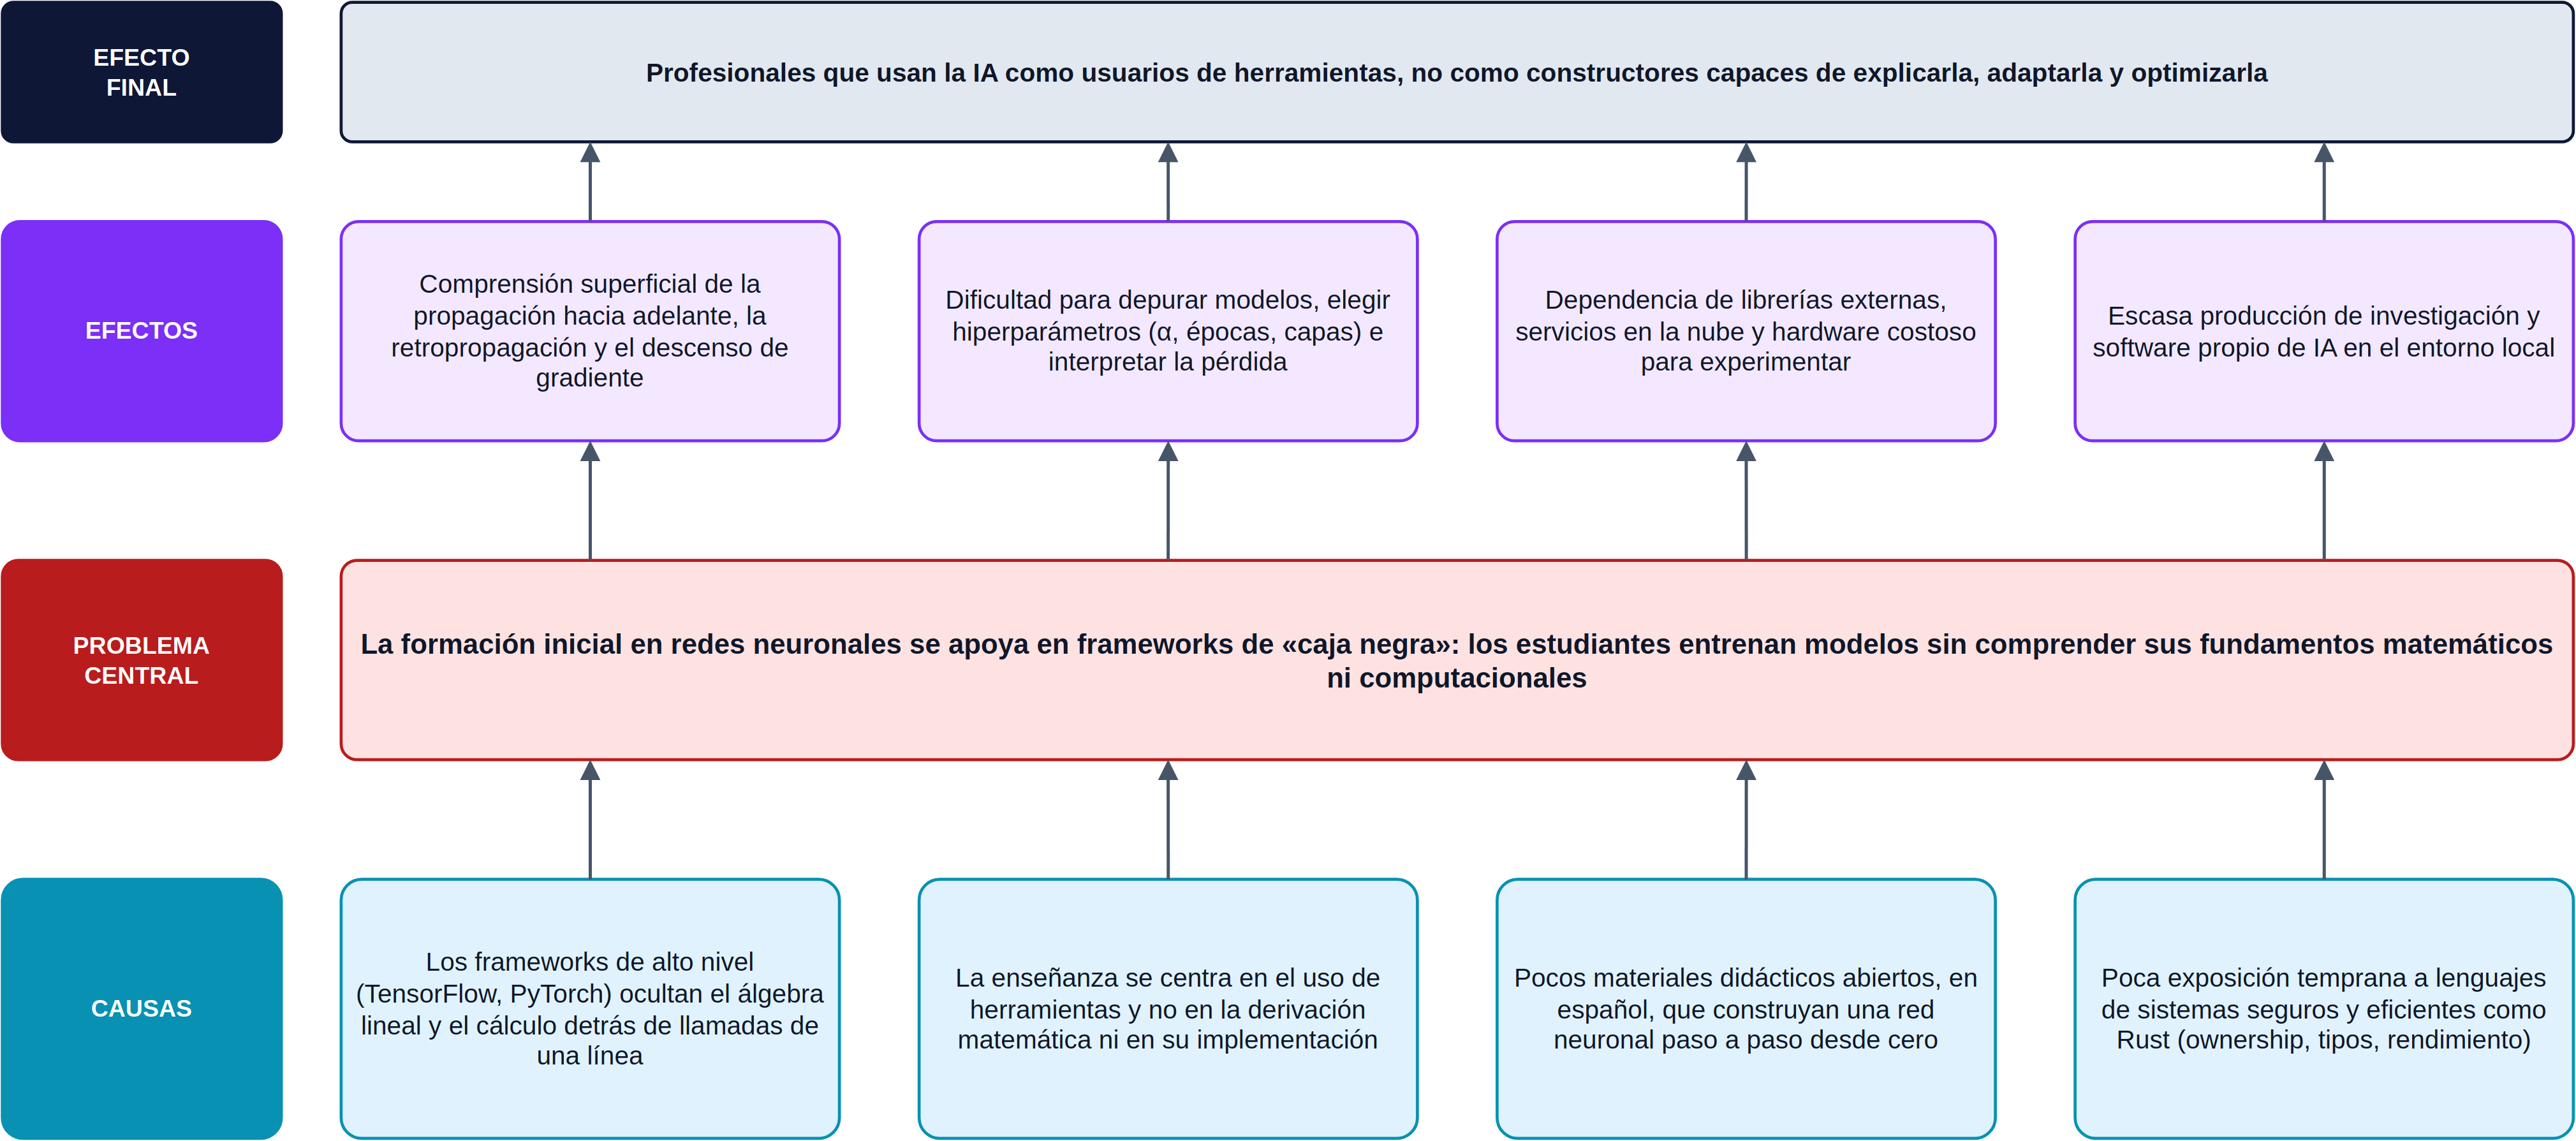
\includegraphics[width=\textwidth,height=0.62\textheight,keepaspectratio]{figuras/diag01_arbol_problemas.png}
\fuente{Las causas se ubican en la parte inferior, el problema central en el centro y los efectos y el efecto final en la parte superior. Diagrama editable: \texttt{diagramas/01\_arbol\_problemas.drawio}.}
\end{figure}

El análisis causal muestra cuatro factores que se refuerzan entre sí. En primer lugar, la enseñanza de la IA se apoya en bibliotecas que encapsulan el álgebra y el cálculo, de modo que el estudiante no necesita ---ni tiene oportunidad de--- implementar una multiplicación matricial o una derivada. En segundo lugar, la matemática de los primeros semestres se presenta de forma desconectada de sus aplicaciones computacionales, por lo que la regla de la cadena o el producto matriz-vector parecen contenidos abstractos sin relación con el software. En tercer lugar, los recursos disponibles suelen exigir equipos con alto poder de cómputo o servicios de pago. En cuarto lugar, las prácticas de programación de los primeros cursos rara vez incorporan pruebas automatizadas y experimentos reproducibles, lo que dificulta distinguir un programa que funciona de uno que parece funcionar. Como efecto, se forman usuarios de herramientas con escasa capacidad para explicar, depurar o adaptar los modelos que utilizan.

\subsection{Pregunta de investigación}
La formulación anterior se concreta en la siguiente pregunta, que guía el diseño de la solución y el análisis de resultados: ¿es posible construir, con fines educativos y sin \emph{frameworks} de aprendizaje automático, una red neuronal artificial en Rust capaz de aprender una relación lineal, clasificar valores booleanos y reconocer patrones visuales simples como las vocales A, E, I, O, U, verificando sus ecuaciones mediante pruebas automatizadas y experimentos reproducibles?

\subsection{Delimitación}
La delimitación establece las fronteras del trabajo para que los resultados se interpreten dentro de su alcance real. En el plano temático, el proyecto aborda redes neuronales densas de propagación hacia adelante (\emph{feedforward}) con funciones de activación Sigmoid, ReLU, lineal y softmax, pérdida de error cuadrático medio y descenso de gradiente. En el plano técnico, la implementación principal es el repositorio oficial del equipo (\url{\Repositorio}), escrito en Rust (edición 2024) sin crates de aprendizaje automático, y se ejecuta en un computador personal convencional. En el plano experimental, se desarrollan tres experimentos de complejidad progresiva ---$y=2x$, clasificación booleana y vocales--- con datos sintéticos definidos en el código fuente, complementados con XOR y vocales con ruido en el motor de validación. Quedan fuera del alcance las redes convolucionales y recurrentes, la aceleración por GPU, el procesamiento de conjuntos de datos masivos y el despliegue en producción.

\section{Justificación}\label{sec:justificacion}
La pertinencia del proyecto se sustenta en cuatro dimensiones complementarias: el valor técnico de la solución, su utilidad académica para la asignatura, su impacto social y educativo, y la viabilidad de su ejecución con los recursos disponibles.

\subsection{Justificación técnica}
Rust ofrece un rendimiento comparable al de C sin recolector de basura y con seguridad de memoria garantizada por el compilador \citep{klabnik2023,jung2018}. Su sistema de tipos y el manejo explícito de errores mediante \texttt{Result} permiten detectar de forma controlada los errores de dimensión que, en otros lenguajes, producirían resultados incorrectos silenciosos o fallos de segmentación. La herramienta \texttt{cargo} integra compilación, pruebas, análisis estático y documentación, lo que facilita una metodología de desarrollo verificable. Prescindir de dependencias externas obliga a implementar cada operación numérica, con la ventaja adicional de que el resultado es un binario pequeño, portable y auditable línea por línea.

\subsection{Justificación académica}
Construir una red neuronal desde cero obliga a traducir cada ecuación matemática en código verificable. Ese ejercicio consolida conocimientos de álgebra lineal (productos matriz-vector, transpuestas, producto de Hadamard), de cálculo diferencial (regla de la cadena y derivadas parciales) y de programación estructurada, y permite comprender por qué funcionan técnicas que en los \emph{frameworks} aparecen como una sola llamada a función \citep{nielsen2015,deisenroth2020}. Para Programación 1, el proyecto ofrece un caso integrador en el que variables, ciclos, funciones, arreglos, estructuras, módulos y pruebas cobran sentido dentro de un sistema completo, como se detalla en el Capítulo~\ref{cap:inf120}.

\subsection{Justificación social y educativa}
El proyecto se publica como código abierto y no requiere hardware especializado, licencias ni conexión permanente a servicios en la nube. Esto lo vuelve accesible para estudiantes de cualquier provincia y lo convierte en un material reutilizable para la enseñanza de la IA en la universidad pública. La prueba de escritorio documentada, las gráficas generadas desde datos reales y la guía de demostración permiten que otros estudiantes reproduzcan los resultados y los utilicen como punto de partida para sus propios proyectos.

\subsection{Viabilidad}
El proyecto es viable porque utiliza exclusivamente herramientas gratuitas (Rust, Cargo, Git, Python con \texttt{matplotlib}, \LaTeX{} y draw.io), se ejecuta en equipos convencionales y se apoya en una bibliografía consolidada. El equipo de cinco integrantes distribuyó el trabajo en fases con entregables verificables, y la validación mediante pruebas automatizadas y experimentos con semilla fija garantiza que cualquier evaluador pueda obtener los mismos resultados \citep{hernandez2018}.

\section{Objetivo general}\label{sec:objgeneral}
El objetivo general orienta la totalidad del proyecto y define el resultado verificable que se espera alcanzar.

\begin{nota}[Objetivo general]
Desarrollar una red neuronal artificial desde cero utilizando el lenguaje Rust, sin \emph{frameworks} de aprendizaje automático ni bibliotecas de álgebra lineal, implementando sus fundamentos matemáticos (álgebra lineal, funciones de activación, función de pérdida, gradientes y descenso de gradiente) y validando su funcionamiento mediante tres experimentos reproducibles y una verificación complementaria con pruebas automatizadas.
\end{nota}

\section{Objetivos específicos}\label{sec:objespecificos}
Los objetivos específicos descomponen el objetivo general en metas concretas y medibles, alineadas con las fases de desarrollo descritas en el Capítulo~\ref{cap:metodologia}. La Tabla~\ref{tab:objetivos} relaciona cada objetivo con su indicador de verificación.

\begin{enumerate}[label=\textbf{OE\arabic*.},leftmargin=3.2em,itemsep=4pt]
\item Implementar estructuras genéricas de vectores y matrices con operaciones de suma, resta, producto punto, multiplicación matricial, producto elemento a elemento, escalamiento y transpuesta, con validación de dimensiones.
\item Implementar las funciones de activación Sigmoid y ReLU, la función softmax, y la función de pérdida de error cuadrático medio (MSE) con su derivada.
\item Construir neuronas, capas densas y una red con propagación hacia adelante, y entrenarlas mediante gradientes y descenso de gradiente; extender la retropropagación a redes con capas ocultas en el motor complementario.
\item Verificar la corrección de las ecuaciones mediante pruebas unitarias, incluida la comparación entre gradientes analíticos y numéricos (\emph{gradient checking}).
\item Ejecutar y analizar tres experimentos progresivos ---regresión $y=2x$, clasificación booleana y reconocimiento de vocales A, E, I, O, U--- y complementarlos con XOR y vocales con ruido, registrando métricas reales en archivos CSV.
\item Medir el rendimiento real (tiempos de ejecución y tamaño del binario) compilado en modo \emph{release}.
\end{enumerate}

\begin{table}[!htbp]
\caption{Matriz de objetivos específicos, indicadores y medios de verificación}\label{tab:objetivos}
\small
\begin{tabularx}{\textwidth}{@{}l >{\raggedright}X >{\raggedright\arraybackslash}X@{}}
\toprule
Objetivo & Indicador verificable & Medio de verificación \\
\midrule
OE1 & Operaciones algebraicas con comprobación de dimensiones & \texttt{src/math/} (oficial) y pruebas de \texttt{math} (complementario) \\
OE2 & Activaciones, softmax y MSE operativas; derivadas verificadas & \texttt{src/neural/}, \texttt{src/learning/} y \emph{gradient checking} \\
OE3 & Neurona, capa y red entrenables; retropropagación multicapa & Experimentos oficiales y motor complementario \\
OE4 & 52 pruebas aprobadas en el motor complementario & Anexo~\ref{anx:tests} \\
OE5 & Métricas reales de los experimentos & \path{resultados/oficial/*.csv}, Capítulo~\ref{cap:implementacion} \\
OE6 & Tiempos de ejecución y tamaño del binario & \path{resultados/oficial/resumen.csv}, \path{benchmarks.csv} \\
\bottomrule
\end{tabularx}
\fuente{Elaboración propia. Los resultados de cada indicador se contrastan en el Capítulo~\ref{cap:conclusiones}.}
\end{table}

\chapter{Relación con la Asignatura Programación 1 (INF120)}\label{cap:inf120}
Este capítulo muestra que el proyecto no es un tema ajeno a la asignatura, sino una aplicación integradora de sus contenidos. Cada concepto de Programación 1 ---tipos de datos, estructuras de control, ciclos, funciones, arreglos, matrices, registros, modularidad, manejo de errores y entrada de argumentos--- aparece en el código fuente cumpliendo una función concreta dentro del sistema que aprende. La exposición sigue el orden habitual del programa de la asignatura y cada sección se ilustra con un fragmento extraído automáticamente del repositorio, de modo que el texto y el código no puedan divergir.

\section{Correspondencia entre contenidos y código}
La Tabla~\ref{tab:inf120} resume la correspondencia entre los contenidos de \Sigla{} y los elementos del proyecto. La columna central indica la construcción de Rust utilizada y la columna derecha, el lugar del código donde puede observarse.

\begin{table}[!htbp]
\caption{Correspondencia entre contenidos de Programación 1 y el código del proyecto}\label{tab:inf120}
\small
\begin{tabularx}{\textwidth}{@{}>{\raggedright}p{3.6cm} >{\raggedright}X >{\raggedright\arraybackslash}p{4.3cm}@{}}
\toprule
Contenido de \Sigla & Construcción en Rust & Ubicación en el proyecto \\
\midrule
Variables y tipos de datos & \texttt{f32}, \texttt{usize}, \texttt{char}, \texttt{\&str}; inmutabilidad por defecto y \texttt{let mut} & Todos los módulos \\
Operadores y expresiones & Aritméticos, relacionales, lógicos; \texttt{exp()}, \texttt{max} & \texttt{Activacion}, softmax \\
Estructuras condicionales & \texttt{if}/\texttt{else}, \texttt{match} con patrones & \texttt{main.rs}, \texttt{parse\_vowel} \\
Ciclos & \texttt{for} sobre rangos, \texttt{for} con \texttt{enumerate}, iteradores & Épocas y muestras de cada experimento \\
Funciones y parámetros & Paso por valor y por referencia (\texttt{\&}, \texttt{\&mut}) & \texttt{forward}, \texttt{update\_weights} \\
Arreglos y vectores & \texttt{Vec<T>}, rebanadas \texttt{\&[f32]}, arreglos fijos \texttt{[[\&str; 5]; 5]} & \texttt{Vector<T>}, patrones de vocales \\
Matrices & Almacenamiento por filas; patrones $5\times5$ aplanados & \texttt{Matrix<T>}, \texttt{encode} \\
Registros & \texttt{struct} con métodos en bloques \texttt{impl} & \texttt{Neuron}, \texttt{Layer}, \texttt{Network} \\
Genéricos & \texttt{Vector<T>} con restricciones de traits & \texttt{math/} \\
Modularidad & \texttt{mod}, \texttt{pub}, \texttt{use} & \texttt{math/}, \texttt{neural/}, \texttt{learning/}, \texttt{experiments/} \\
Validación y errores & \texttt{assert\_eq!}, \texttt{Result<T, E>}, \texttt{Option} & Dimensiones, vocal ingresada \\
Pruebas y depuración & Trazas por época, prueba de escritorio, \texttt{\#[test]} & Capítulo~\ref{cap:implementacion}, motor complementario \\
\bottomrule
\end{tabularx}
\fuente{Elaboración propia a partir del código fuente de \url{\Repositorio}.}
\end{table}

\section{Tipos de datos, variables y expresiones}
Toda la aritmética de la red del repositorio oficial se realiza con números de punto flotante de precisión simple (\texttt{f32}, IEEE~754), que representan unas siete cifras decimales significativas. Es una elección adecuada para una demostración: los tres experimentos alcanzan su objetivo, y el error final de la regresión $y=2x$ (\OfLinMseFin) se acerca al límite de esa precisión. Los índices y tamaños usan \texttt{usize}, el entero sin signo del tamaño de una dirección de memoria, y la vocal ingresada se maneja como \texttt{char}. En Rust las variables son inmutables por defecto; los pesos que cambian durante el entrenamiento se declaran con \texttt{let mut}, lo que hace visible en el código qué datos evolucionan.

\section{Funciones, parámetros y referencias}
Las operaciones matemáticas se implementan como funciones con parámetros tipados y valor de retorno explícito. El Código~\ref{cod:dot} muestra el producto punto genérico de \texttt{Vector<T>}: recibe el otro vector por referencia inmutable (\texttt{\&Vector<T>}), comprueba que las longitudes coincidan y acumula los productos con iteradores. Pasar por referencia evita copiar los datos, y el compilador garantiza que la función no los modifique.

\lstinputlisting[caption={Producto punto genérico con validación de longitudes (\texttt{src/math/vector.rs})},label=cod:dot]{generado/codigo/of_dot.rs}

\section{Estructuras de control}
El punto de entrada (Código~\ref{cod:main}) decide qué experimento ejecutar con un \texttt{match} sobre el primer argumento de la línea de comandos. A diferencia de un \texttt{switch} tradicional, el compilador exige que \texttt{match} cubra todos los casos posibles; el comodín \texttt{Some(value)} trata cualquier otro texto como una vocal y \texttt{None}, la ausencia de argumentos.

\lstinputlisting[caption={Selección del experimento con \texttt{match} (\texttt{src/main.rs})},label=cod:main]{generado/codigo/of_main.rs}

El Código~\ref{cod:argmax} busca el índice del valor máximo, operación que convierte las cinco probabilidades de la red de vocales en una clase. El algoritmo es el clásico de Programación 1, expresado con iteradores: recorre los pares (índice, valor) y conserva el mayor.

\lstinputlisting[caption={Búsqueda del índice máximo (\texttt{src/experiments/vowels.rs})},label=cod:argmax]{generado/codigo/of_argmax.rs}

\section{Ciclos}
El entrenamiento es un conjunto de ciclos anidados: un ciclo externo sobre las épocas y un ciclo interno sobre las muestras. En el experimento $y=2x$ (Código~\ref{cod:of-lin}, Capítulo~\ref{cap:implementacion}) el ciclo externo \texttt{for epoch in 1..=max\_epochs} se interrumpe con \texttt{break} cuando el error alcanza la meta, y el interno acumula los gradientes. El mismo patrón, con \texttt{enumerate} para conocer el índice de cada muestra, aparece en los experimentos booleano y de vocales.

\section{Arreglos, vectores y matrices}
La estructura \texttt{Vector<T>} encapsula un arreglo dinámico \texttt{Vec<T>}, y \texttt{Matrix<T>} almacena sus $m\times n$ elementos en un único arreglo contiguo en orden por filas: el elemento de la fila $i$ y columna $j$ ocupa la posición $i\cdot n+j$. El Código~\ref{cod:mulvec} muestra la multiplicación de matrices con tres ciclos anidados, la implementación directa de $c_{ij}=\sum_k a_{ik}b_{kj}$.

\lstinputlisting[caption={Multiplicación de matrices sobre almacenamiento por filas (\texttt{src/math/matrix.rs})},label=cod:mulvec]{generado/codigo/of_multiply.rs}

Los arreglos de tamaño fijo también aparecen en el proyecto. Las cinco vocales se dibujan en un arreglo \texttt{[[\&str; 5]; 5]}, donde \texttt{\#} representa un píxel encendido (Código~\ref{cod:patrones}). La función \texttt{encode} (Código~\ref{cod:encode}) recorre la matriz fila por fila y la aplana en un vector de 25 valores 0 o 1: el mismo recorrido por filas que se enseña para matrices en la asignatura.

\lstinputlisting[caption={Patrones binarios $5\times5$ de las vocales (\texttt{src/experiments/vowels.rs})},label=cod:patrones]{generado/codigo/of_patrones.rs}
\lstinputlisting[caption={Aplanado de un patrón en 25 entradas (\texttt{src/experiments/vowels.rs})},label=cod:encode]{generado/codigo/of_encode.rs}

\section{Registros y procedimientos}
Los registros de Programación 1 se corresponden con las estructuras (\texttt{struct}) de Rust, y los procedimientos que operan sobre ellos, con los métodos de los bloques \texttt{impl}. La neurona (Código~\ref{cod:neuron-struct}) es un registro con dos campos privados, sus pesos y su bias; el exterior solo puede usarla mediante sus métodos públicos \texttt{new} y \texttt{forward}, lo que aplica el principio de encapsulamiento.

\lstinputlisting[caption={Registro de una neurona (\texttt{src/neural/neuron.rs})},label=cod:neuron-struct]{generado/codigo/of_neuron_struct.rs}

\section{Validación de datos y manejo de errores}
Un error frecuente en los primeros cursos es combinar arreglos de tamaños distintos. El repositorio oficial lo previene con \texttt{assert\_eq!}: si las dimensiones no coinciden, el programa se detiene con un mensaje que describe la causa, en lugar de producir un resultado incorrecto. Para los datos ingresados por el usuario utiliza \texttt{Result} (Código~\ref{cod:parsear}): la vocal se normaliza a mayúscula y, si no es A, E, I, O o U, se devuelve un error que el programa informa sin interrumpirse de forma abrupta.

\lstinputlisting[caption={Validación de la vocal ingresada (\texttt{src/experiments/vowels.rs})},label=cod:parsear]{generado/codigo/of_parse.rs}

\section{Pruebas, depuración y prueba de escritorio}
La prueba de escritorio, técnica clásica de Programación 1 para seguir manualmente un algoritmo, se aplica en dos niveles. El repositorio oficial imprime en cada época los gradientes y los parámetros, de modo que cada actualización puede comprobarse con calculadora (Tabla~\ref{tab:of-bool}); el motor complementario registra además las primeras iteraciones del entrenamiento (Sección~\ref{sec:escritorio}) e incluye 52 pruebas automatizadas con \texttt{\#[test]} y \texttt{assert!}. Así, verificar un programa se muestra como parte de su construcción.

\begin{nota}[Propuesta de uso en aula]
En \Sigla, los estudiantes pueden reproducir la prueba de escritorio, modificar la tasa de aprendizaje o las épocas, dibujar una nueva letra en los patrones o añadir una función a \texttt{Activacion} con su prueba \texttt{\#[test]}.
\end{nota}

\chapter{Marco Teórico}\label{cap:marco}
El marco teórico reúne los fundamentos matemáticos que sustentan el funcionamiento de una red neuronal artificial y los fundamentos técnicos del lenguaje Rust que justifican su elección. El capítulo avanza desde los objetos elementales ---vectores y matrices--- hasta el algoritmo completo de entrenamiento, y cada ecuación numerada tiene una implementación directa en el código fuente del proyecto, indicada en el texto para facilitar la trazabilidad entre la teoría y la práctica.

\section{Fundamentos de álgebra lineal}
El álgebra lineal proporciona el lenguaje con el que se describen los datos y las transformaciones de una red neuronal. Una entrada se representa como un vector, los parámetros de una capa como una matriz y un vector, y el procesamiento de la capa como una transformación afín seguida de una función no lineal \citep{strang2016,deisenroth2020}.

\subsection{Vectores y matrices}
Un vector $\mathbf{x}\in\mathbb{R}^{n}$ es una lista ordenada de $n$ números reales, interpretada en este trabajo como vector columna. Una matriz $\mathbf{W}\in\mathbb{R}^{m\times n}$ es un arreglo rectangular de $m$ filas y $n$ columnas \citep{strang2016}. En la implementación, las matrices se almacenan en un único arreglo contiguo en orden por filas (\emph{row-major}), de modo que el elemento $w_{ij}$ ocupa la posición $i\cdot n + j$ (con índices desde cero). La estructura \texttt{Vector} de \texttt{src/math/vector.rs} y la estructura \texttt{Matrix} de \texttt{src/math/matrix.rs} materializan estas definiciones.

\subsection{Operaciones fundamentales}
Sean $\mathbf{x},\mathbf{y}\in\mathbb{R}^{n}$, $\mathbf{A}\in\mathbb{R}^{m\times k}$ y $\mathbf{B}\in\mathbb{R}^{k\times n}$. Las operaciones implementadas, con su complejidad temporal, son:
\begin{align}
\mathbf{x}\cdot\mathbf{y} &= \sum_{i=1}^{n} x_i y_i, &&\text{(producto punto, } O(n)\text{)}\label{eq:dot}\\
(\mathbf{A}\mathbf{B})_{ij} &= \sum_{l=1}^{k} a_{il}\, b_{lj}, &&\text{(producto matricial, } O(mkn)\text{)}\label{eq:matmul}\\
(\mathbf{x}\odot\mathbf{y})_i &= x_i\, y_i, &&\text{(producto de Hadamard, } O(n)\text{)}\label{eq:hadamard}\\
(\mathbf{A}^{\top})_{ij} &= a_{ji}, &&\text{(transpuesta, } O(mk)\text{)}\label{eq:transpuesta}\\
(\mathbf{x}\,\mathbf{y}^{\top})_{ij} &= x_i\, y_j. &&\text{(producto exterior, } O(n^2)\text{)}\label{eq:outer}
\end{align}
Estas operaciones solo están definidas cuando las dimensiones son compatibles; por ejemplo, el producto $\mathbf{A}\mathbf{B}$ exige que el número de columnas de $\mathbf{A}$ coincida con el número de filas de $\mathbf{B}$. En el proyecto, toda violación de dimensiones produce un error explícito en lugar de un resultado incorrecto.

\subsection{Interpretación geométrica}
El producto punto mide la alineación entre dos vectores: $\mathbf{w}\cdot\mathbf{x} = \lVert\mathbf{w}\rVert\,\lVert\mathbf{x}\rVert\cos\theta$. En consecuencia, el conjunto de puntos que satisface $\mathbf{w}\cdot\mathbf{x} + b = 0$ es un hiperplano con vector normal $\mathbf{w}$, que divide el espacio de entradas en dos semiespacios. El producto matriz-vector $\mathbf{W}\mathbf{x}$ calcula simultáneamente $m$ productos punto, uno por fila, y por ello describe de forma compacta el trabajo de $m$ neuronas que reciben la misma entrada. El producto exterior $\mathbf{u}\mathbf{v}^{\top}$, en cambio, produce una matriz de rango uno y aparece de forma natural al calcular el gradiente de los pesos de una capa (Ecuación~\eqref{eq:gradW}). La operación $\mathbf{W}^{\top}\mathbf{v}$ se implementa sin construir explícitamente la transpuesta, recorriendo la matriz por columnas, lo que ahorra memoria en la retropropagación.

\section{La neurona artificial}
La neurona artificial, inspirada en el modelo de \citet{mcculloch1943} y en el perceptrón de \citet{rosenblatt1958}, recibe un vector de entradas $\mathbf{x}\in\mathbb{R}^{n}$, lo combina linealmente con un vector de pesos $\mathbf{w}\in\mathbb{R}^{n}$ y un sesgo $b\in\mathbb{R}$, y aplica una función de activación $f$:
\begin{equation}
z = \mathbf{w}\cdot\mathbf{x} + b = \sum_{i=1}^{n} w_i x_i + b, \qquad a = f(z).\label{eq:neurona}
\end{equation}
La suma ponderada $z$ define un hiperplano en el espacio de entradas. Por ello, una única neurona solo puede separar clases que sean linealmente separables, limitación que \citet{minsky1969} formalizaron con el ejemplo de la compuerta XOR. Para XOR, una neurona con salida $a = f(w_1x_1 + w_2x_2 + b)$ y umbral en $z=0$ necesitaría simultáneamente $b<0$ (para $(0,0)\mapsto 0$), $w_1+b>0$ y $w_2+b>0$ (para $(1,0)$ y $(0,1)\mapsto 1$) y $w_1+w_2+b<0$ (para $(1,1)\mapsto 0$). Sumando las dos desigualdades intermedias se obtiene $w_1+w_2+2b>0$, es decir, $w_1+w_2+b>-b>0$, lo que contradice la última condición. La contradicción demuestra que ningún conjunto de parámetros resuelve el problema con una sola neurona, resultado que se observa experimentalmente en la Sección~\ref{sec:exp2}.

\section{Funciones de activación}
Las funciones de activación introducen no linealidad; sin ellas, la composición de varias capas seguiría siendo una transformación lineal, pues $\mathbf{W}_2(\mathbf{W}_1\mathbf{x}+\mathbf{b}_1)+\mathbf{b}_2 = (\mathbf{W}_2\mathbf{W}_1)\mathbf{x} + (\mathbf{W}_2\mathbf{b}_1+\mathbf{b}_2)$ \citep{goodfellow2016}. La Figura~\ref{fig:activaciones} muestra las dos funciones no lineales implementadas y sus derivadas.

\begin{figure}[!htbp]
\caption{Funciones de activación Sigmoid y ReLU con sus derivadas}\label{fig:activaciones}
\centering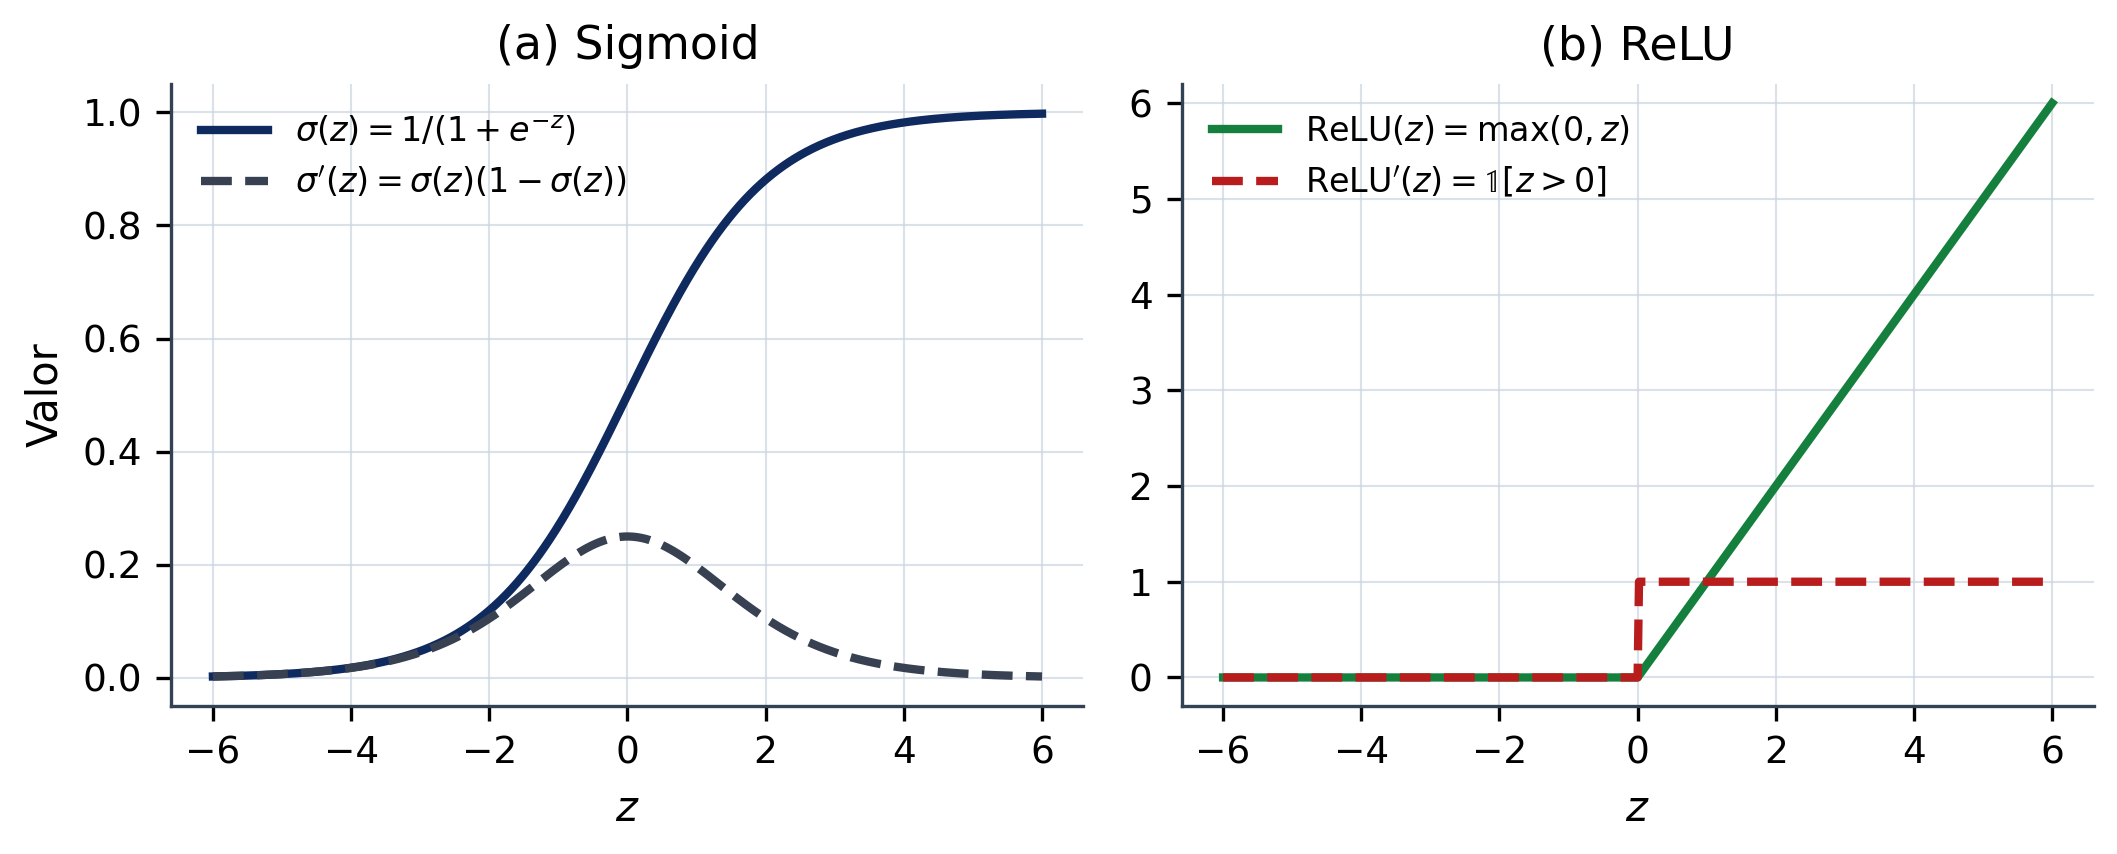
\includegraphics[width=\textwidth]{figuras/fig01_activaciones.png}
\fuente{(a) Sigmoid y su derivada, con máximo $0.25$ en $z=0$. (b) ReLU y su derivada escalón. Curvas trazadas con las Ecuaciones~\eqref{eq:sigmoid} y~\eqref{eq:relu}, idénticas a las implementadas en \texttt{src/nn/activation.rs}.}
\end{figure}

\subsection{Función Sigmoid}
La función logística o Sigmoid transforma cualquier número real en un valor del intervalo $(0,1)$, por lo que su salida puede interpretarse como una probabilidad o un grado de activación:
\begin{equation}
\sigma(z) = \frac{1}{1+e^{-z}}, \qquad \sigma'(z) = \sigma(z)\,\bigl(1-\sigma(z)\bigr).\label{eq:sigmoid}
\end{equation}
La derivada se obtiene aplicando la regla del cociente:
\begin{equation*}
\sigma'(z) = \frac{e^{-z}}{(1+e^{-z})^2} = \frac{1}{1+e^{-z}}\cdot\frac{e^{-z}}{1+e^{-z}} = \frac{1}{1+e^{-z}}\cdot\Bigl(1-\frac{1}{1+e^{-z}}\Bigr) = \sigma(z)\bigl(1-\sigma(z)\bigr).
\end{equation*}
Su valor máximo es $0.25$ en $z=0$, y tiende a cero cuando $|z|$ crece. Esta saturación explica la lentitud del aprendizaje cuando las neuronas reciben entradas de gran magnitud y, en redes profundas, el desvanecimiento del gradiente, pues el producto de muchas derivadas menores o iguales a $0.25$ decrece exponencialmente con la profundidad \citep{lecun1998}. Para evitar desbordamientos numéricos al evaluar $e^{-z}$ con $z$ muy negativo, la implementación usa la forma equivalente $\sigma(z) = e^{z}/(1+e^{z})$ cuando $z<0$.

\subsection{Función ReLU}
La unidad lineal rectificada (ReLU) anula los valores negativos y conserva los positivos:
\begin{equation}
\mathrm{ReLU}(z) = \max(0, z), \qquad \mathrm{ReLU}'(z) = \begin{cases}1 & z>0\\ 0 & z\le 0\end{cases}\label{eq:relu}
\end{equation}
ReLU es computacionalmente económica, no se satura para entradas positivas y mitiga el desvanecimiento del gradiente en redes profundas \citep{glorot2010,he2015}. En $z=0$ la derivada no existe; por convención se adopta el valor $0$. Su principal inconveniente es que una neurona cuya entrada permanece negativa deja de aprender, fenómeno conocido como neurona muerta.

\subsection{Función lineal}
Para problemas de regresión se utiliza la identidad $f(z)=z$, cuya derivada es $f'(z)=1$. Una red con una única neurona lineal y pérdida MSE equivale a una regresión lineal por mínimos cuadrados resuelta iterativamente, lo que hace del Experimento~1 un caso de prueba con solución analítica conocida.

\section{Función de pérdida: error cuadrático medio}
La función de pérdida cuantifica la discrepancia entre la predicción de la red y el valor esperado, y es la magnitud que el entrenamiento minimiza. Dado un vector de predicciones $\hat{\mathbf{y}}\in\mathbb{R}^{n}$ y un vector objetivo $\mathbf{y}\in\mathbb{R}^{n}$, el error cuadrático medio y su gradiente son:
\begin{equation}
\mathcal{L}(\hat{\mathbf{y}},\mathbf{y}) = \frac{1}{n}\sum_{i=1}^{n}(\hat{y}_i - y_i)^2, \qquad \frac{\partial\mathcal{L}}{\partial \hat{y}_i} = \frac{2}{n}(\hat{y}_i - y_i).\label{eq:mse}
\end{equation}
El MSE es siempre no negativo, vale cero únicamente cuando la predicción coincide exactamente con el objetivo y penaliza con mayor peso los errores grandes debido al término cuadrático \citep{bishop2006}. Desde la perspectiva estadística, minimizar el MSE equivale a maximizar la verosimilitud bajo la hipótesis de ruido gaussiano. En el Experimento~2, un MSE de $0.25$ corresponde a predecir $0.5$ para todas las entradas de XOR, valor de referencia útil para interpretar el estancamiento del perceptrón.

\section{Red neuronal multicapa}
Una red multicapa (\emph{multilayer perceptron}) organiza las neuronas en $L$ capas densas, en las que cada neurona de una capa recibe todas las salidas de la capa anterior. Para la capa $l$ con $n_{l-1}$ entradas y $n_l$ neuronas, los parámetros son la matriz $\mathbf{W}^{(l)}\in\mathbb{R}^{n_l\times n_{l-1}}$ y el vector $\mathbf{b}^{(l)}\in\mathbb{R}^{n_l}$, de modo que la capa tiene $n_l(n_{l-1}+1)$ parámetros. La propagación hacia adelante es:
\begin{equation}
\mathbf{z}^{(l)} = \mathbf{W}^{(l)}\mathbf{a}^{(l-1)} + \mathbf{b}^{(l)}, \qquad \mathbf{a}^{(l)} = f^{(l)}\bigl(\mathbf{z}^{(l)}\bigr), \qquad \mathbf{a}^{(0)} = \mathbf{x}.\label{eq:forward}
\end{equation}
Aplicando esta fórmula, la red 2-4-1 del Experimento~2 tiene $4\cdot(2+1) + 1\cdot(4+1) = 17$ parámetros, y la red 25-10-5 del Experimento~3 tiene $10\cdot 26 + 5\cdot 11 = 315$. El teorema de aproximación universal garantiza que una red con una sola capa oculta y un número suficiente de neuronas con activación sigmoidal puede aproximar cualquier función continua en un dominio compacto con precisión arbitraria \citep{cybenko1989,hornik1989}. El teorema asegura la existencia de los parámetros, pero no indica cómo encontrarlos; esa tarea corresponde al algoritmo de entrenamiento.

\section{Retropropagación del error}
La retropropagación (\emph{backpropagation}) calcula eficientemente el gradiente de la pérdida respecto a todos los parámetros aplicando la regla de la cadena desde la salida hacia la entrada \citep{rumelhart1986}. Se define el error local de la capa $l$ como $\boldsymbol{\delta}^{(l)} = \partial\mathcal{L}/\partial\mathbf{z}^{(l)}$, es decir, la sensibilidad de la pérdida respecto a la suma ponderada de cada neurona.

\subsection{Regla de la cadena}
Si $\mathcal{L}$ depende de $z$ a través de una cadena de funciones $z\mapsto a\mapsto \mathcal{L}$, la regla de la cadena establece que $\frac{d\mathcal{L}}{dz} = \frac{d\mathcal{L}}{da}\cdot\frac{da}{dz}$. Cuando una variable influye en la pérdida a través de varios caminos, las contribuciones se suman: $\frac{\partial\mathcal{L}}{\partial a_j} = \sum_k \frac{\partial\mathcal{L}}{\partial z_k}\frac{\partial z_k}{\partial a_j}$. Estas dos reglas son suficientes para derivar todo el algoritmo.

\subsection{Derivación paso a paso}
Para la capa de salida $L$, por la regla de la cadena:
\begin{equation}
\delta_j^{(L)} = \frac{\partial\mathcal{L}}{\partial a_j^{(L)}}\cdot\frac{\partial a_j^{(L)}}{\partial z_j^{(L)}} = \frac{2}{n_L}\bigl(a_j^{(L)}-y_j\bigr)\, f'\bigl(z_j^{(L)}\bigr)
\;\Longrightarrow\; \boldsymbol{\delta}^{(L)} = \nabla_{\mathbf{a}}\mathcal{L}\odot f'\bigl(\mathbf{z}^{(L)}\bigr).\label{eq:deltaL}
\end{equation}
Para una capa oculta $l$, cada $z_j^{(l)}$ influye en la pérdida a través de todas las neuronas $k$ de la capa siguiente:
\begin{equation}
\begin{split}
\delta_j^{(l)} &= \sum_{k}\frac{\partial\mathcal{L}}{\partial z_k^{(l+1)}}\frac{\partial z_k^{(l+1)}}{\partial a_j^{(l)}}\frac{\partial a_j^{(l)}}{\partial z_j^{(l)}} = \Bigl(\sum_k w_{kj}^{(l+1)}\delta_k^{(l+1)}\Bigr) f'\bigl(z_j^{(l)}\bigr)\\
\Longrightarrow\quad \boldsymbol{\delta}^{(l)} &= \bigl(\mathbf{W}^{(l+1)\top}\boldsymbol{\delta}^{(l+1)}\bigr)\odot f'\bigl(\mathbf{z}^{(l)}\bigr).
\end{split}\label{eq:deltal}
\end{equation}
Como $z_j^{(l)} = \sum_i w_{ji}^{(l)}a_i^{(l-1)} + b_j^{(l)}$, se cumple $\partial z_j^{(l)}/\partial w_{ji}^{(l)} = a_i^{(l-1)}$ y $\partial z_j^{(l)}/\partial b_j^{(l)} = 1$, de modo que los gradientes de los parámetros resultan:
\begin{equation}
\frac{\partial\mathcal{L}}{\partial\mathbf{W}^{(l)}} = \boldsymbol{\delta}^{(l)}\,\mathbf{a}^{(l-1)\top}, \qquad \frac{\partial\mathcal{L}}{\partial\mathbf{b}^{(l)}} = \boldsymbol{\delta}^{(l)}.\label{eq:gradW}
\end{equation}
El costo de la retropropagación es del mismo orden que el de la propagación hacia adelante, $O(P)$, donde $P$ es el número total de parámetros, lo que la hace mucho más eficiente que estimar cada derivada por separado, cuyo costo sería $O(P^2)$ \citep{baydin2018}. En la implementación, cada capa guarda en caché su entrada $\mathbf{a}^{(l-1)}$ y su suma ponderada $\mathbf{z}^{(l)}$ durante la propagación hacia adelante, y el método \texttt{Layer::backward} aplica literalmente las Ecuaciones~\eqref{eq:deltal} y~\eqref{eq:gradW}.

\section{Descenso de gradiente}
El descenso de gradiente actualiza cada parámetro en dirección opuesta al gradiente, que es la dirección de máximo crecimiento local de la pérdida, con una tasa de aprendizaje $\alpha>0$:
\begin{equation}
\mathbf{W}^{(l)} \leftarrow \mathbf{W}^{(l)} - \alpha\,\frac{\partial\mathcal{L}}{\partial\mathbf{W}^{(l)}}, \qquad \mathbf{b}^{(l)} \leftarrow \mathbf{b}^{(l)} - \alpha\,\frac{\partial\mathcal{L}}{\partial\mathbf{b}^{(l)}}.\label{eq:gd}
\end{equation}
La justificación proviene de la aproximación de Taylor de primer orden: para un desplazamiento pequeño $\Delta\boldsymbol{\theta} = -\alpha\nabla\mathcal{L}$, se tiene $\mathcal{L}(\boldsymbol{\theta}+\Delta\boldsymbol{\theta}) \approx \mathcal{L}(\boldsymbol{\theta}) - \alpha\lVert\nabla\mathcal{L}\rVert^2 \le \mathcal{L}(\boldsymbol{\theta})$. En la variante estocástica (SGD) utilizada en este proyecto, la actualización se realiza después de cada muestra, lo que introduce ruido en la trayectoria pero permite avanzar sin recorrer todo el conjunto de datos \citep{bottou2010}. Una tasa $\alpha$ muy pequeña produce un aprendizaje extremadamente lento; una tasa excesiva provoca oscilaciones, divergencia o saturación de las neuronas \citep{ruder2016}. Este comportamiento se verifica experimentalmente en la Sección~\ref{sec:exp2}.

\section{Inicialización de pesos}
Si todos los pesos se inicializan con el mismo valor, las neuronas de una capa reciben gradientes idénticos y nunca se diferencian, problema conocido como simetría. Si se inicializan con valores demasiado grandes, las neuronas Sigmoid se saturan desde el inicio; si son demasiado pequeños, la señal se atenúa al atravesar las capas. Por ello se emplea inicialización aleatoria uniforme en $[-\ell,\ell]$ con la regla de \citet{glorot2010} para Sigmoid y lineal, y la de \citet{he2015} para ReLU:
\begin{equation}
\ell_{\text{Xavier}} = \sqrt{\frac{6}{n_{\text{in}}+n_{\text{out}}}}, \qquad \ell_{\text{He}} = \sqrt{\frac{6}{n_{\text{in}}}}.\label{eq:init}
\end{equation}
Ambas reglas buscan que la varianza de las activaciones y de los gradientes se mantenga aproximadamente constante entre capas. Los sesgos se inicializan en cero, pues la asimetría ya la aportan los pesos.

\section{Verificación numérica de gradientes}
Una implementación incorrecta de la retropropagación puede producir una red que aprende parcialmente y ocultar el error. Para comprobar que las derivadas analíticas están correctamente implementadas, se compara cada componente del gradiente con su aproximación por diferencias centrales \citep{lecun1998,goodfellow2016}:
\begin{equation}
\frac{\partial\mathcal{L}}{\partial\theta} \approx \frac{\mathcal{L}(\theta+\varepsilon)-\mathcal{L}(\theta-\varepsilon)}{2\varepsilon}, \qquad \text{error relativo} = \frac{|g_{\text{num}}-g_{\text{ana}}|}{\max(|g_{\text{num}}|+|g_{\text{ana}}|,\,10^{-12})}.\label{eq:gradcheck}
\end{equation}
Desarrollando $\mathcal{L}(\theta\pm\varepsilon)$ en serie de Taylor, los términos de orden par se cancelan y el error de truncamiento resulta $O(\varepsilon^{2})$, frente a $O(\varepsilon)$ de la diferencia hacia adelante. Por ello, un error relativo muy pequeño indica que la retropropagación es correcta. El proyecto aplica esta verificación a todos los parámetros de redes 2-4-1, 3-5-4-2 y 25-10-5.

\section{Métricas de evaluación}
Para regresión se utiliza el propio MSE. Para clasificación se utiliza la exactitud (\emph{accuracy}), definida como la proporción de muestras correctamente clasificadas, y la matriz de confusión $\mathbf{C}\in\mathbb{N}^{K\times K}$, cuyo elemento $c_{ij}$ cuenta las muestras de clase real $i$ predichas como clase $j$:
\begin{equation}
\text{exactitud} = \frac{\sum_{i=1}^{K} c_{ii}}{\sum_{i=1}^{K}\sum_{j=1}^{K} c_{ij}}.\label{eq:accuracy}
\end{equation}
En clasificación binaria (XOR) se asigna la clase 1 cuando la salida es mayor o igual que $0.5$. En clasificación multiclase con codificación \emph{one-hot}, la clase predicha es $\hat{k} = \arg\max_k \hat{y}_k$ \citep{bishop2006}. La matriz de confusión complementa la exactitud porque revela qué clases se confunden entre sí, información que la exactitud global oculta.

\section{Fundamentos técnicos de Rust}
Rust es un lenguaje de programación de sistemas compilado, con tipado estático y fuerte, diseñado para ofrecer seguridad de memoria sin recolector de basura \citep{klabnik2023,matsakis2014}. Las siguientes subsecciones describen las características del lenguaje que intervienen directamente en el diseño del motor.

\subsection{Propiedad, préstamos y tiempos de vida}
El modelo de propiedad (\emph{ownership}) establece que cada valor tiene un único dueño y se libera automáticamente cuando su dueño sale de ámbito. Los préstamos (\emph{borrowing}) permiten referencias inmutables múltiples (\texttt{\&T}) o una única referencia mutable (\texttt{\&mut T}), lo que elimina en tiempo de compilación las carreras de datos y los accesos a memoria liberada \citep{blandy2021}. \citet{jung2018} demostraron formalmente la solidez de estas garantías en el proyecto RustBelt. La Figura~\ref{fig:memoria} muestra cómo se aplican estas reglas en el motor: la red posee sus capas, cada capa posee sus matrices y vectores en el montón, y las funciones de cálculo reciben referencias prestadas.

\begin{figure}[!htbp]
\caption{Modelo de memoria, propiedad y préstamos en el motor}\label{fig:memoria}
\centering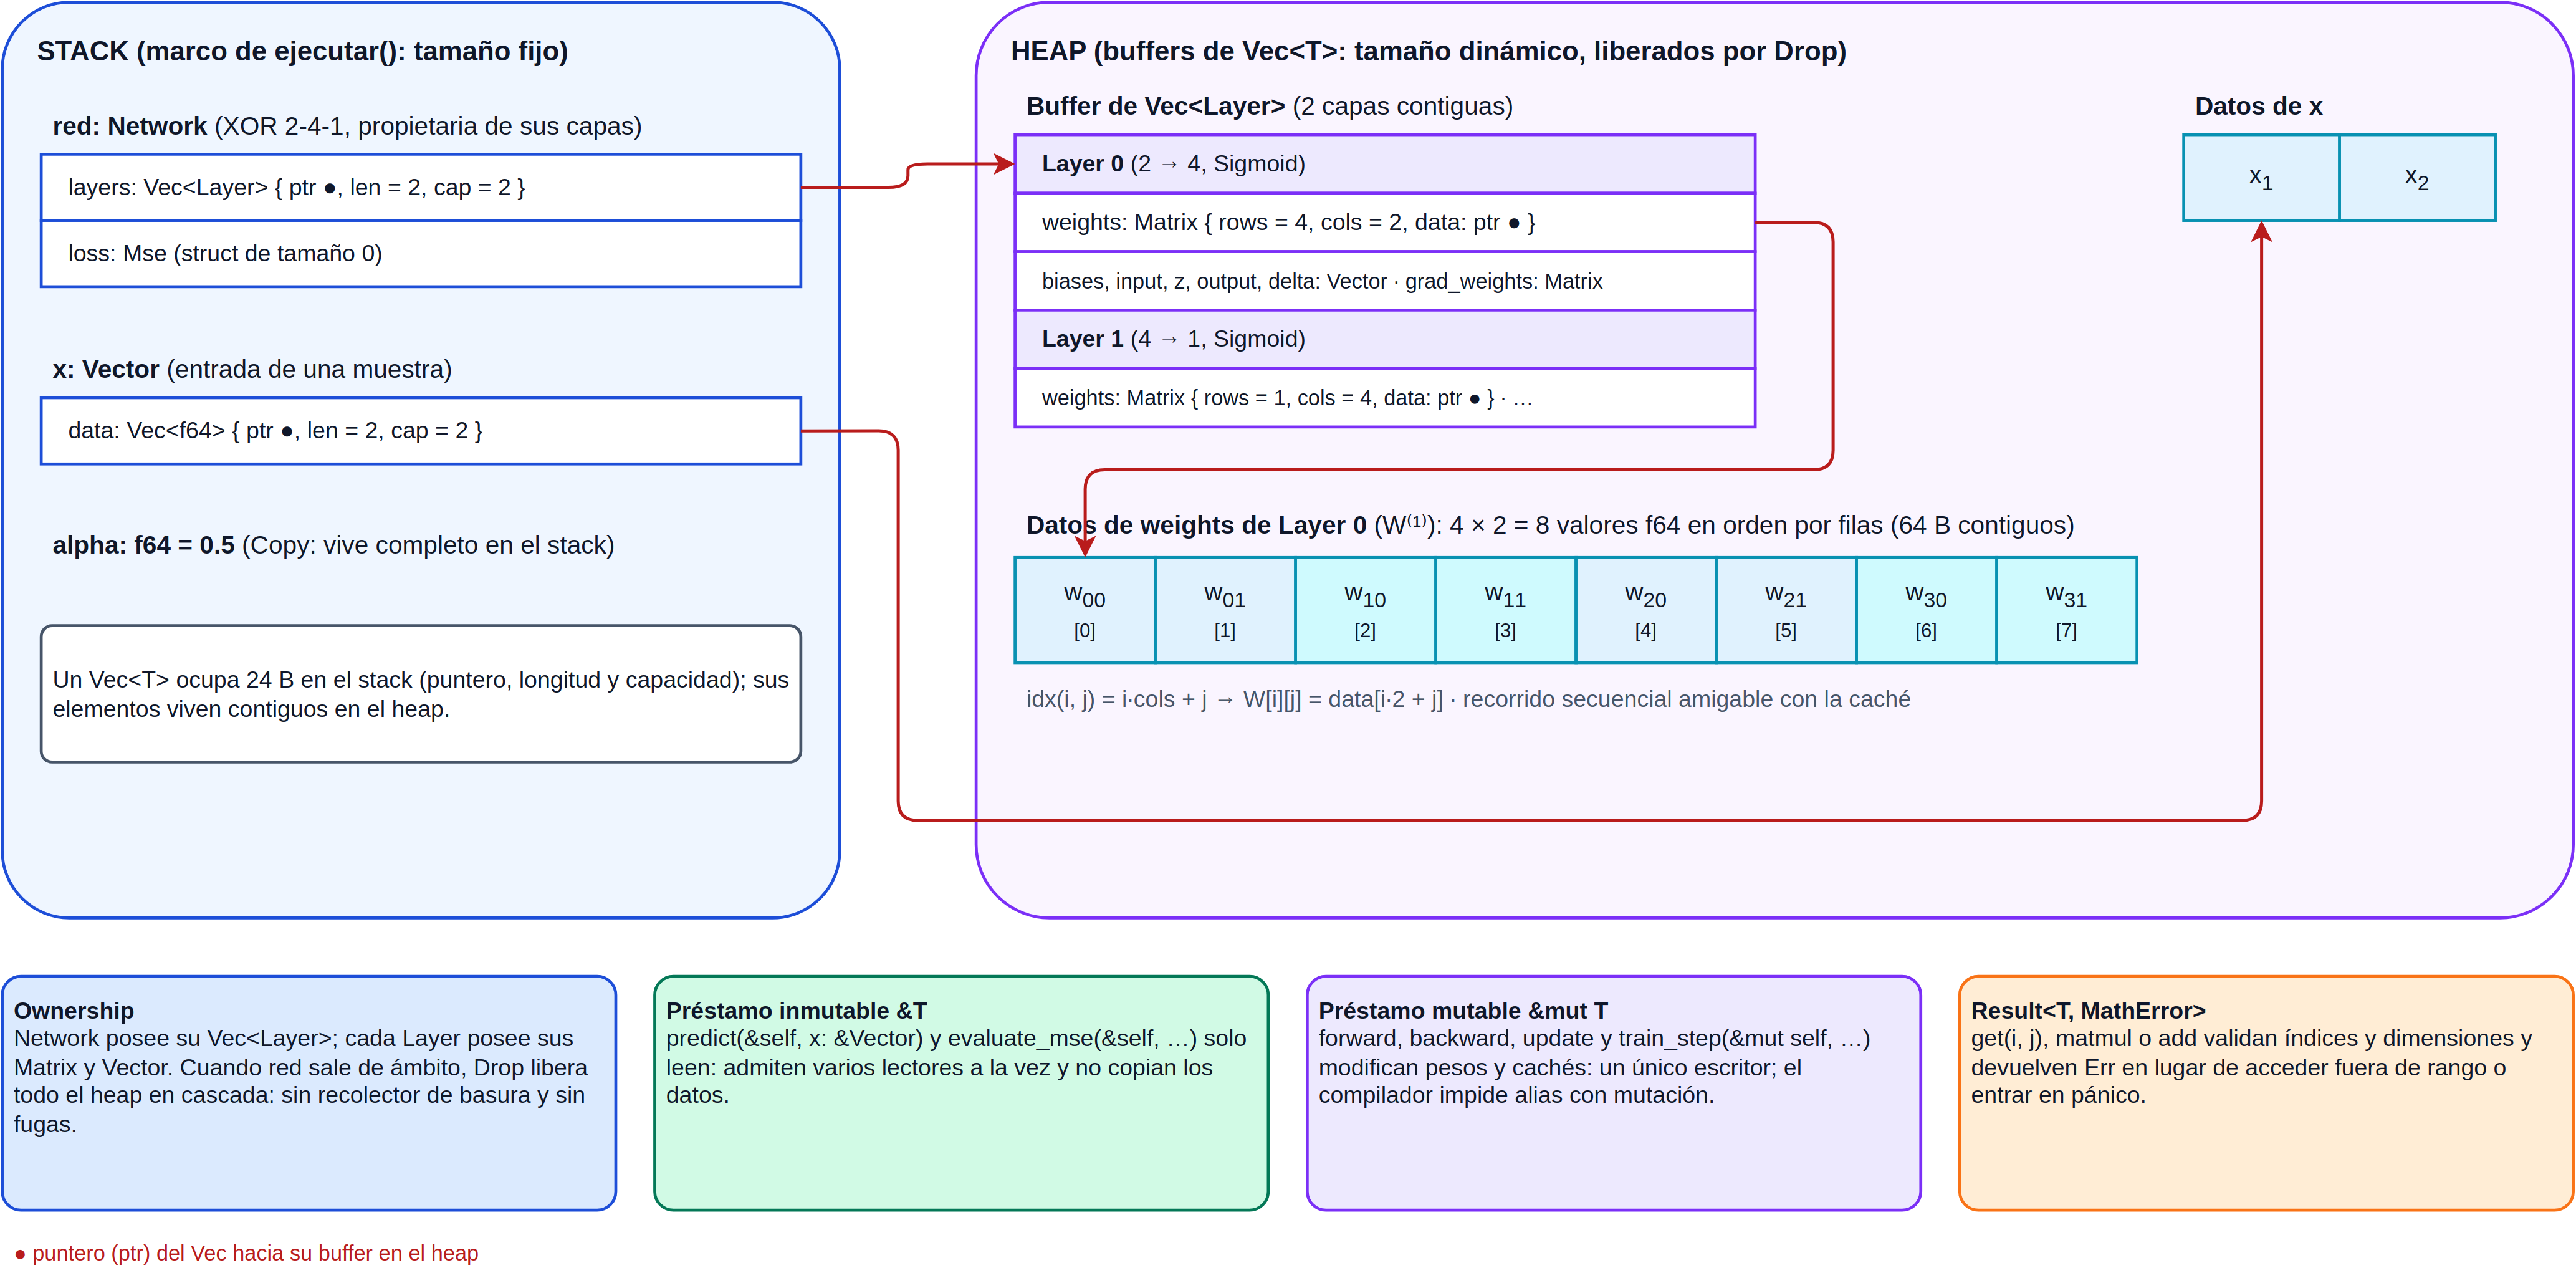
\includegraphics[width=\textwidth,height=0.55\textheight,keepaspectratio]{figuras/diag04_memoria_rust.png}
\fuente{La pila contiene las estructuras de control y el montón los arreglos de datos de cada capa. Diagrama editable: \texttt{diagramas/04\_memoria\_ownership\_rust.drawio}.}
\end{figure}

\subsection{Manejo explícito de errores}
Rust no utiliza excepciones. Las operaciones que pueden fallar devuelven \texttt{Result<T, E>}, que obliga al programador a tratar el error explícitamente. El operador \texttt{?} propaga el error al llamador de forma concisa. En este proyecto, toda operación de álgebra lineal devuelve \texttt{Result} con un tipo \texttt{MathError} que describe la operación y las dimensiones incompatibles, y los experimentos convierten esos errores, junto con los de entrada/salida, en un tipo \texttt{ExperimentError} mediante el trait \texttt{From}.

\subsection{Traits y abstracciones de costo cero}
Los \emph{traits} definen comportamiento compartido, de forma similar a las interfaces de otros lenguajes. El proyecto define los traits \texttt{ActivationFn} y \texttt{LossFn}, lo que permite añadir nuevas funciones sin modificar la red. Gracias a la monomorfización, el compilador genera código especializado para cada tipo concreto, de modo que estas abstracciones no tienen costo en tiempo de ejecución.

\subsection{Cargo, pruebas integradas y perfiles de compilación}
Cargo es el gestor de paquetes y sistema de compilación de Rust. Permite compilar en modo depuración o en modo optimizado (\texttt{--release}), ejecutar pruebas unitarias con \texttt{cargo test}, analizar el código con \texttt{cargo clippy} y generar documentación a partir de los comentarios \texttt{///} \citep{klabnik2023}. El perfil \emph{release} aplica optimizaciones del compilador LLVM, como la vectorización y la eliminación de comprobaciones redundantes, que reducen sustancialmente el tiempo de entrenamiento respecto al perfil de depuración.

\chapter{Metodología y Diseño del Sistema}\label{cap:metodologia}
Este capítulo describe cómo se construyó el sistema y por qué se tomaron las principales decisiones de diseño. Se presenta primero el enfoque metodológico y las fases de desarrollo; luego, la arquitectura modular de la biblioteca y el flujo de una iteración de entrenamiento; después, la estrategia de verificación y de reproducibilidad; y, por último, el diseño de los tres experimentos.

\section{Enfoque metodológico}
El proyecto adopta un enfoque cuantitativo de tipo experimental aplicado \citep{hernandez2018}: se construye un artefacto de software, se formulan hipótesis verificables sobre su comportamiento ---por ejemplo, que una red sin capa oculta no puede resolver XOR y que una red 2-4-1 sí puede--- y se contrastan mediante ejecuciones reproducibles cuyos resultados se registran automáticamente. El desarrollo del software sigue un modelo incremental guiado por pruebas: cada módulo se implementa junto con sus pruebas unitarias y no se avanza a la fase siguiente hasta que todas las pruebas de la fase actual se aprueban. Este criterio de avance convierte cada fase en un entregable verificable y evita que los errores de las capas inferiores ---por ejemplo, un índice mal calculado en la multiplicación matricial--- se propaguen y se manifiesten como fallos difíciles de diagnosticar en el entrenamiento.

\section{Fases de desarrollo}
La Figura~\ref{fig:fases} presenta las nueve fases del proyecto, agrupadas en cuatro etapas: fundamentos matemáticos (fases 1--4), aprendizaje (fases 5--6), experimentación (fases 7--8) y difusión (fase 9). Cada fase indica su entregable principal y la verificación que habilita el paso a la fase siguiente.

\begin{figure}[!htbp]
\caption{Fases de la metodología incremental del proyecto}\label{fig:fases}
\centering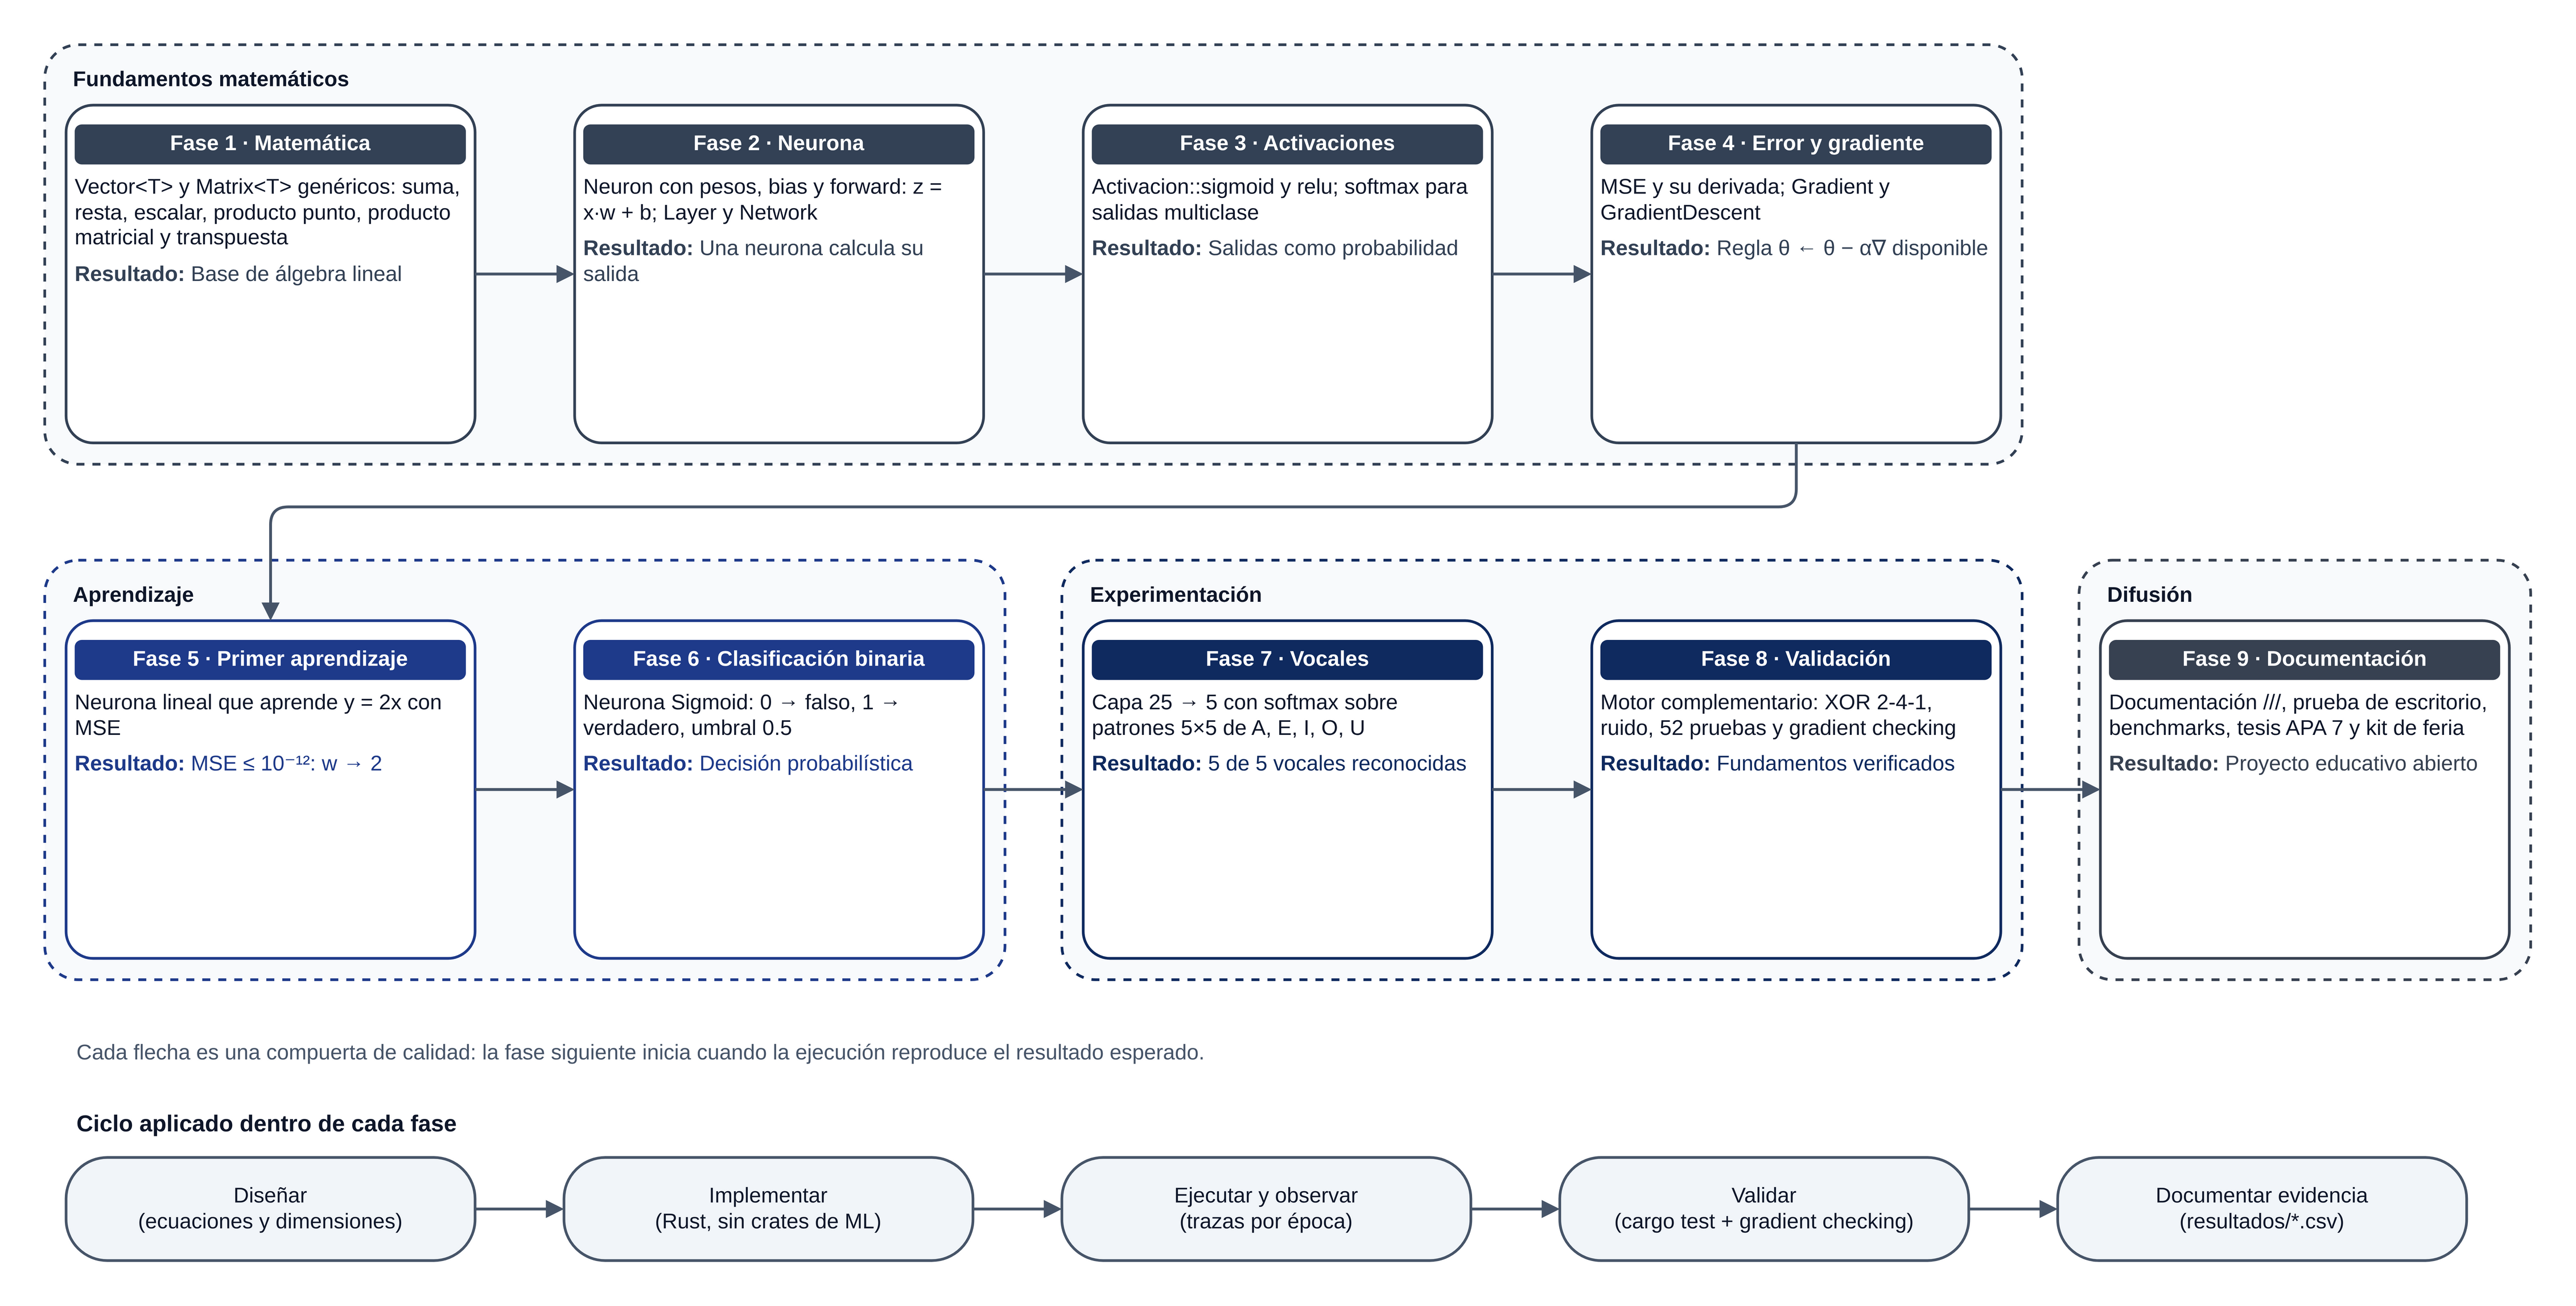
\includegraphics[width=\textwidth,height=0.5\textheight,keepaspectratio]{figuras/diag05_fases_metodologia.png}
\fuente{Cada fase concluye con la aprobación de sus pruebas unitarias. Diagrama editable: \texttt{diagramas/05\_fases\_metodologia.drawio}.}
\end{figure}

La Tabla~\ref{tab:fases} detalla las fases en forma tabular, junto con los módulos de código que producen y las pruebas que las validan.

\begin{table}[!htbp]
\caption{Fases de desarrollo, entregables y criterios de aceptación}\label{tab:fases}
\small
\begin{tabularx}{\textwidth}{@{}l >{\raggedright}p{3.4cm} >{\raggedright}X >{\raggedright\arraybackslash}p{3.6cm}@{}}
\toprule
Fase & Nombre & Entregable & Criterio de aceptación \\
\midrule
1 & Matemática & \texttt{Vector}, \texttt{Matrix}, \texttt{MathError}, \texttt{Rng} & 15 pruebas de \texttt{math} \\
2 & Neurona & \texttt{Neuron}: $z=\mathbf{w}\cdot\mathbf{x}+b$, $a=f(z)$ & Cálculo manual reproducido \\
3 & Activaciones & Sigmoid, ReLU y lineal con sus derivadas & Derivadas verificadas numéricamente \\
4 & Error & \texttt{Mse} y su gradiente $\partial L/\partial\hat{y}$ & Valores conocidos y \emph{gradient checking} \\
5 & Primer aprendizaje & Descenso de gradiente sobre $y=2x$ & El MSE disminuye y $w\to 2$ \\
6 & Capas y red & \texttt{Layer} y \texttt{Network}: \texttt{forward}, \texttt{backward}, \texttt{predict}, \texttt{train} & \emph{Gradient checking} de la red \\
7 & XOR & Perceptrón 2-1 frente a red 2-4-1 y tres tasas de aprendizaje & Aprendizaje no lineal demostrado \\
8 & Vocales & Red 25-10-5 sobre matrices $5\times5$ con ruido & Exactitud y matriz de confusión en CSV \\
9 & Documentación & Prueba de escritorio, \emph{benchmarks}, tesis, diagramas y material de feria & PDF y DOCX sin referencias rotas \\
\bottomrule
\end{tabularx}
\fuente{Elaboración propia. El número de pruebas por módulo se detalla en la Tabla~\ref{tab:pruebas}.}
\end{table}

\section{Requisitos del sistema}
Antes de diseñar la arquitectura se establecieron los requisitos funcionales y no funcionales que el motor debía cumplir. Los requisitos funcionales comprenden: representar vectores y matrices con sus operaciones; construir redes de topología arbitraria a partir de una lista de tamaños de capa y de funciones de activación; propagar una entrada hacia adelante; calcular el gradiente de la pérdida mediante retropropagación; actualizar los parámetros por descenso de gradiente; ejecutar los tres experimentos y la prueba de escritorio; medir tiempos; y exportar todos los resultados en formato CSV. Los requisitos no funcionales comprenden: no utilizar dependencias externas; garantizar la reproducibilidad exacta mediante una semilla; detectar los errores de dimensión sin interrumpir abruptamente el programa; documentar cada elemento público con comentarios \texttt{///}; y superar el análisis estático de \texttt{cargo clippy} sin advertencias.

\section{Arquitectura modular}
El código se organiza como una biblioteca (\texttt{src/lib.rs}) y un binario de línea de comandos (\texttt{src/main.rs}). La biblioteca se divide en tres módulos con responsabilidades separadas y dependencias en un solo sentido: \texttt{experiments} depende de \texttt{nn}, y \texttt{nn} depende de \texttt{math}, pero nunca a la inversa. La Figura~\ref{fig:arquitectura} representa esta organización.

\begin{figure}[!htbp]
\caption{Arquitectura modular del motor en Rust}\label{fig:arquitectura}
\centering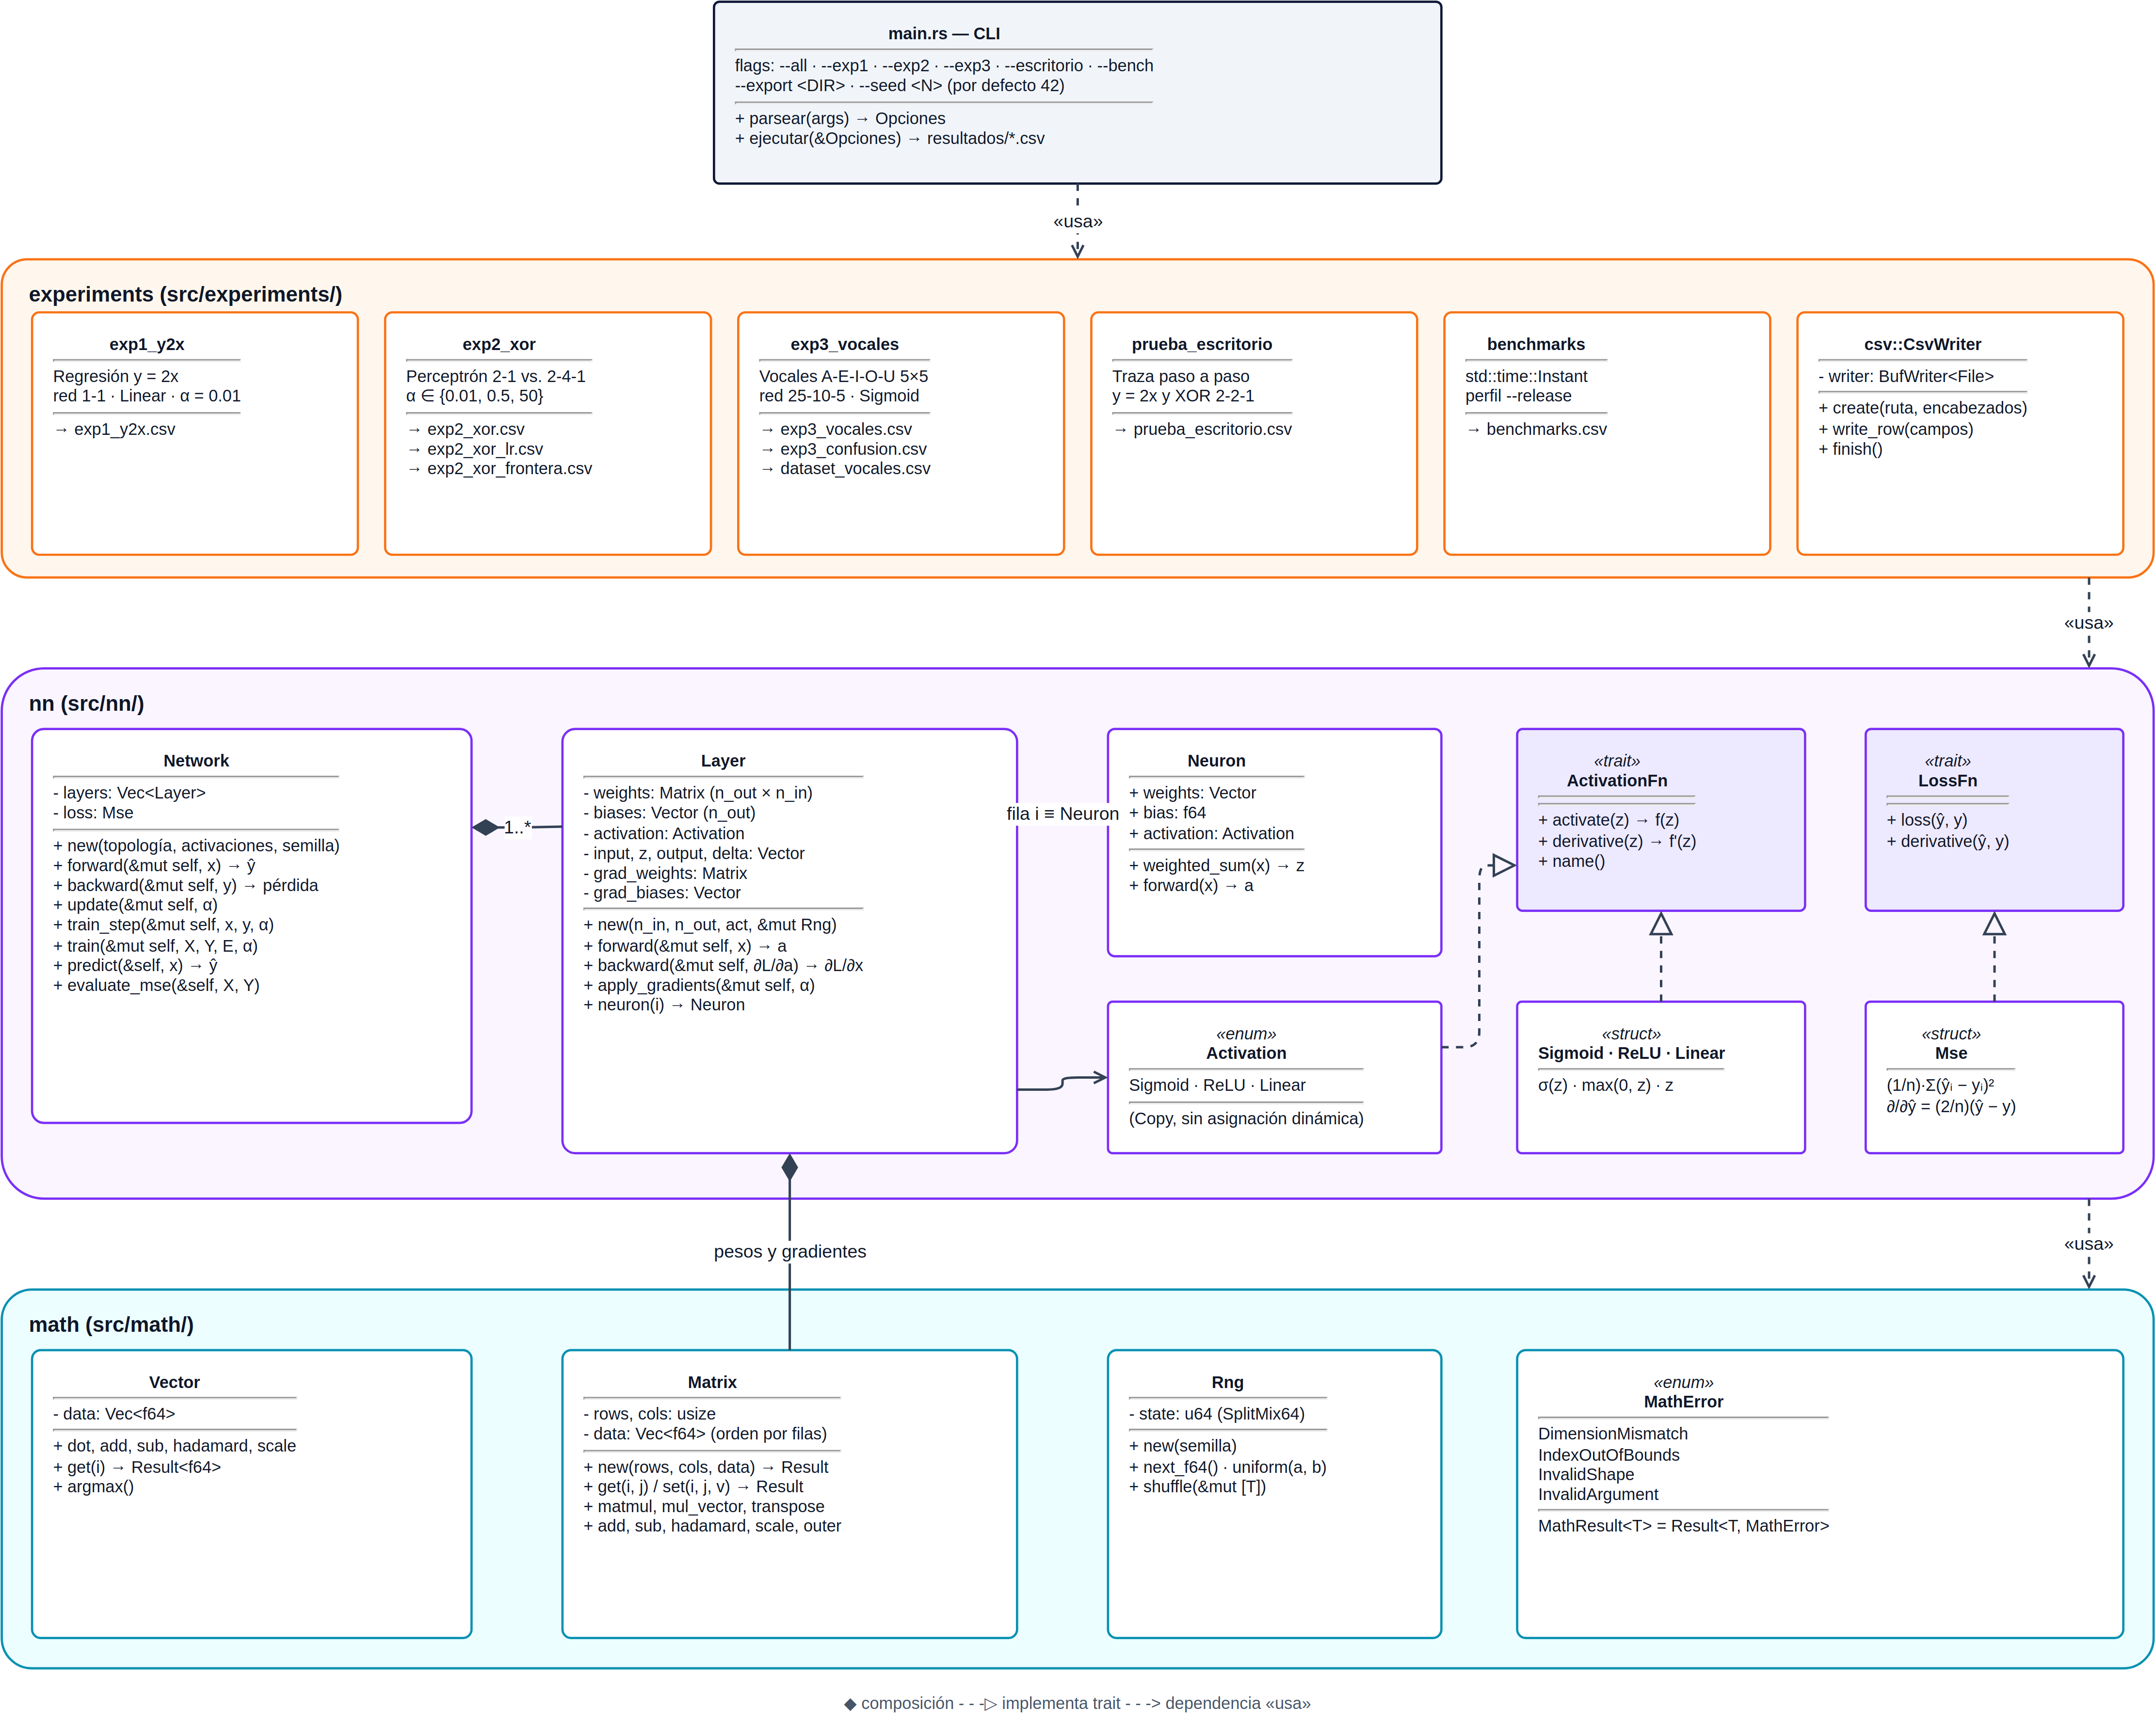
\includegraphics[width=\textwidth,height=0.55\textheight,keepaspectratio]{figuras/diag02_arquitectura_rust.png}
\fuente{Las flechas indican dependencias de uso entre módulos. Diagrama editable: \texttt{diagramas/02\_arquitectura\_modulos\_rust.drawio}.}
\end{figure}

La Tabla~\ref{tab:arquitectura} describe la responsabilidad de cada archivo. La separación permite probar cada componente de forma aislada y sustituirlo sin afectar a los demás; por ejemplo, la estructura \texttt{Network} no conoce la fórmula de ninguna función de activación, sino que delega en el trait \texttt{ActivationFn}.

\begin{table}[!htbp]
\caption{Módulos de la arquitectura implementada}\label{tab:arquitectura}
\small
\begin{tabularx}{\textwidth}{@{}l >{\raggedright\arraybackslash}X@{}}
\toprule
Archivo & Responsabilidad \\
\midrule
\texttt{math/vector.rs} & Vector $\mathbb{R}^n$: suma, resta, producto punto, Hadamard, escalamiento, norma, \texttt{argmax}. \\
\texttt{math/matrix.rs} & Matriz $\mathbb{R}^{m\times n}$ \emph{row-major}: producto matricial, matriz-vector, transpuesta, producto exterior. \\
\texttt{math/error.rs} & Tipo \texttt{MathError} para dimensiones incompatibles, índices fuera de rango y argumentos inválidos. \\
\texttt{math/rng.rs} & Generador pseudoaleatorio SplitMix64 reproducible y barajado Fisher--Yates. \\
\texttt{nn/activation.rs} & Trait \texttt{ActivationFn}; Sigmoid, ReLU y lineal con derivadas analíticas. \\
\texttt{nn/loss.rs} & Trait \texttt{LossFn}; MSE y su gradiente. \\
\texttt{nn/neuron.rs} & Neurona individual: pesos, sesgo, suma ponderada y activación. \\
\texttt{nn/layer.rs} & Capa densa: \texttt{forward}, \texttt{backward}, gradientes y actualización. \\
\texttt{nn/network.rs} & Red multicapa: \texttt{forward}, \texttt{backward}, \texttt{predict}, \texttt{train}, evaluación. \\
\texttt{experiments/} & Tres experimentos, prueba de escritorio, \emph{benchmarks} y escritura de CSV. \\
\texttt{main.rs} & CLI reproducible: \texttt{--all}, \texttt{--exp1..3}, \texttt{--escritorio}, \texttt{--bench}, \texttt{--export}, \texttt{--seed}. \\
\bottomrule
\end{tabularx}
\fuente{El archivo \texttt{Cargo.toml} no declara ninguna dependencia: todo el sistema utiliza exclusivamente la biblioteca estándar de Rust.}
\end{table}

\section{Decisiones de diseño}
Varias decisiones de diseño condicionan el comportamiento del sistema y merecen justificarse explícitamente.

\subsection{Almacenamiento contiguo por filas}
Se eligió almacenar cada matriz en un único \texttt{Vec<f64>} en lugar de un vector de vectores. Esta representación reduce el número de reservas de memoria, mejora la localidad de referencia en el producto matriz-vector ---que recorre cada fila de forma secuencial--- y simplifica la validación de dimensiones, pues basta comprobar que la longitud del arreglo sea $m\cdot n$.

\subsection{Errores como valores}
Todas las operaciones susceptibles de fallar devuelven \texttt{Result}. La alternativa ---provocar un pánico ante dimensiones incompatibles--- habría sido más breve, pero habría impedido probar los casos de error y habría convertido un descuido de configuración en una terminación abrupta del programa. Las pruebas \texttt{errores\_de\_dimension}, \texttt{mse\_errores\_de\_dimension} y \texttt{backward\_sin\_forward\_es\_error} verifican precisamente estos caminos.

\subsection{Caché de valores intermedios en la capa}
Cada capa guarda la última entrada recibida, el vector $\mathbf{z}$, la salida, el vector $\boldsymbol{\delta}$ y los gradientes. Esta decisión, que cuesta memoria proporcional al tamaño de la capa, evita recalcular la propagación hacia adelante durante la retropropagación y permite que la prueba de escritorio lea directamente los valores intermedios de cada neurona. Para la inferencia se ofrece además el método \texttt{predict}, que recibe la red por referencia inmutable y no modifica la caché.

\subsection{Generador pseudoaleatorio propio}
La biblioteca estándar de Rust no incluye un generador de números aleatorios con semilla. En lugar de añadir una dependencia, se implementó SplitMix64, un generador de 64 bits con buena calidad estadística para inicialización y muestreo, cuya secuencia de referencia se verifica en la prueba \texttt{vector\_de\_referencia\_splitmix64}. La semilla por defecto es 42 y puede modificarse con el argumento \texttt{--seed}.

\subsection{Activaciones mediante trait y enumeración}
Las funciones de activación implementan el trait \texttt{ActivationFn}, y la enumeración \texttt{Activation} despacha a cada implementación mediante \texttt{match}. Esta combinación permite guardar la activación de cada capa como un valor pequeño y copiable, compararla y exportarla por nombre, mientras que el trait conserva la posibilidad de extender el sistema con nuevas funciones.

\section{Flujo de entrenamiento}
La Figura~\ref{fig:flujo} representa el algoritmo de entrenamiento implementado. Una iteración consta de cuatro pasos: (1) la entrada $\mathbf{x}$ atraviesa cada capa calculando $\mathbf{z}^{(l)}$ y $\mathbf{a}^{(l)}$, que se almacenan en caché; (2) se calcula la pérdida MSE y su gradiente respecto a la salida; (3) cada capa, de la última a la primera, calcula $\boldsymbol{\delta}^{(l)}$, sus gradientes y el gradiente que transmite a la capa anterior; y (4) todos los parámetros se actualizan con la Ecuación~\eqref{eq:gd}. Al terminar cada época se evalúa el MSE sobre el conjunto completo y se registra en el archivo CSV del experimento.

\begin{figure}[!htbp]
\caption{Diagrama de flujo del entrenamiento con propagación hacia adelante y retropropagación}\label{fig:flujo}
\centering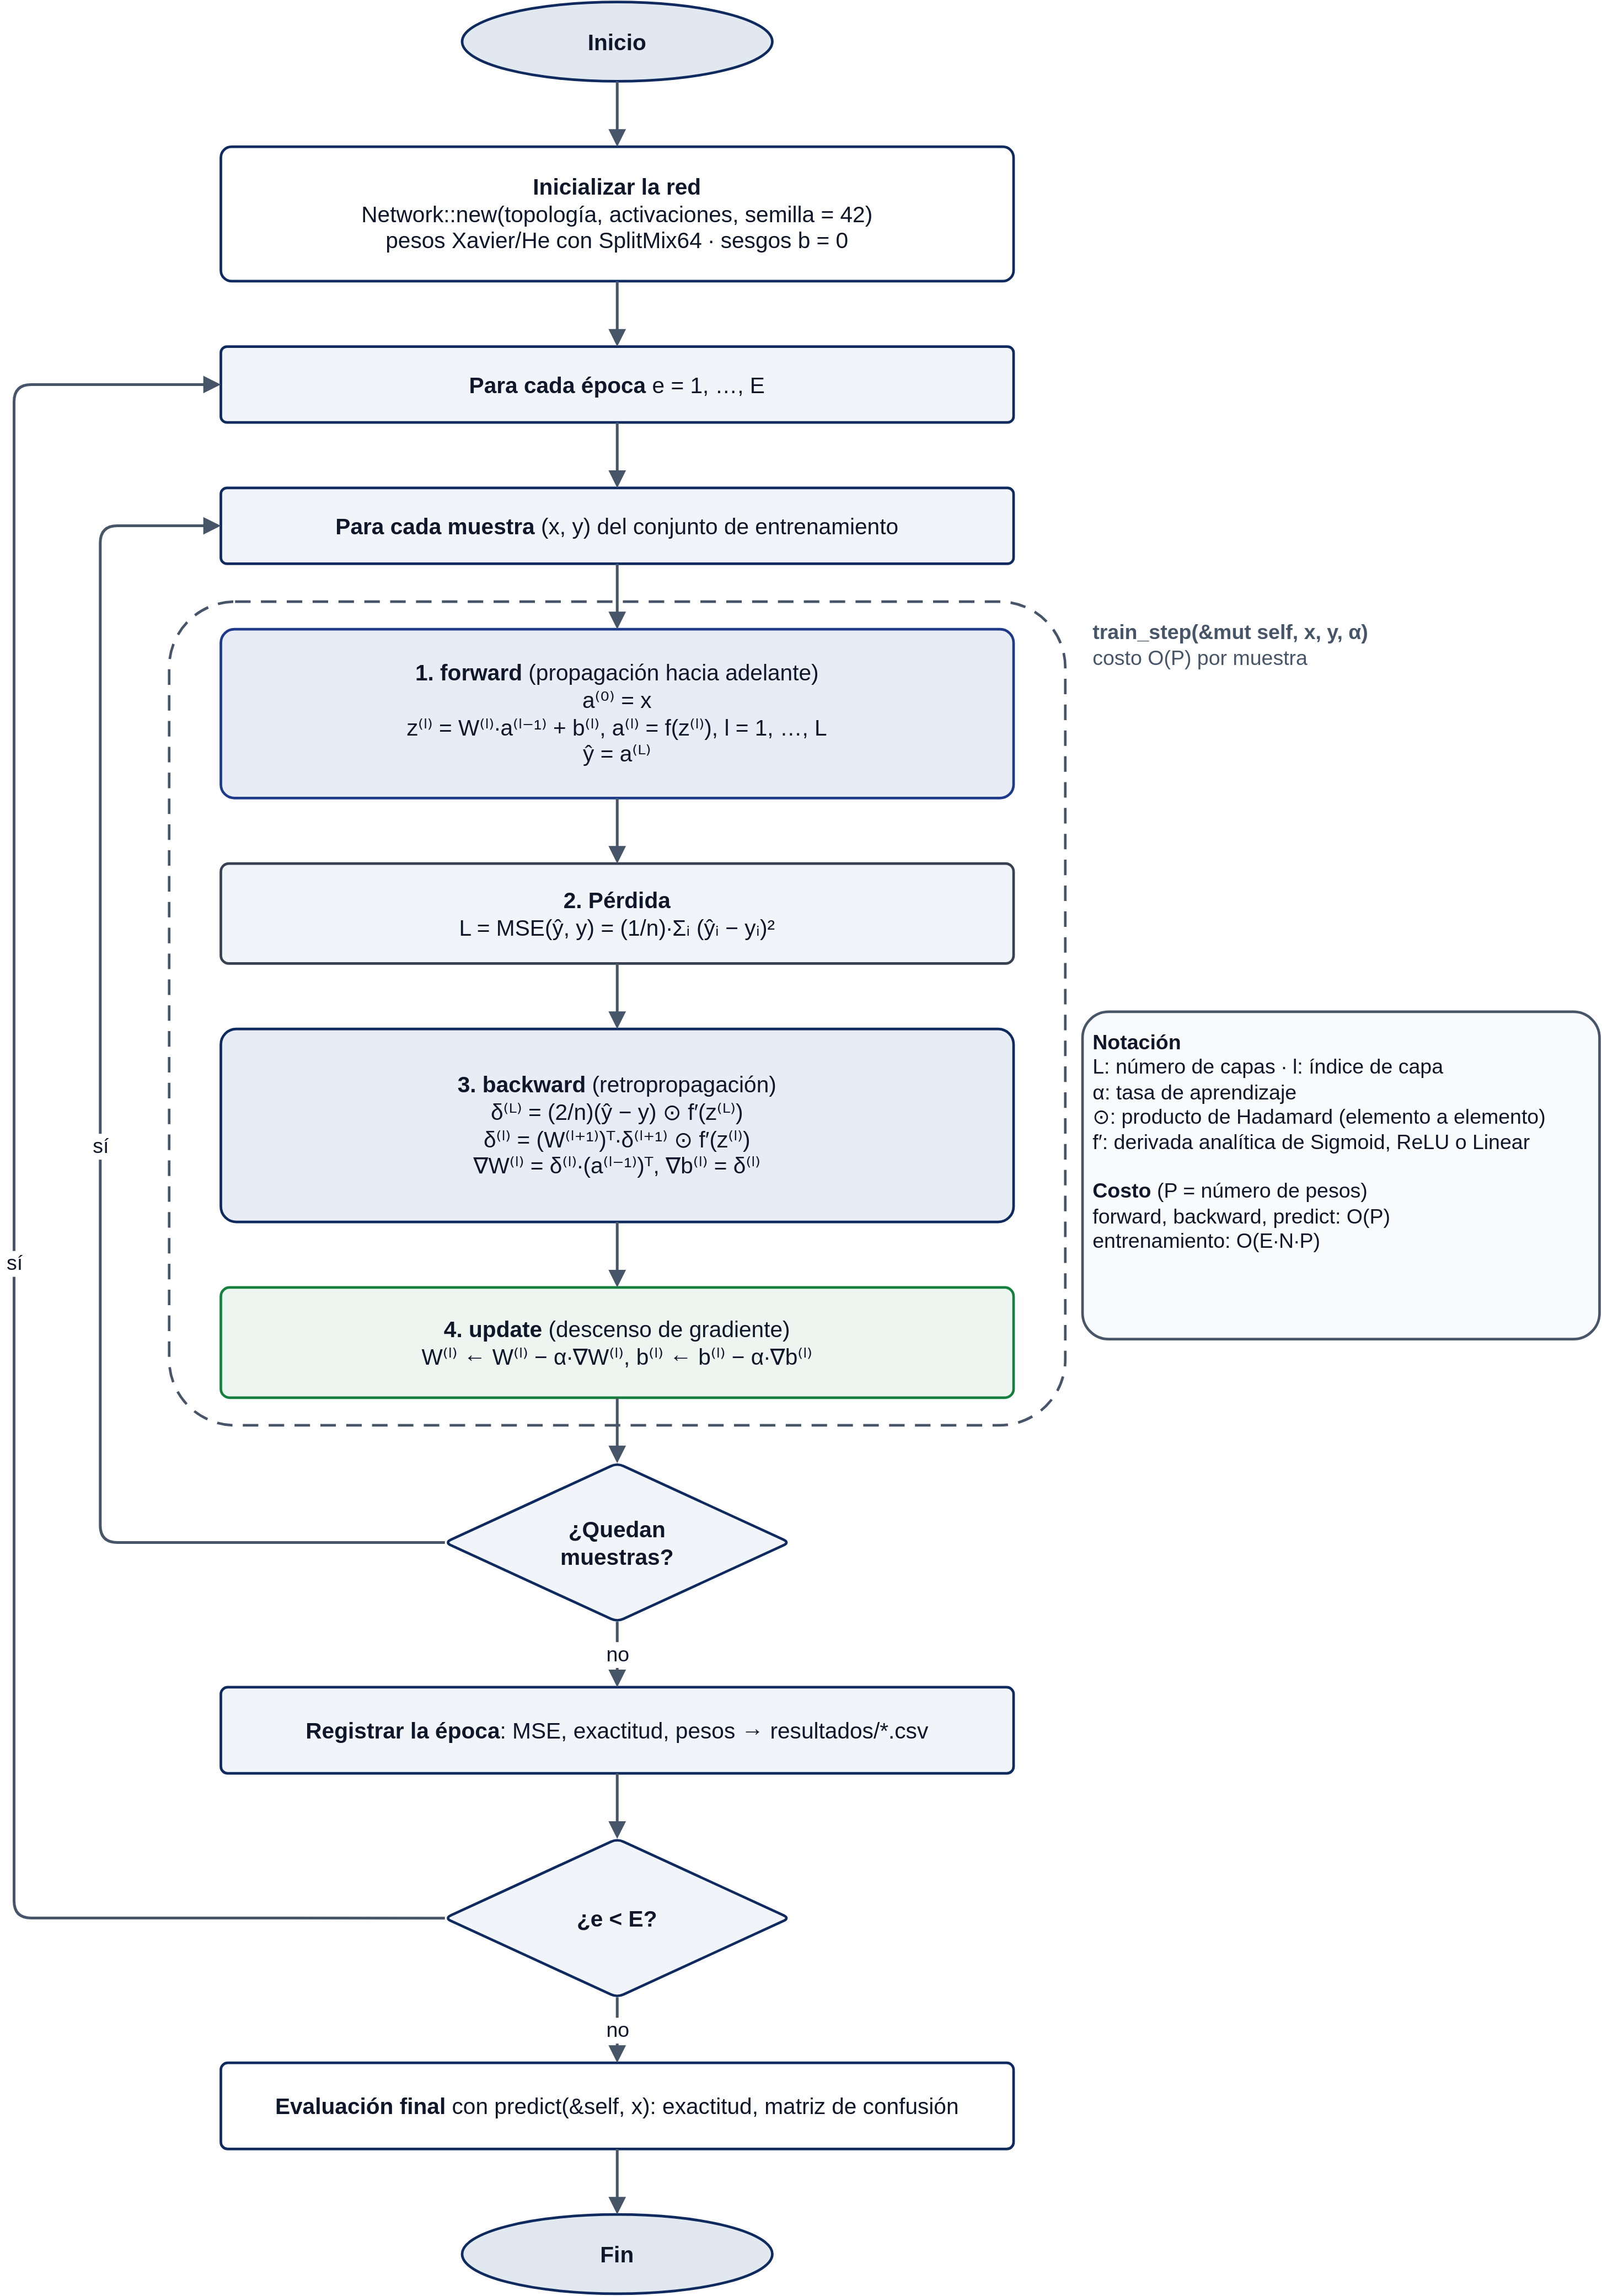
\includegraphics[width=\textwidth,height=0.72\textheight,keepaspectratio]{figuras/diag03_flujo_entrenamiento.png}
\fuente{El ciclo interno recorre las muestras y el externo las épocas. Diagrama editable: \texttt{diagramas/03\_flujo\_forward\_backprop.drawio}.}
\end{figure}

\section{Estrategia de verificación}
La verificación combina cuatro tipos de pruebas automatizadas. Las pruebas de valores conocidos comparan la salida de una función con un resultado calculado a mano, por ejemplo $\sigma(0) = 0.5$ o la salida de una capa con pesos fijos. Las pruebas de errores comprueban que las operaciones con dimensiones incompatibles devuelvan el error esperado. Las pruebas de propiedades verifican identidades matemáticas y de determinismo, como que la misma semilla produzca la misma secuencia o que el barajado sea una permutación. Finalmente, las pruebas de integración entrenan redes reales y verifican su convergencia y la corrección numérica de sus gradientes. La Tabla~\ref{tab:pruebas} presenta la distribución de las 52 pruebas por módulo.

\begin{table}[!htbp]
\caption{Distribución de las pruebas automatizadas por módulo}\label{tab:pruebas}
\small
\begin{tabularx}{\textwidth}{@{}l r >{\raggedright\arraybackslash}X@{}}
\toprule
Módulo & Pruebas & Aspectos verificados \\
\midrule
\texttt{math::vector} & 4 & Creación, acceso seguro, operaciones, \texttt{argmax}, errores de dimensión \\
\texttt{math::matrix} & 6 & Acceso, operaciones elemento a elemento, producto matricial, transpuesta, producto exterior \\
\texttt{math::rng} & 4 & Secuencia de referencia, determinismo, rangos uniformes, permutación \\
\texttt{math::error} & 1 & Mensajes descriptivos \\
\texttt{nn::activation} & 4 & Valores conocidos, despacho, derivadas por \emph{gradient checking} \\
\texttt{nn::loss} & 3 & Valores conocidos, errores, \emph{gradient checking} \\
\texttt{nn::neuron} & 3 & Cálculo manual, errores, inicialización reproducible \\
\texttt{nn::layer} & 4 & Dimensiones, cálculo manual, retropropagación y actualización \\
\texttt{nn::network} & 11 & Validaciones, \emph{gradient checking} (2-4-1, 3-5-4-2, 25-10-5), convergencia \\
\texttt{experiments} & 11 & CSV, exactitud, experimentos 1--3, prueba de escritorio, \emph{benchmarks} \\
\texttt{main} (CLI) & 1 & Interpretación de argumentos y errores \\
\midrule
Total & 52 & 51 pruebas de biblioteca y 1 de binario \\
\bottomrule
\end{tabularx}
\fuente{Conteo obtenido de la salida real de \texttt{cargo test} (Anexo~\ref{anx:tests}).}
\end{table}

\section{Reproducibilidad}
Para que cualquier evaluador obtenga exactamente los mismos resultados, se tomaron tres medidas. Primero, todos los pesos iniciales, el orden aleatorio y el ruido de los datos se generan con el PRNG propio a partir de una semilla fija, de modo que la misma semilla produce los mismos números en cualquier equipo. Segundo, los conjuntos de datos se definen explícitamente en el código fuente y no dependen de archivos externos. Tercero, el binario escribe todos los resultados en archivos CSV, y las tablas, cifras y gráficas de este documento se generan exclusivamente a partir de esos archivos mediante los scripts \path{tesis/scripts/resultados.py} y \path{scripts/generar_graficas.py}. La presentación de tablas, figuras, citas y referencias sigue el manual de publicaciones de la American Psychological Association en su séptima edición \citep{apa2020}. Los tiempos de ejecución son la única magnitud que depende del equipo; por ello se informan junto con el sistema operativo, la arquitectura y el perfil de compilación.

\section{Diseño de los experimentos}
Los tres experimentos se diseñaron con complejidad creciente, de modo que cada uno valide una capacidad adicional del motor. La Tabla~\ref{tab:diseno-exp} resume su configuración.

\begin{table}[!htbp]
\caption{Configuración de los experimentos}\label{tab:diseno-exp}
\footnotesize
\begin{tabularx}{\textwidth}{@{}l >{\raggedright}X >{\raggedright}X >{\raggedright\arraybackslash}X@{}}
\toprule
Aspecto & Experimento 1 & Experimento 2 & Experimento 3 \\
\midrule
Problema & Regresión $y=2x$ & Compuerta XOR & Vocales A, E, I, O, U \\
Capacidad validada & Ajuste lineal & Separación no lineal & Clasificación multiclase con ruido \\
Arquitectura & 1-1 (lineal) & 2-1 y 2-4-1 (Sigmoid) & 25-10-5 (Sigmoid) \\
Parámetros & 2 & 3 y 17 & 315 \\
Épocas & \EunoEpocas & \EdosEpocas & \EtresEpocas \\
Tasa $\alpha$ & \EunoAlpha & \EdosAlpha{} (y 0.01, 50) & \EtresAlpha \\
Datos & 5 pares $(x, 2x)$ & 4 combinaciones binarias & \EtresNEnt{} de entrenamiento, \EtresNPru{} de prueba \\
Métricas & MSE, $w$, $b$, predicción & MSE, exactitud, frontera & MSE, exactitud, confusión \\
\bottomrule
\end{tabularx}
\fuente{Valores leídos de \path{resultados/resumen.csv}. Todas las ejecuciones usan semilla 42.}
\end{table}

El Experimento~1 tiene solución analítica conocida ($w=2$, $b=0$), por lo que permite verificar cuantitativamente la convergencia. El Experimento~2 reproduce el argumento histórico de \citet{minsky1969} y su superación mediante una capa oculta, y añade un estudio del efecto de la tasa de aprendizaje. El Experimento~3 introduce un problema multiclase con 25 entradas, separa estrictamente los conjuntos de entrenamiento y de prueba y evalúa la robustez frente a niveles de ruido mayores que los vistos durante el entrenamiento.

\chapter{Implementación, Experimentos y Resultados}\label{cap:implementacion}
Este capítulo presenta, en primer lugar, la implementación y los resultados del repositorio oficial del equipo, \url{\Repositorio} (commit \texttt{\OfCommit}), que es el sistema que se demuestra en la feria. En segundo lugar, resume la validación complementaria realizada con el motor extendido \url{\RepositorioMotor}. Las cifras del repositorio oficial provienen de \path{resultados/oficial/*.csv}, generados por \path{scripts/auditar_repo_oficial.py} a partir de la salida real del binario; las del motor complementario provienen de \path{resultados/*.csv}, generados con \texttt{cargo run --release -- --all} y semilla 42. Ninguna tabla ni gráfica se ha editado manualmente.

\section{Implementación del repositorio oficial}
La implementación traduce las ecuaciones del Capítulo~\ref{cap:marco} en funciones breves sobre números \texttt{f32}. Esta sección recorre los componentes en el orden en que intervienen durante el entrenamiento.

\subsection{Neurona, capa y red}
La neurona (Código~\ref{cod:of-neuron}) calcula la suma ponderada de la Ecuación~\eqref{eq:neurona} mediante el producto punto de \texttt{Vector} y comprueba con \texttt{assert\_eq!} que las dimensiones coincidan. La capa (Código~\ref{cod:of-layer}) aplica cada neurona a la misma entrada y reúne las salidas en un nuevo vector; la red (Código~\ref{cod:of-network}) encadena las capas. La activación no forma parte de la neurona: cada experimento la aplica sobre la salida lineal $z$.

\lstinputlisting[caption={Propagación de una neurona (\texttt{src/neural/neuron.rs})},label=cod:of-neuron]{generado/codigo/of_neuron.rs}
\needspace{8\baselineskip}\lstinputlisting[caption={Propagación de una capa (\texttt{src/neural/layer.rs})},label=cod:of-layer]{generado/codigo/of_layer.rs}
\lstinputlisting[caption={Propagación de la red (\texttt{src/neural/network.rs})},label=cod:of-network]{generado/codigo/of_network.rs}

\subsection{Activaciones, pérdida, gradiente y optimizador}
El Código~\ref{cod:of-activacion} implementa Sigmoid y ReLU según las Ecuaciones~\eqref{eq:sigmoid} y~\eqref{eq:relu}. El Código~\ref{cod:of-mse} implementa el MSE y su derivada (Ecuación~\eqref{eq:mse}); el Código~\ref{cod:of-gradient} convierte el error de una salida en los gradientes de sus pesos y de su bias, y el Código~\ref{cod:of-optimizer} aplica la regla de descenso de gradiente de la Ecuación~\eqref{eq:gd}.

\lstinputlisting[caption={Funciones de activación (\texttt{src/neural/activation.rs})},label=cod:of-activacion]{generado/codigo/of_activacion.rs}
\lstinputlisting[caption={Error cuadrático medio y su derivada (\texttt{src/learning/loss.rs})},label=cod:of-mse]{generado/codigo/of_mse.rs}
\needspace{8\baselineskip}\lstinputlisting[caption={Gradientes de pesos y bias (\texttt{src/learning/gradient.rs})},label=cod:of-gradient]{generado/codigo/of_gradient.rs}
\lstinputlisting[caption={Descenso de gradiente (\texttt{src/learning/optimizer.rs})},label=cod:of-optimizer]{generado/codigo/of_optimizer.rs}

\subsection{Softmax y decisión multiclase}
El experimento de vocales convierte las cinco salidas lineales en probabilidades con la función softmax de la Ecuación~\eqref{eq:softmax} (Código~\ref{cod:of-softmax}). Antes de exponenciar se resta el máximo, lo que no altera el resultado pero evita desbordamientos. La clase reconocida es la de mayor probabilidad (Código~\ref{cod:of-argmax}).

\lstinputlisting[caption={Softmax numéricamente estable (\texttt{src/experiments/vowels.rs})},label=cod:of-softmax]{generado/codigo/of_softmax.rs}
\lstinputlisting[caption={Índice de la probabilidad máxima (\texttt{src/experiments/vowels.rs})},label=cod:of-argmax]{generado/codigo/of_argmax.rs}

\section{Experimento oficial 1: aprender $y=2x$}\label{sec:of-lineal}
Una neurona lineal con peso y bias iniciales en cero aprende la relación $y=2x$ a partir de \OfLinN{} muestras ($x\in\{1,2,3,4,7,8\}$), con $\alpha=\OfLinAlpha$ y pérdida MSE. En cada época se acumula el gradiente de todas las muestras y se actualizan los parámetros una sola vez (descenso de gradiente por lote completo, Código~\ref{cod:of-lin}); el entrenamiento se detiene cuando el MSE es menor o igual que $10^{-12}$ o al llegar a 10\,000 épocas.

\lstinputlisting[caption={Época de entrenamiento de la regresión $y=2x$ (\texttt{src/experiments/linear.rs})},label=cod:of-lin]{generado/codigo/of_lin_epoca.rs}

La meta se alcanzó en la época \OfLinEpocas{}: el MSE descendió de \OfLinMseIni{} a \OfLinMseFin, con $w=\OfLinPeso$ y $b=\OfLinBias$. La Tabla~\ref{tab:of-lineal} muestra la evolución registrada por el programa, que informa cada 20 épocas, y la Figura~\ref{fig:of-lineal} la representa gráficamente.

\begin{table}[!htbp]
\caption{Evolución del entrenamiento oficial de $y=2x$}\label{tab:of-lineal}
\small
\begin{tabular*}{\textwidth}{@{\extracolsep{\fill}}rrrr@{}}
\toprule
Época & Peso $w$ & Bias $b$ & MSE \\
\midrule
\TablaOfLineal
\bottomrule
\end{tabular*}
\fuente{Fuente: \path{resultados/oficial/lineal.csv}, extraído de la salida de \texttt{cargo run -- lineal}.}
\end{table}

\begin{figure}[!htbp]
\caption{Pérdida y parámetros del experimento oficial $y=2x$}\label{fig:of-lineal}
\centering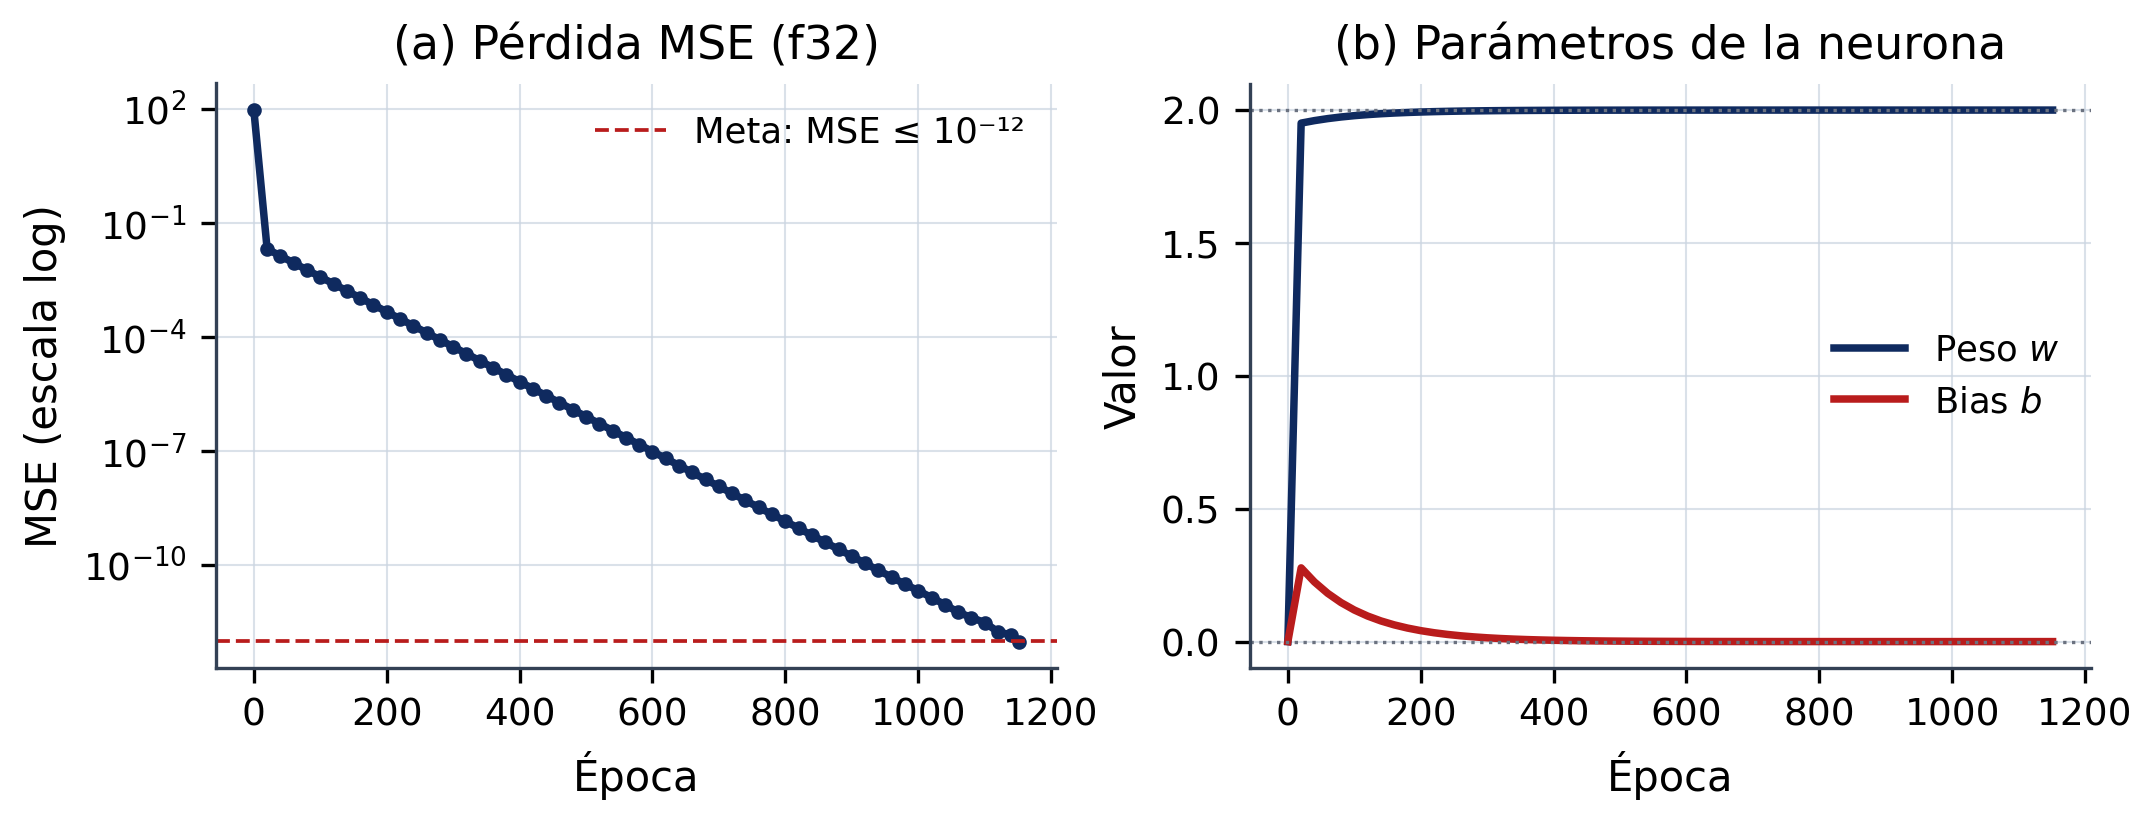
\includegraphics[width=\textwidth]{figuras/fig12_oficial_lineal.png}
\fuente{(a) MSE en escala logarítmica con la meta de $10^{-12}$. (b) Peso y bias. Fuente: \path{resultados/oficial/lineal.csv}.}
\end{figure}

\begin{table}[!htbp]
\caption{Predicciones finales del experimento oficial $y=2x$}\label{tab:of-linpred}
\small
\begin{tabular*}{0.7\textwidth}{@{\extracolsep{\fill}}rrrr@{}}
\toprule
$x$ & Esperado & Predicción & Error \\
\midrule
\TablaOfLinPred
\bottomrule
\end{tabular*}
\fuente{Error $=\hat{y}-y$, con la precisión que imprime el programa. Fuente: \path{resultados/oficial/lineal_predicciones.csv}.}
\end{table}

La pérdida decrece de forma aproximadamente exponencial, como corresponde a un problema cuadrático convexo con una tasa de aprendizaje estable. El salto inicial de 95.33 a 0.02 en las primeras 20 épocas refleja que el peso se acerca a 2 casi de inmediato, mientras el bias, que crece al principio para compensar el error, tarda cientos de épocas en volver a cero. Los errores residuales del orden de $10^{-6}$ de la Tabla~\ref{tab:of-linpred} son el límite práctico de la aritmética \texttt{f32}.

\section{Experimento oficial 2: clasificación booleana}\label{sec:of-bool}
Una neurona Sigmoid aprende a clasificar la entrada 0 como falso y la entrada 1 como verdadero; la clase se decide con el umbral $0.5$. El gradiente de cada muestra es $(p-y)/N$ (Código~\ref{cod:of-bool}), que coincide con la Ecuación~\eqref{eq:ce} para la entropía cruzada binaria. Se entrena durante \OfBoolEpocas{} épocas con $\alpha=\OfBoolAlpha$ y el programa imprime en cada época los gradientes y la actualización de los parámetros.

\lstinputlisting[caption={Gradiente de la clasificación booleana (\texttt{src/experiments/true\_false.rs})},label=cod:of-bool]{generado/codigo/of_bool_muestras.rs}

Al final, $w=\OfBoolW$ y $b=\OfBoolB$; la probabilidad de verdadero es \OfBoolPcero{} para la entrada 0 y \OfBoolPuno{} para la entrada 1, de modo que ambas se clasifican correctamente (exactitud \OfBoolAcc). La Tabla~\ref{tab:of-bool} y la Figura~\ref{fig:of-bool} muestran la evolución.

\begin{table}[!htbp]
\caption{Traza del experimento oficial de clasificación booleana}\label{tab:of-bool}
\footnotesize
\begin{tabular*}{\textwidth}{@{\extracolsep{\fill}}rrrrrrr@{}}
\toprule
Época & $\nabla w$ & $\nabla b$ & $w$ & $b$ & $\sigma(b)$ & $\sigma(w+b)$ \\
\midrule
\TablaOfBool
\bottomrule
\end{tabular*}
\fuente{$\sigma(b)$ y $\sigma(w+b)$ son la probabilidad de verdadero para las entradas 0 y 1, calculadas con los parámetros impresos al final de cada época. Fuente: \path{resultados/oficial/booleano.csv}.}
\end{table}

\begin{figure}[!htbp]
\caption{Parámetros y probabilidades del experimento oficial booleano}\label{fig:of-bool}
\centering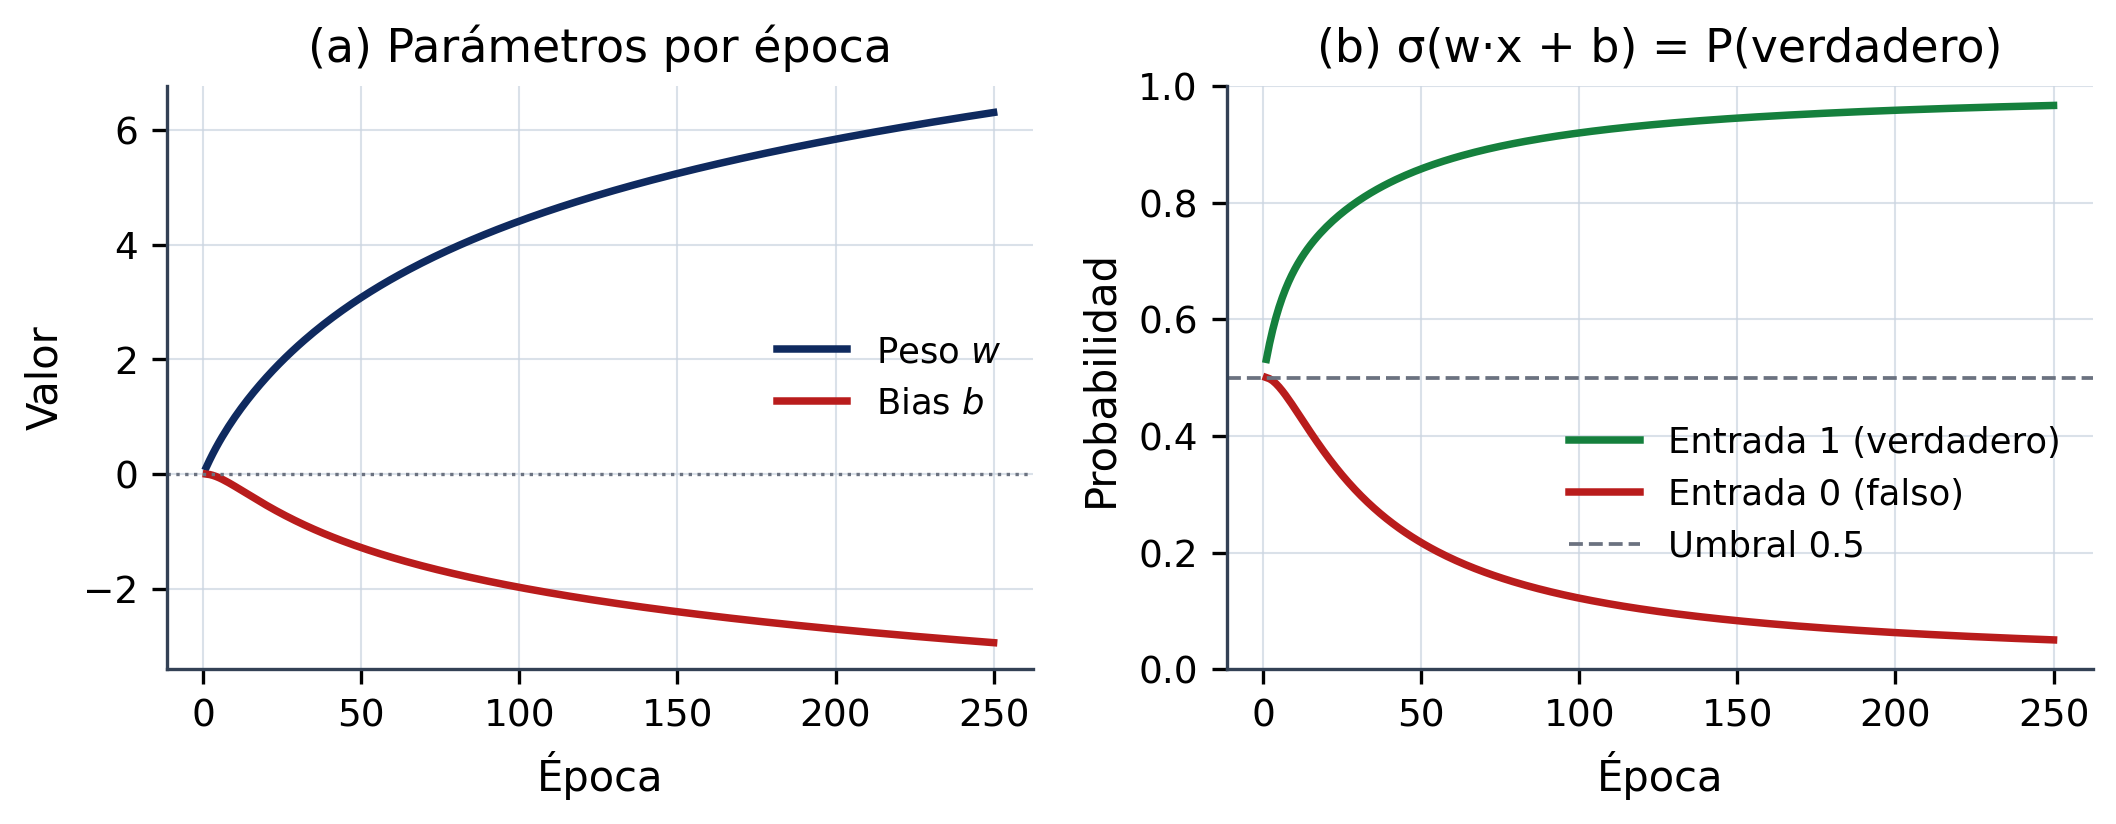
\includegraphics[width=\textwidth]{figuras/fig13_oficial_booleano.png}
\fuente{Fuente: \path{resultados/oficial/booleano.csv}.}
\end{figure}

En la primera época el bias no cambia: con parámetros nulos ambas probabilidades valen $0.5$ y los errores $(0.5-0)$ y $(0.5-1)$ se cancelan. A partir de allí el peso crece y el bias se vuelve negativo, separando las dos probabilidades del umbral. Como el problema es linealmente separable, una sola neurona basta; el problema XOR, que no lo es, se analiza con el motor complementario en la Sección~\ref{sec:exp2}.

\section{Experimento oficial 3: reconocimiento de vocales}\label{sec:of-voc}
Cada vocal se dibuja como una cuadrícula binaria de $5\times5$ (Figura~\ref{fig:of-voc}a) y se aplana en 25 entradas. Una capa de cinco neuronas, una por vocal, produce cinco puntuaciones que softmax convierte en probabilidades; la salida esperada es un vector \emph{one-hot}. El entrenamiento usa \OfVocEpocas{} épocas, $\alpha=\OfVocAlpha$ y descenso de gradiente por lote completo: el Código~\ref{cod:of-voc} acumula los gradientes de las cinco muestras y el Código~\ref{cod:of-vocupd} actualiza las neuronas.

\lstinputlisting[caption={Acumulación de gradientes con softmax (\texttt{src/experiments/vowels.rs})},label=cod:of-voc]{generado/codigo/of_voc_muestras.rs}
\lstinputlisting[caption={Actualización de las cinco neuronas (\texttt{src/experiments/vowels.rs})},label=cod:of-vocupd]{generado/codigo/of_voc_update.rs}

La red reconoce las cinco vocales con una confianza final entre \OfVocConfMin{} y \OfVocConfMax, y la orden \texttt{cargo run -- vocal a} reconoce la A con \OfVocalAProb. La Tabla~\ref{tab:of-voc} y la Figura~\ref{fig:of-voc} muestran la evolución de la probabilidad asignada a la clase correcta.

\begin{table}[!htbp]
\caption{Probabilidad de la clase correcta por época en el experimento oficial de vocales}\label{tab:of-voc}
\footnotesize
\begin{tabular*}{\textwidth}{@{\extracolsep{\fill}}lrrrrrlrr@{}}
\toprule
Vocal & Ép. 1 & Ép. 10 & Ép. 50 & Ép. 100 & Ép. 500 & Reconocida & Confianza (\%) & \texttt{vocal a} (\%) \\
\midrule
\TablaOfVoc
\bottomrule
\end{tabular*}
\fuente{Probabilidades con dos decimales, como las imprime el programa. La última columna es la probabilidad asignada a cada vocal al evaluar el patrón A. Fuente: \path{resultados/oficial/vocales.csv} y \path{resultados/oficial/vocal_a.csv}.}
\end{table}

\begin{figure}[!htbp]
\caption{Patrones, probabilidades y convergencia del experimento oficial de vocales}\label{fig:of-voc}
\centering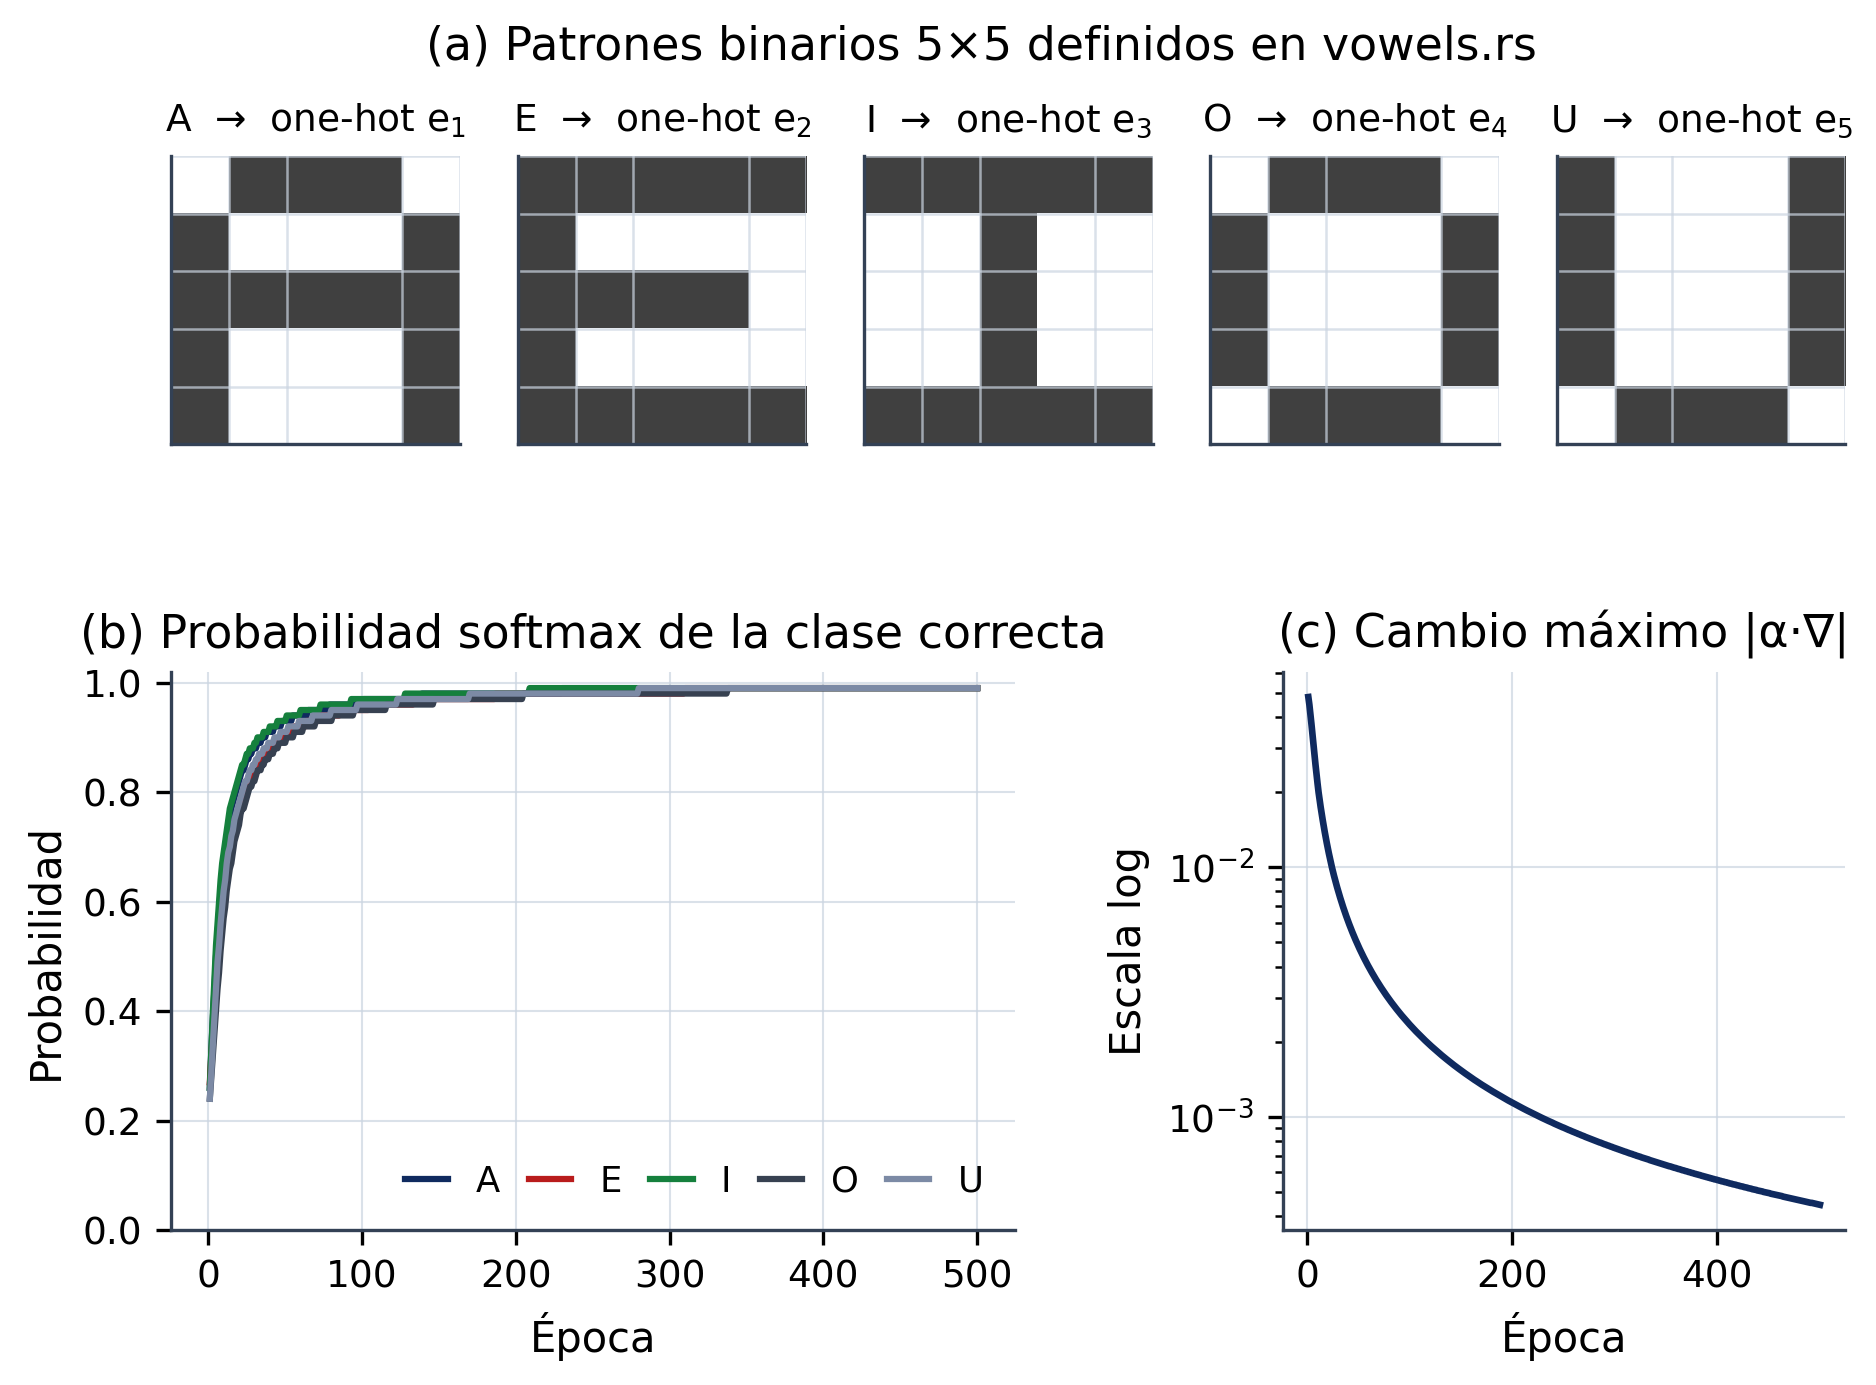
\includegraphics[width=\textwidth]{figuras/fig14_oficial_vocales.png}
\fuente{(c) Mayor cambio absoluto aplicado a un peso o bias en cada época. Fuente: \path{resultados/oficial/vocales.csv}.}
\end{figure}

Desde la primera época la probabilidad más alta corresponde a la vocal correcta, porque cada patrón activa sobre todo los pesos de su propia salida. El resto del entrenamiento aumenta la confianza y el cambio máximo por época desciende hasta \OfVocCambioFin, señal de convergencia. Como el conjunto contiene un único patrón por vocal y se evalúa con los mismos patrones, el resultado demuestra el mecanismo de aprendizaje pero no mide generalización; esa medición se realiza con el motor complementario (Sección~\ref{sec:exp3}).

\section{Tiempos de ejecución del repositorio oficial}\label{sec:of-tiempos}
El programa oficial incluye pausas \texttt{thread::sleep} para que la demostración pueda seguirse en pantalla. Por ello, la Tabla~\ref{tab:of-tiempos} informa dos tiempos: el de pared del binario oficial y el de cómputo de una copia idéntica a la que solo se le quitaron esas pausas (mediana de 5 ejecuciones, incluida la impresión en terminal). El binario \emph{release} ocupa \OfBinKiB~KiB.

\begin{table}[!htbp]
\caption{Tiempos de ejecución del repositorio oficial}\label{tab:of-tiempos}
\small
\begin{tabular*}{\textwidth}{@{\extracolsep{\fill}}llrr@{}}
\toprule
Experimento & Orden & Pared (s) & Cómputo sin pausas (ms) \\
\midrule
\TablaOfTiempos
\bottomrule
\end{tabular*}
\fuente{Linux x86\_64, rustc \OfRustc, perfil \emph{release}. Fuente: \path{resultados/oficial/resumen.csv}.}
\end{table}

\section{Validación complementaria con el motor extendido}\label{sec:complementario}
El repositorio oficial no define pruebas automatizadas ni entrena redes con capas ocultas. El motor extendido, escrito por el equipo en la etapa previa con la misma base matemática, cubre esos aspectos: implementa la retropropagación multicapa (Ecuaciones~\eqref{eq:deltaL}--\eqref{eq:gradW}) en \texttt{f64}, valida los gradientes con 52 pruebas automatizadas, resuelve XOR, evalúa las vocales con ruido y mide tiempos de entrenamiento e inferencia. Sus resultados no sustituyen a los del repositorio oficial: verifican de forma independiente las ecuaciones que este utiliza y muestran hasta dónde puede extenderse.

\subsection{Resultados de verificación}
La suite de pruebas cuenta con 52 pruebas automatizadas (51 en la biblioteca y 1 en la CLI), todas aprobadas. Incluyen valores calculados a mano, errores de dimensión, propiedades matemáticas, determinismo del PRNG, convergencia real de $y=2x$ y XOR, y verificación numérica de gradientes según la Ecuación~\eqref{eq:gradcheck} sobre redes 2-4-1, 3-5-4-2 y 25-10-5. Adicionalmente, \texttt{cargo clippy --all-targets} no reporta advertencias. La salida completa de ambas herramientas se reproduce en el Anexo~\ref{anx:tests}.

\subsection{Prueba de escritorio}\label{sec:escritorio}
La prueba de escritorio registra cada operación de las primeras iteraciones del entrenamiento y permite verificar con calculadora que el código ejecuta exactamente las fórmulas del marco teórico. Para la neurona lineal de $y=2x$ ($\alpha = 0.01$), la primera iteración con $x=1$, $y=2$ y parámetros iniciales $w_0 = \EunoPesoIni$, $b_0 = 0$ es:
\begin{align*}
z &= w_0 x + b_0 = 0.836805\cdot 1 + 0 = 0.836805, & a &= z = 0.836805,\\
e &= a - y = -1.163195, & \mathcal{L} &= e^2 = 1.353022,\\
\delta &= 2e\cdot f'(z) = -2.326389, & \partial\mathcal{L}/\partial w &= \delta\, x = -2.326389,\\
w_1 &= w_0 - \alpha\,\delta x = 0.860069, & b_1 &= b_0 - \alpha\,\delta = 0.023264.
\end{align*}
La Tabla~\ref{tab:escritorio} resume las diez primeras iteraciones (dos épocas) y la Figura~\ref{fig:escritorio} muestra la evolución de los parámetros a lo largo de esas iteraciones.

\begin{table}[!htbp]
\caption{Prueba de escritorio de la neurona lineal para $y=2x$ (primeras 10 iteraciones)}\label{tab:escritorio}
\footnotesize\setlength{\tabcolsep}{3.5pt}
\begin{tabular*}{\textwidth}{@{\extracolsep{\fill}}rrrrrrrrrr@{}}
\toprule
It. & $x$ & $y$ & $w$ & $b$ & $z$ & $e$ & $\partial\mathcal{L}/\partial w$ & $w'$ & $b'$ \\
\midrule
\TablaEscritorio
\bottomrule
\end{tabular*}
\fuente{$e = \hat{y}-y$; $w'$ y $b'$ son los parámetros después de la actualización. Fuente: \path{resultados/prueba_escritorio.csv}.}
\end{table}

\begin{figure}[!htbp]
\caption{Evolución de los parámetros durante la prueba de escritorio}\label{fig:escritorio}
\centering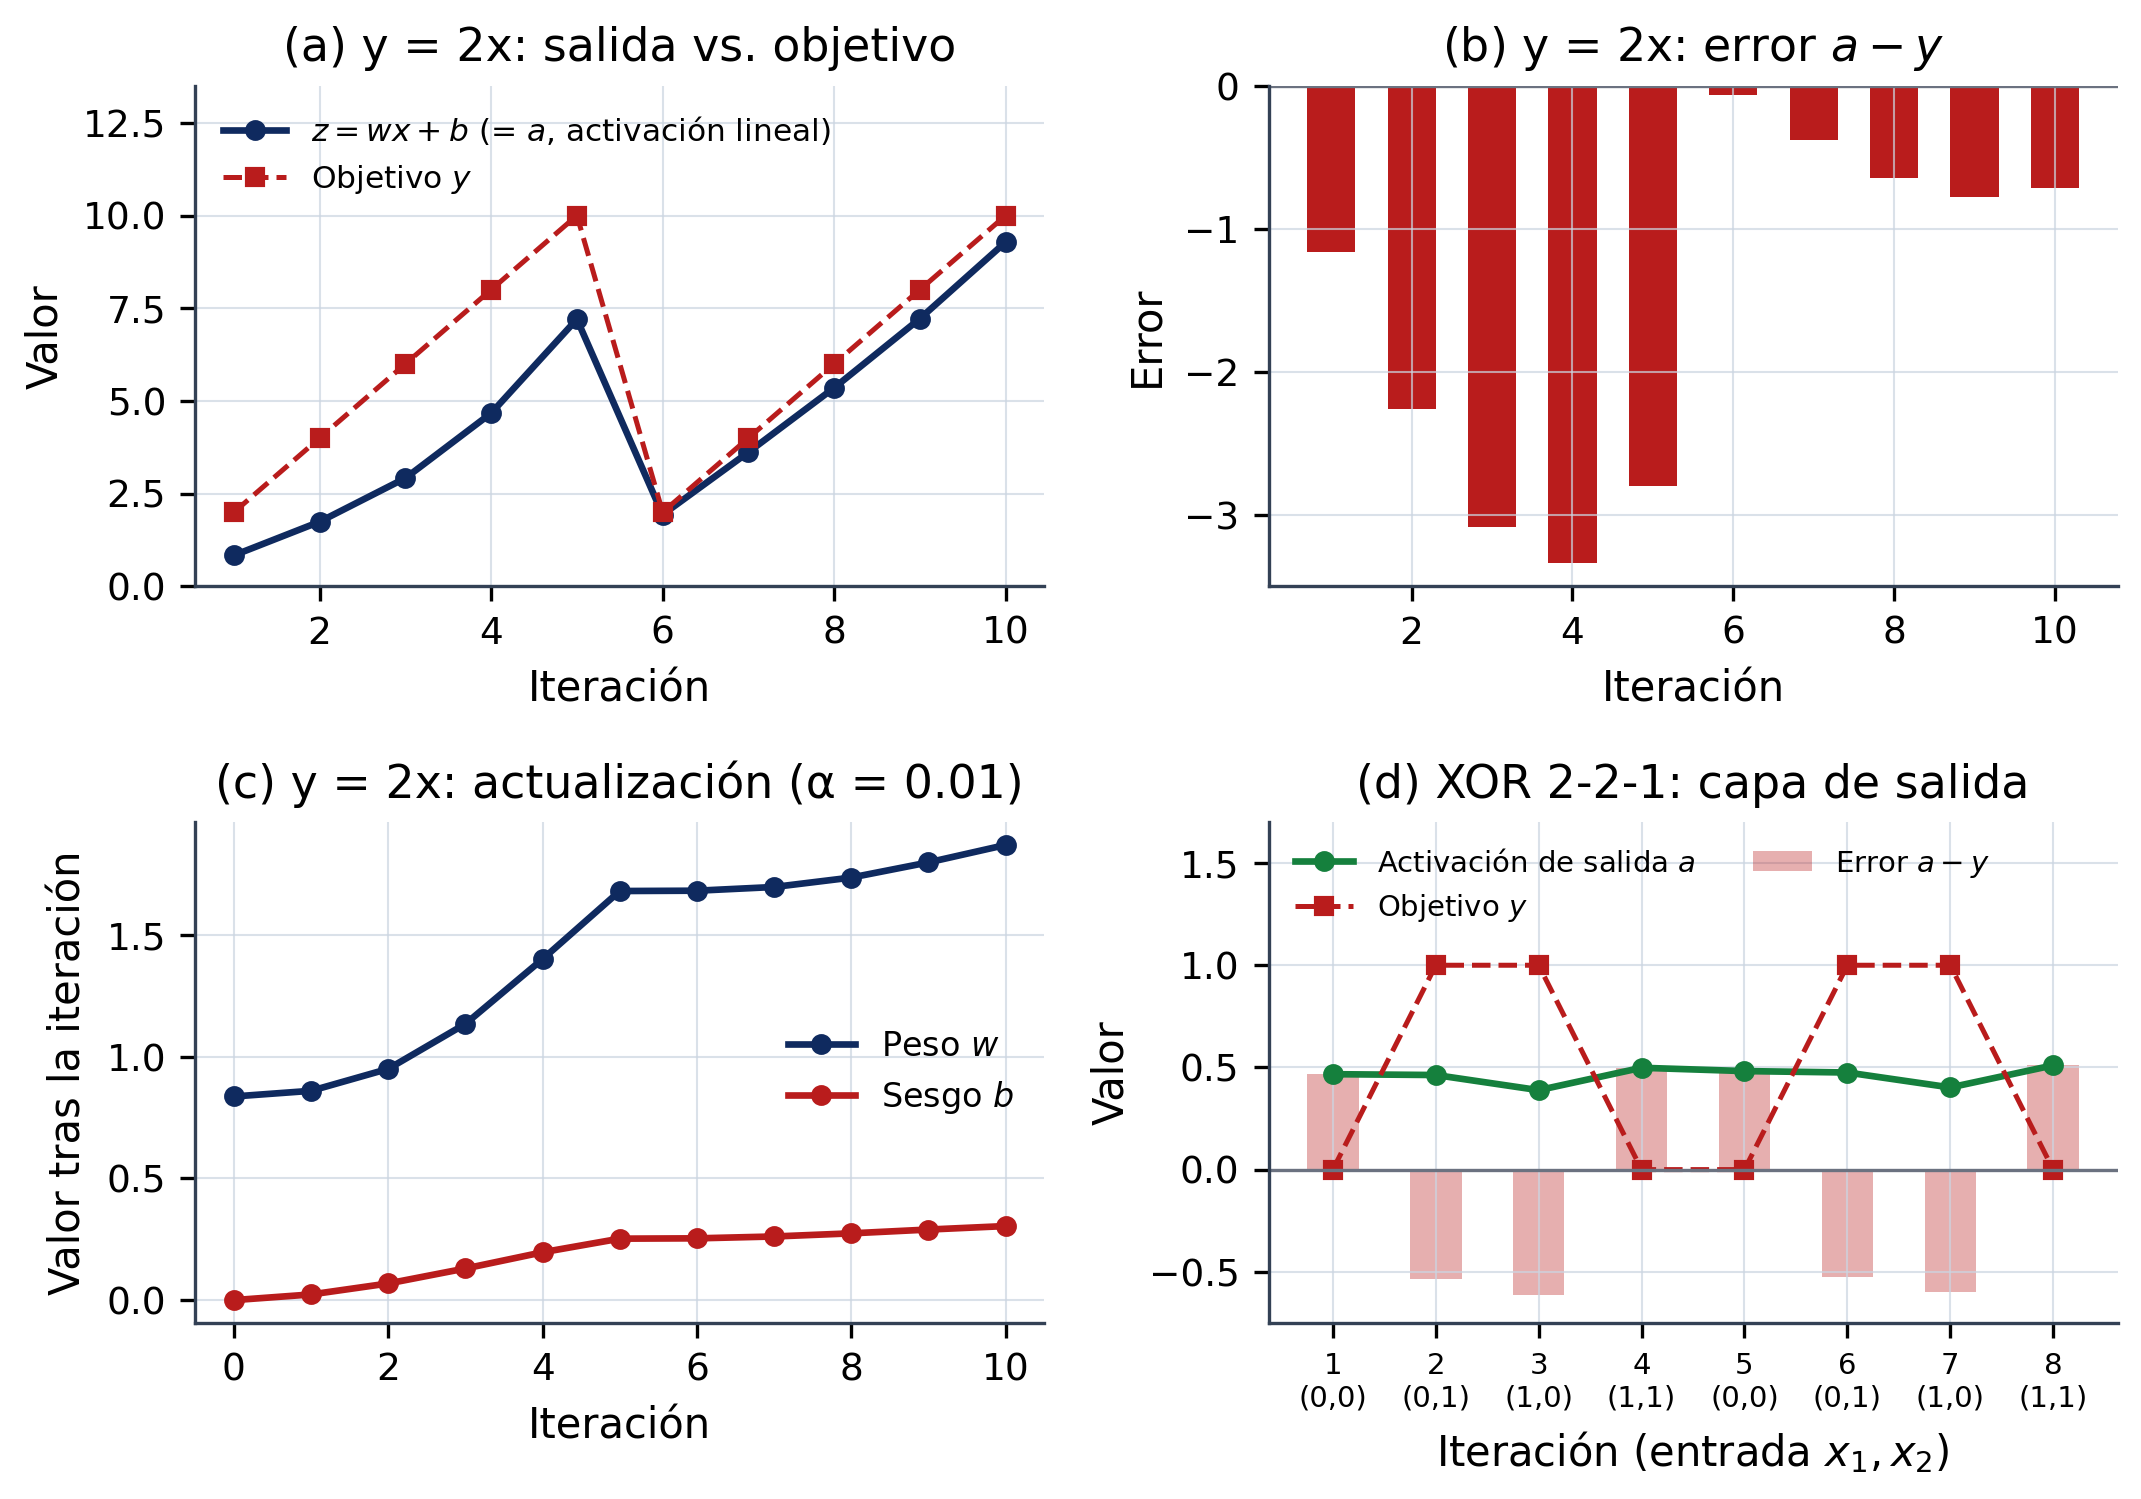
\includegraphics[width=\textwidth]{figuras/fig11_prueba_escritorio.png}
\fuente{Valores de la traza registrada por el binario en \path{resultados/prueba_escritorio.csv}.}
\end{figure}

La traza también incluye las primeras iteraciones de una red \PeXorEsc{} y contiene \PeFilas{} filas en total. La Tabla~\ref{tab:escritorio-xor} muestra las dos primeras iteraciones de esa red. En la primera iteración, la entrada $(0,0)$ anula las sumas ponderadas de la capa oculta, cuyas neuronas producen exactamente $\sigma(0)=0.5$; por ello sus gradientes de pesos son nulos y solo se actualizan los sesgos, comportamiento que coincide con la Ecuación~\eqref{eq:gradW}, pues $\partial\mathcal{L}/\partial w_{ji} = \delta_j\,x_i = 0$ cuando $x_i=0$.

\begin{table}[!htbp]
\caption{Prueba de escritorio de la red XOR 2-2-1 (dos primeras iteraciones)}\label{tab:escritorio-xor}
\footnotesize\setlength{\tabcolsep}{3.5pt}
\begin{tabular*}{\textwidth}{@{\extracolsep{\fill}}rlrrrrrrrr@{}}
\toprule
It. & Entrada & $y$ & Capa & Neurona & $z$ & $a$ & $\delta$ & $b$ & $b'$ \\
\midrule
\TablaEscritorioXor
\bottomrule
\end{tabular*}
\fuente{Capa 1: oculta; capa 2: salida. $\alpha = 0.5$. Fuente: \path{resultados/prueba_escritorio.csv}.}
\end{table}

\subsection{Regresión $y=2x$ en doble precisión}\label{sec:exp1}
El motor complementario repite la regresión con 5 pares $(x,2x)$, peso inicial aleatorio $w_0=\EunoPesoIni$, $\alpha=\EunoAlpha$ y \EunoEpocas{} épocas de descenso de gradiente por muestra. Termina con $w=\EunoPesoFin$ y un MSE de \EunoMseFin, frente a \OfLinMseFin{} del repositorio oficial. La diferencia de cinco órdenes de magnitud se debe al tipo numérico: con \texttt{f64} el error puede descender hasta cerca de $10^{-18}$, mientras que \texttt{f32} representa unas siete cifras decimales y el repositorio oficial se detiene, además, al alcanzar su meta de $10^{-12}$. Ambas implementaciones llegan a la solución analítica $w=2$, $b=0$.

\subsection{Compuerta XOR: necesidad de una capa oculta}\label{sec:exp2}
El repositorio oficial no incluye XOR; el motor complementario lo aborda porque reproduce el problema que detuvo la investigación en redes neuronales durante la década de 1970. La función XOR devuelve 1 cuando sus dos entradas binarias son distintas. Se comparan un perceptrón de una capa (2-1, Sigmoid) y una red multicapa 2-4-1 (Sigmoid/Sigmoid), ambos entrenados durante \EdosEpocas{} épocas con $\alpha=\EdosAlpha$. Además, la red 2-4-1 se entrena con tres tasas de aprendizaje: baja ($0.01$), óptima ($0.5$) y alta ($50$).

\subsubsection*{Perceptrón frente a red multicapa}
El perceptrón terminó con MSE de \EdosMsePer{} y exactitud de \EdosAccPer, mientras que la red multicapa alcanzó MSE de \EdosMseMul{} y exactitud de \EdosAccMul{}. La Tabla~\ref{tab:exp2} presenta las predicciones finales y la Figura~\ref{fig:exp2conv} compara las curvas de pérdida.

\begin{table}[!htbp]
\caption{Predicciones finales para XOR}\label{tab:exp2}
\small
\begin{tabular*}{\textwidth}{@{\extracolsep{\fill}}lrrr@{}}
\toprule
Entrada & Objetivo & Perceptrón 2-1 & Multicapa 2-4-1 \\
\midrule
\TablaEdos
\bottomrule
\end{tabular*}
\fuente{Se clasifica como 1 cuando la salida es $\ge 0.5$. Fuente: \path{resultados/exp2_xor.csv}.}
\end{table}

\begin{figure}[!htbp]
\caption{Curvas de pérdida del perceptrón 2-1 y de la red multicapa 2-4-1 en XOR}\label{fig:exp2conv}
\centering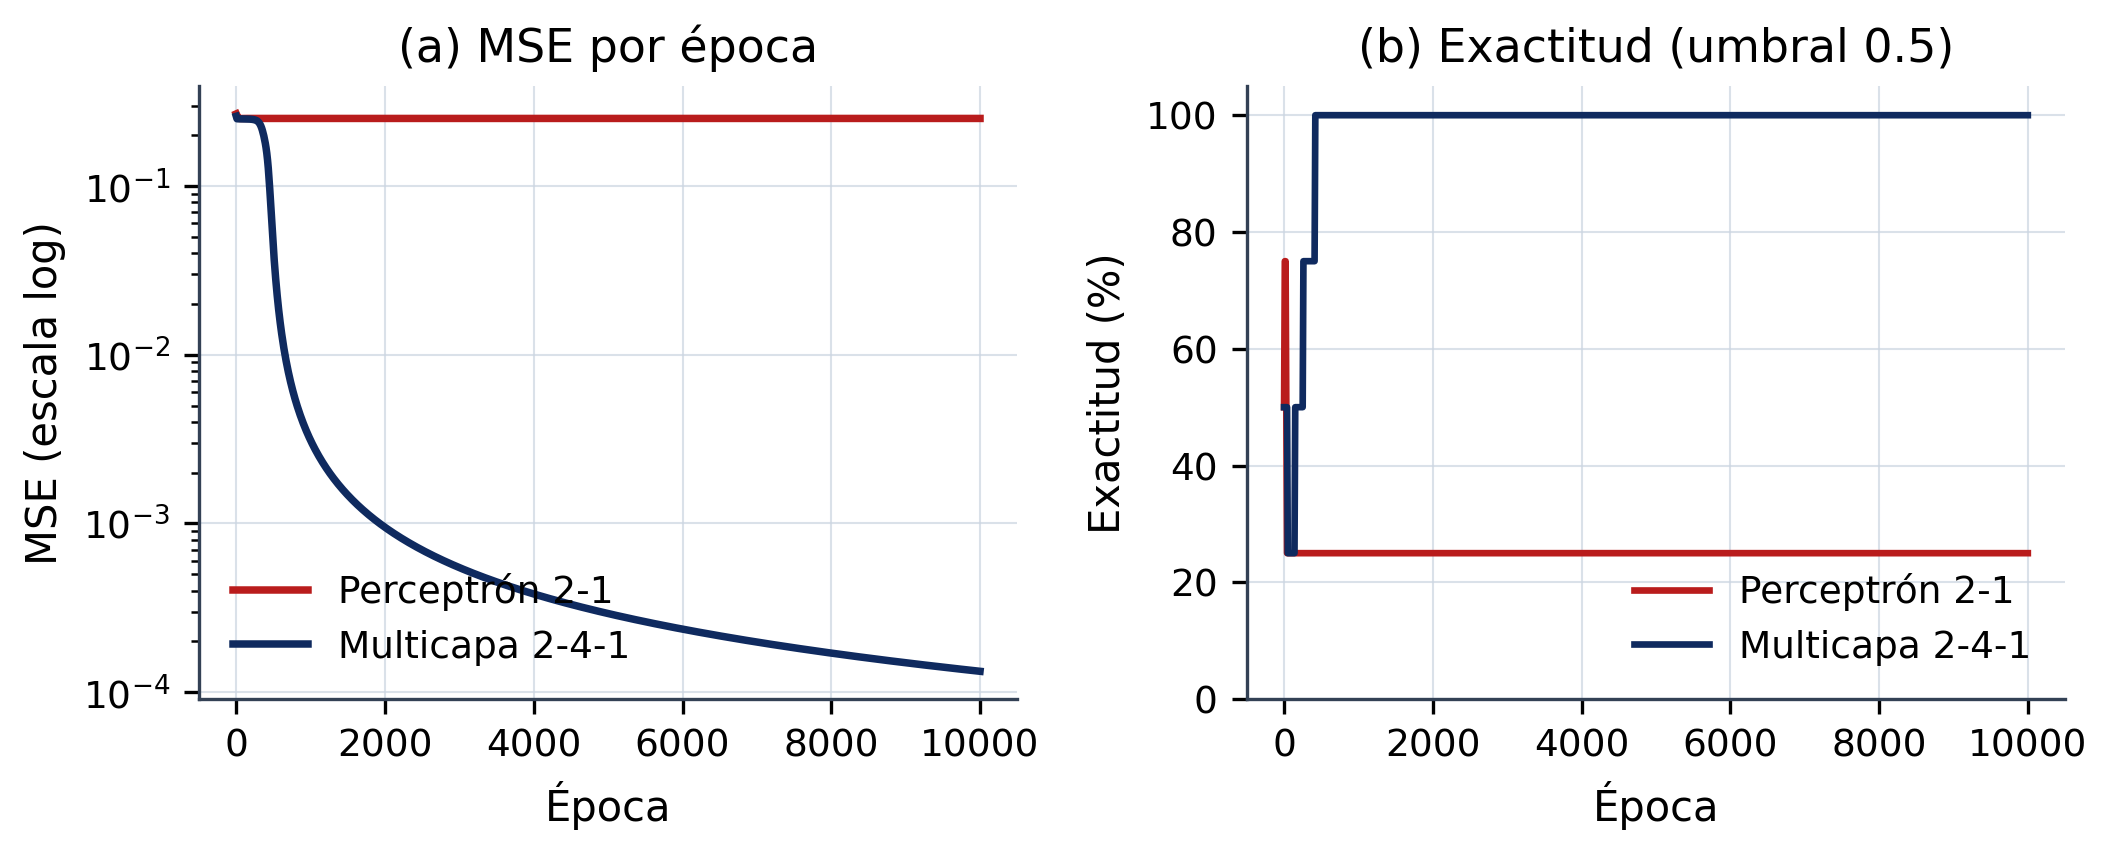
\includegraphics[width=\textwidth]{figuras/fig04_exp2_xor_convergencia.png}
\fuente{Eje vertical en escala logarítmica. Fuente: \path{resultados/exp2_xor.csv}.}
\end{figure}

La Figura~\ref{fig:frontera} muestra la salida de ambos modelos sobre una malla del plano de entradas. El perceptrón solo puede trazar una frontera recta, que deja necesariamente a un punto de cada clase del lado equivocado; la red multicapa, en cambio, construye una región de decisión no lineal que separa correctamente las cuatro entradas.

\begin{figure}[!htbp]
\caption{Fronteras de decisión aprendidas para XOR}\label{fig:frontera}
\centering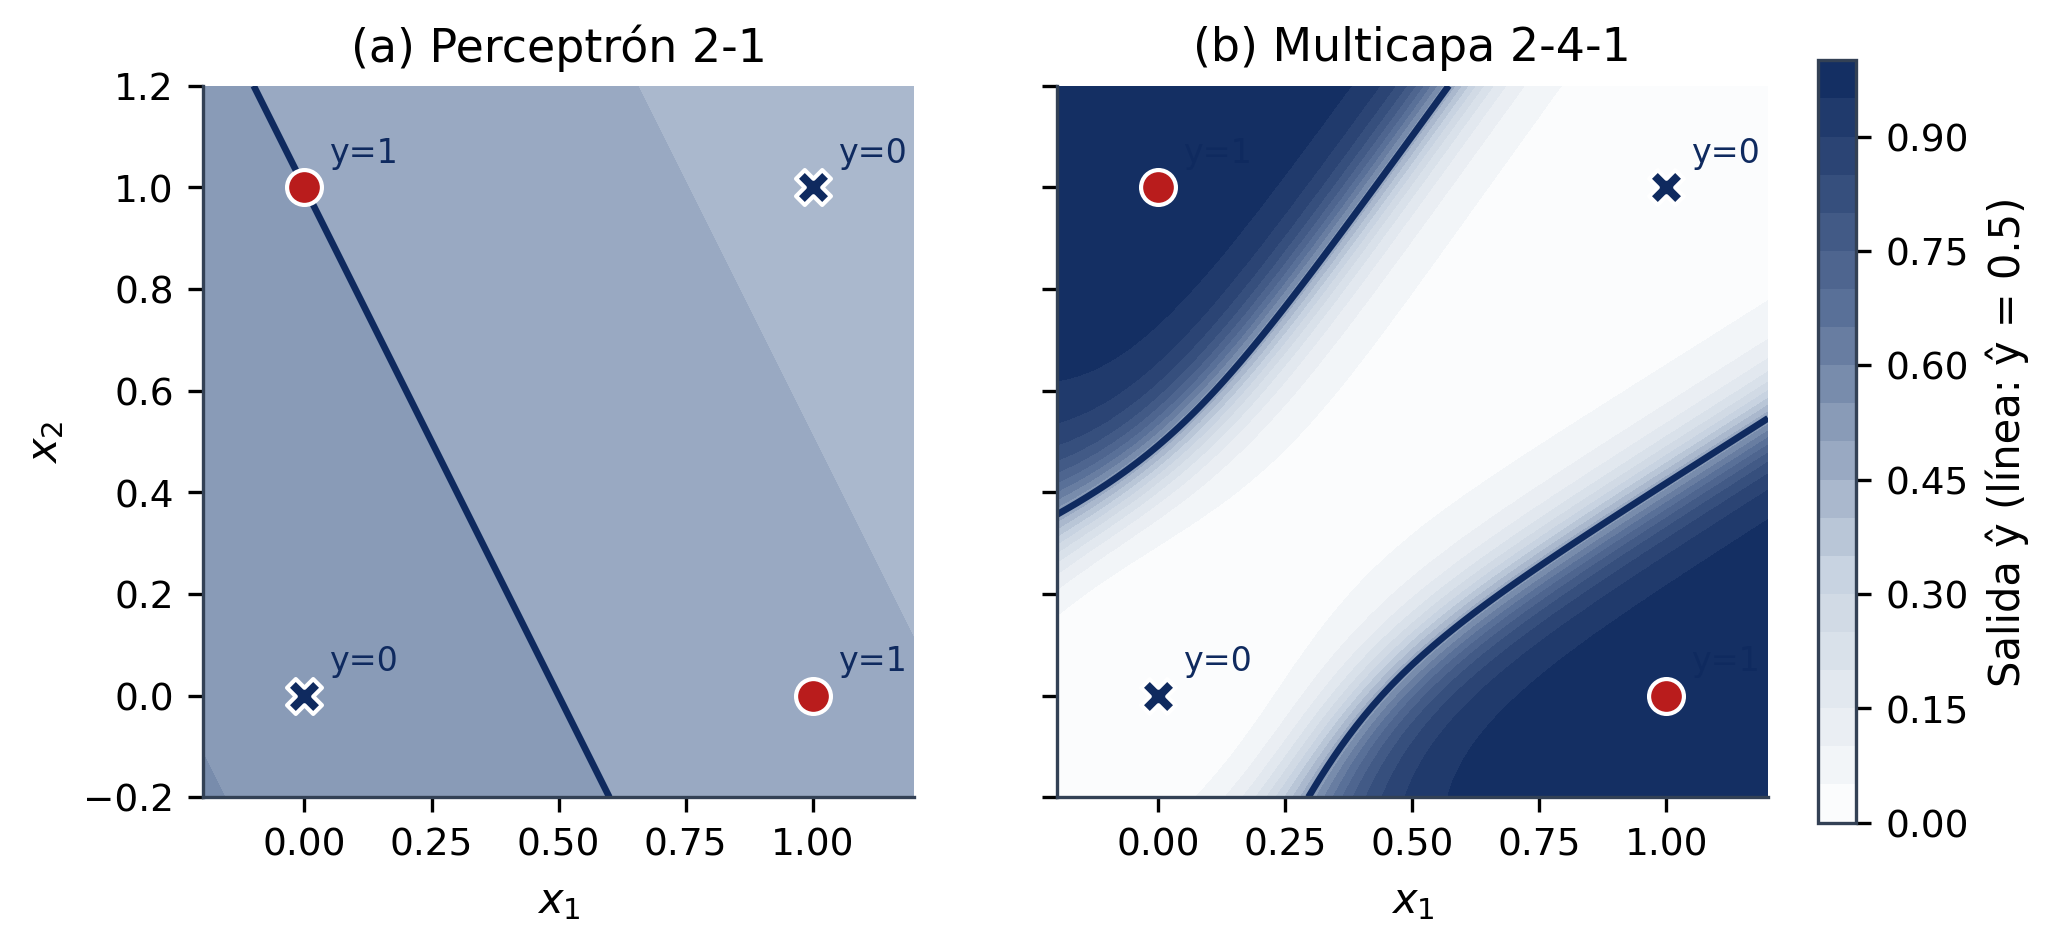
\includegraphics[width=\textwidth]{figuras/fig06_exp2_xor_frontera.png}
\fuente{(a) Perceptrón 2-1. (b) Red multicapa 2-4-1. La línea indica $\hat{y}=0.5$. Fuente: \path{resultados/exp2_xor_frontera.csv}.}
\end{figure}

\subsubsection*{Efecto de la tasa de aprendizaje}
La Tabla~\ref{tab:exp2lr} y la Figura~\ref{fig:lr} resumen el comportamiento de la red 2-4-1 con las tres tasas de aprendizaje estudiadas.

\begin{table}[!htbp]
\caption{Efecto de la tasa de aprendizaje en la red 2-4-1 para XOR}\label{tab:exp2lr}
\small
\begin{tabular*}{\textwidth}{@{\extracolsep{\fill}}lrrrl@{}}
\toprule
Escenario & $\alpha$ & MSE final & Exactitud & Época de convergencia \\
\midrule
\TablaEdosLr
\bottomrule
\end{tabular*}
\fuente{Convergencia: primera época con MSE $<0.01$. Fuente: \path{resultados/exp2_xor_lr.csv}.}
\end{table}

\begin{figure}[!htbp]
\caption{Curvas de pérdida de la red 2-4-1 con tasas de aprendizaje baja, óptima y alta}\label{fig:lr}
\centering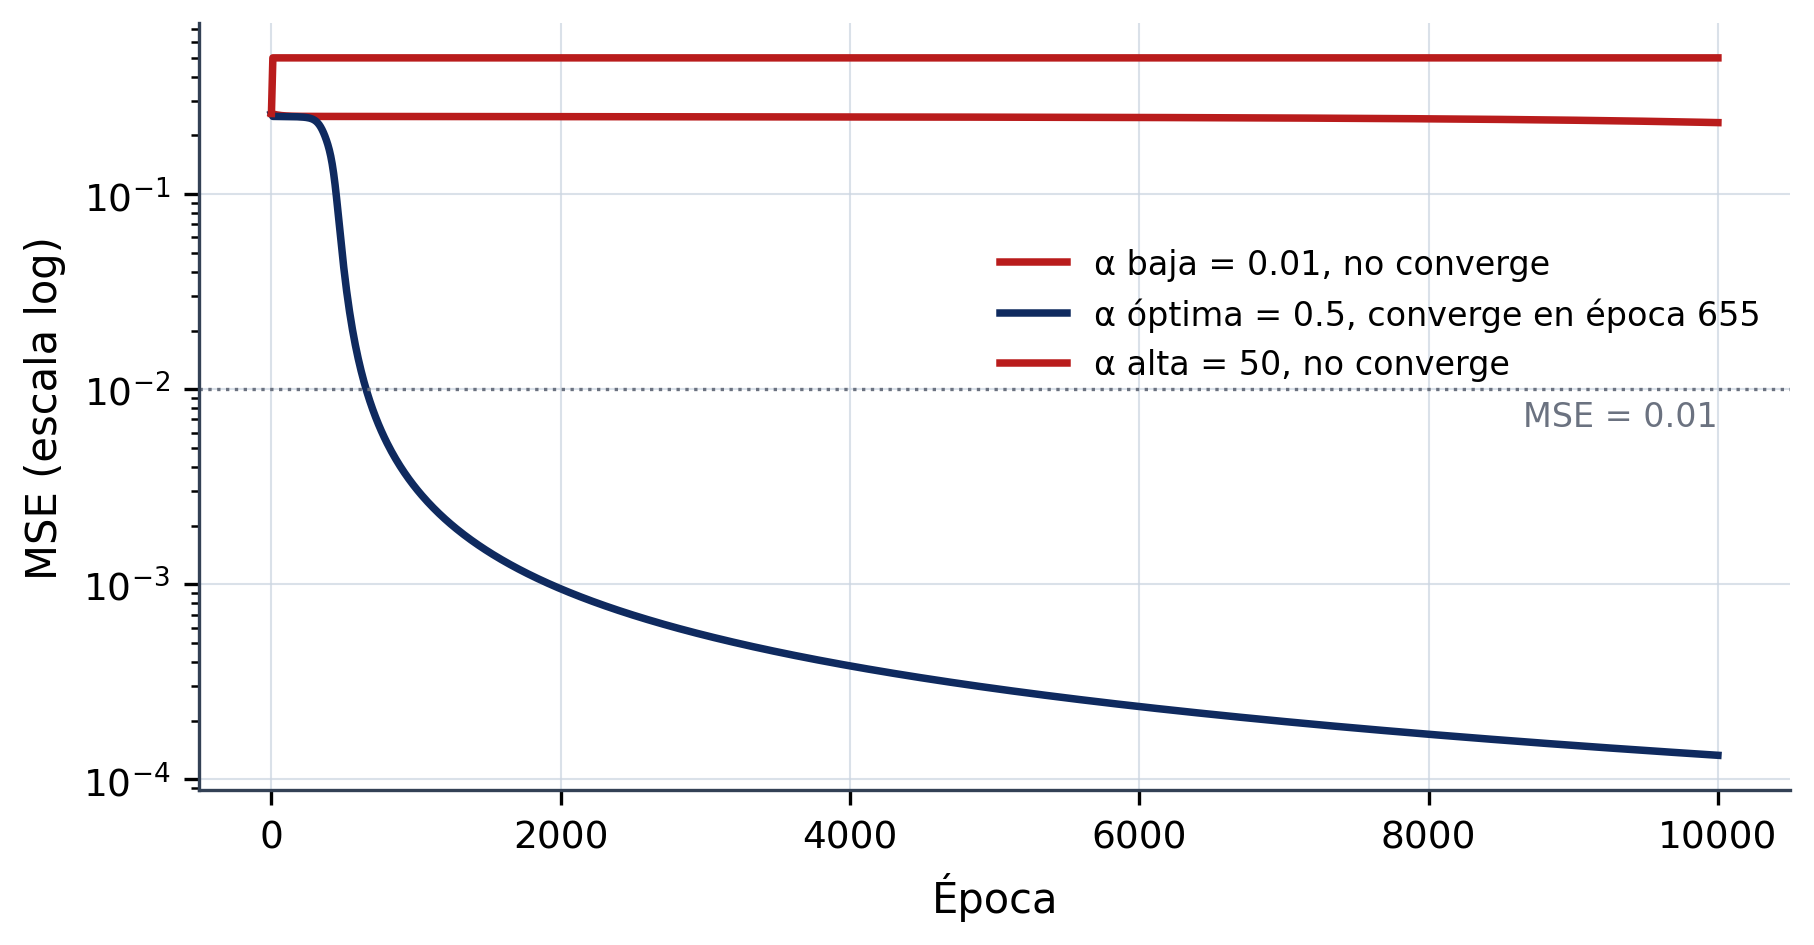
\includegraphics[width=\textwidth]{figuras/fig05_exp2_xor_learning_rates.png}
\fuente{Fuente: \path{resultados/exp2_xor_lr.csv}.}
\end{figure}

\subsubsection*{Análisis}
El perceptrón no puede resolver XOR porque sus cuatro puntos no son linealmente separables, como se demostró en el Capítulo~\ref{cap:marco}. Su MSE se estanca cerca de $0.25$, valor que corresponde a predecir aproximadamente $0.5$ para todas las entradas: el optimizador encuentra el compromiso menos malo entre clases que no puede separar. La capa oculta de la red 2-4-1 transforma el espacio de entrada en una representación en la que las clases sí son separables, lo que confirma empíricamente el teorema de aproximación universal \citep{cybenko1989}.

Respecto a la tasa de aprendizaje, con $\alpha=0.01$ la red apenas avanza en \EdosEpocas{} épocas (MSE de \EdosMseBaja); con $\alpha=0.5$ converge en la época \EdosConvOptima; y con $\alpha=50$ los pasos son tan grandes que las neuronas Sigmoid se saturan, sus derivadas se anulan y el aprendizaje se detiene con MSE de \EdosMseAlta. Este último valor equivale a que la red produzca salidas saturadas en 0 o en 1 que aciertan exactamente la mitad de los casos. El resultado ilustra que la tasa de aprendizaje no es un detalle de configuración, sino un hiperparámetro que determina si el entrenamiento converge \citep{ruder2016}.

\subsection{Vocales con ruido y conjunto de prueba separado}\label{sec:exp3}
El experimento oficial de vocales evalúa los mismos cinco patrones con los que entrena. El motor complementario extiende el problema con una red 25-10-5, variantes ruidosas y un conjunto de prueba separado, lo que permite medir generalización.

\subsubsection*{Conjunto de datos}
Cada vocal se representa como una matriz binaria de $5\times5$ (Figura~\ref{fig:dataset}), aplanada en un vector de 25 entradas. La salida usa codificación \emph{one-hot} de 5 posiciones. El conjunto de entrenamiento contiene \EtresNEnt{} muestras (los 5 prototipos y 4 variantes por vocal con un píxel invertido). El conjunto de prueba contiene \EtresNPru{} muestras distintas de las de entrenamiento: 10 variantes por vocal para cada nivel de ruido de 1 a 5 píxeles invertidos. El ruido se genera invirtiendo $k$ píxeles elegidos mediante el barajado de Fisher--Yates (Código~\ref{cod:ruido}).

\begin{figure}[!htbp]
\caption{Prototipos binarios $5\times5$ y ejemplos con ruido del conjunto de vocales}\label{fig:dataset}
\centering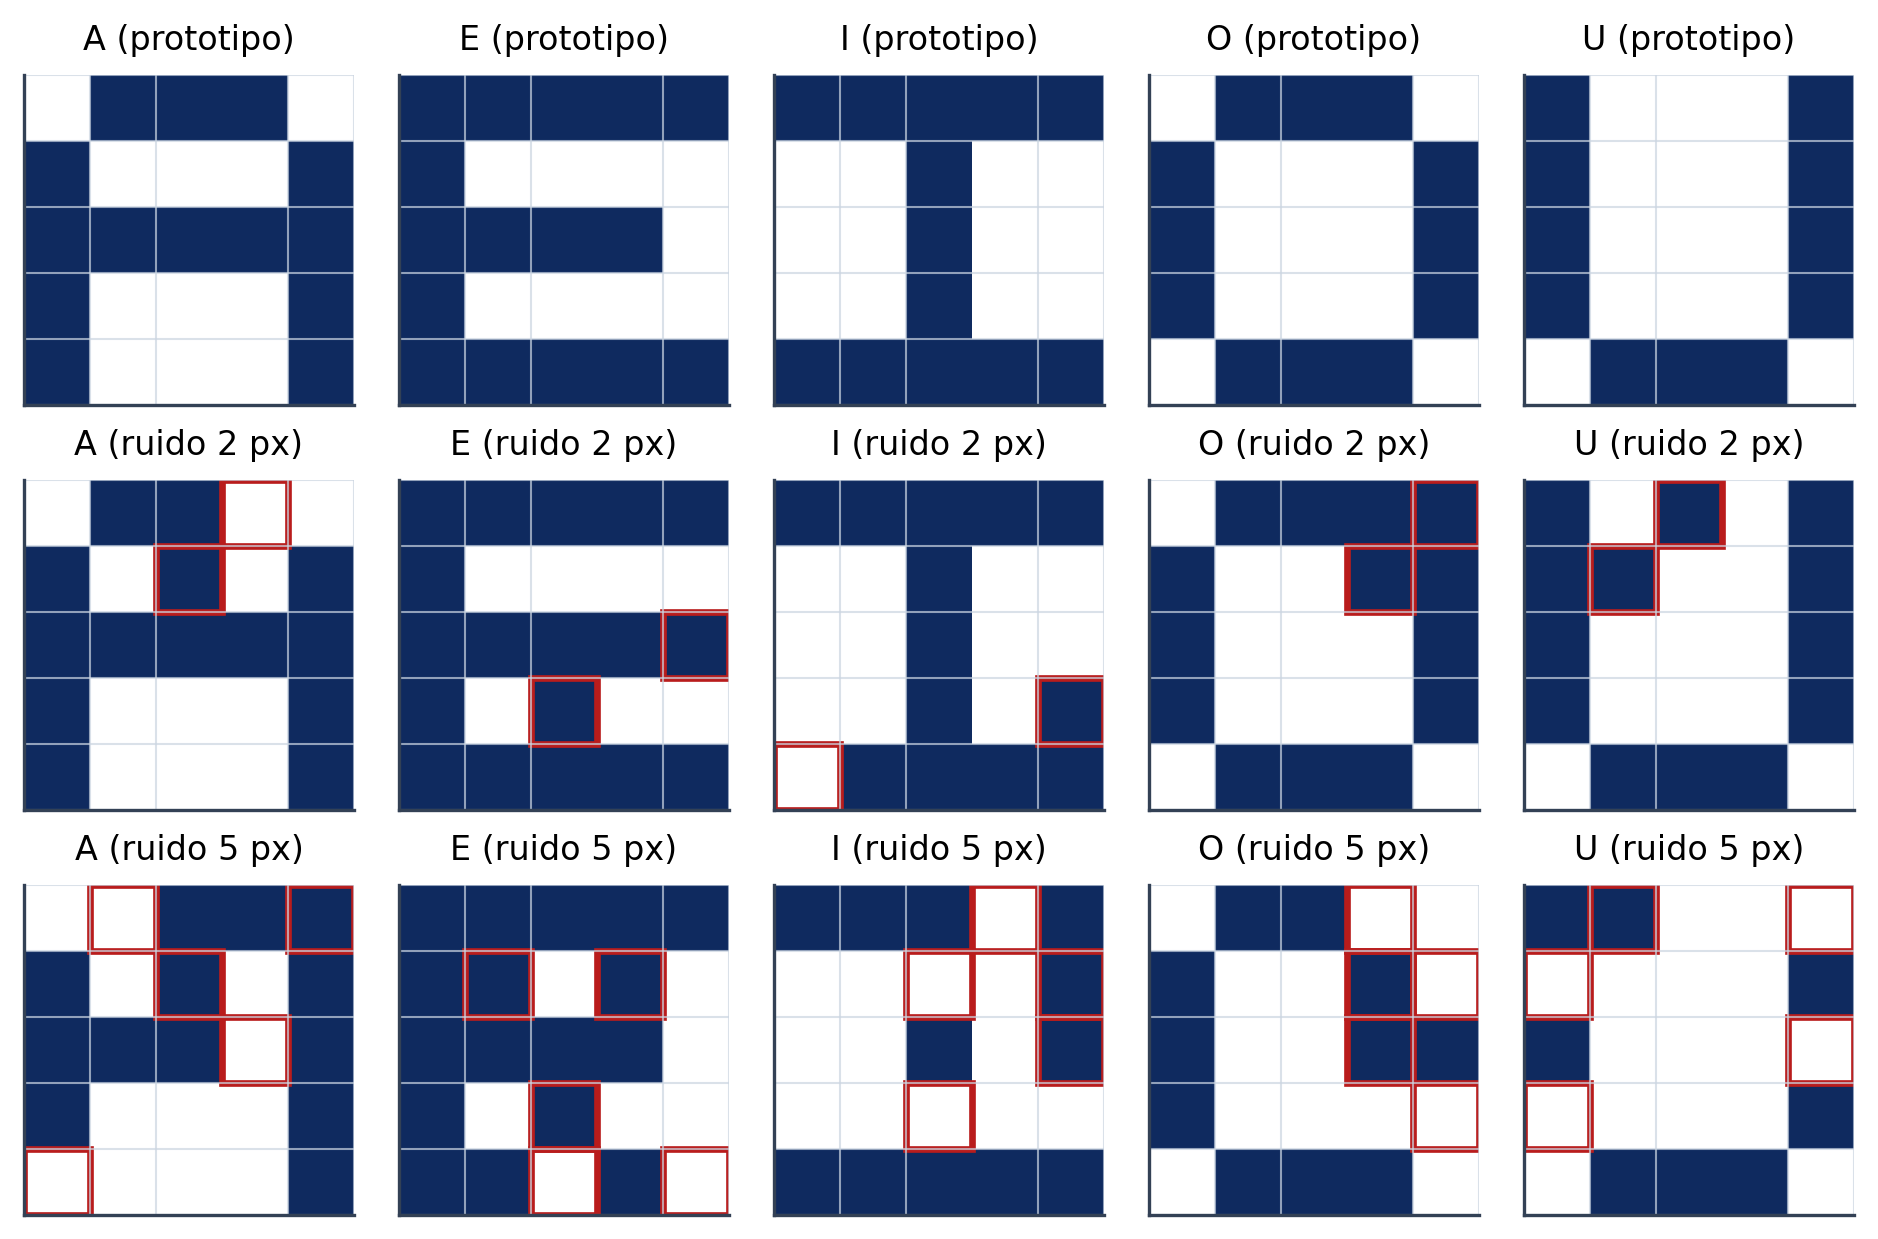
\includegraphics[width=\textwidth,height=0.42\textheight,keepaspectratio]{figuras/fig07_exp3_dataset_vocales.png}
\fuente{Celda oscura = 1, celda clara = 0. Fuente: \path{resultados/dataset_vocales.csv}.}
\end{figure}

\lstinputlisting[caption={Variantes con $k$ píxeles invertidos (\texttt{src/experiments/exp3\_vocales.rs})},label=cod:ruido]{generado/codigo/con_ruido.rs}

\subsubsection*{Resultados}
La red 25-10-5 (Sigmoid/Sigmoid, 315 parámetros) se entrenó durante \EtresEpocas{} épocas con $\alpha=\EtresAlpha$. Alcanzó en entrenamiento un MSE de \EtresMseEnt{} con exactitud de \EtresAccEnt, y en prueba un MSE de \EtresMsePru{} con exactitud de \EtresAccPru. La Figura~\ref{fig:exp3train} muestra la evolución del error, la Tabla~\ref{tab:ruido} desglosa la exactitud por nivel de ruido, y la Tabla~\ref{tab:confusion} y la Figura~\ref{fig:confusion} presentan la matriz de confusión.

\begin{figure}[!htbp]
\caption{Evolución del error de entrenamiento y de prueba en la clasificación de vocales}\label{fig:exp3train}
\centering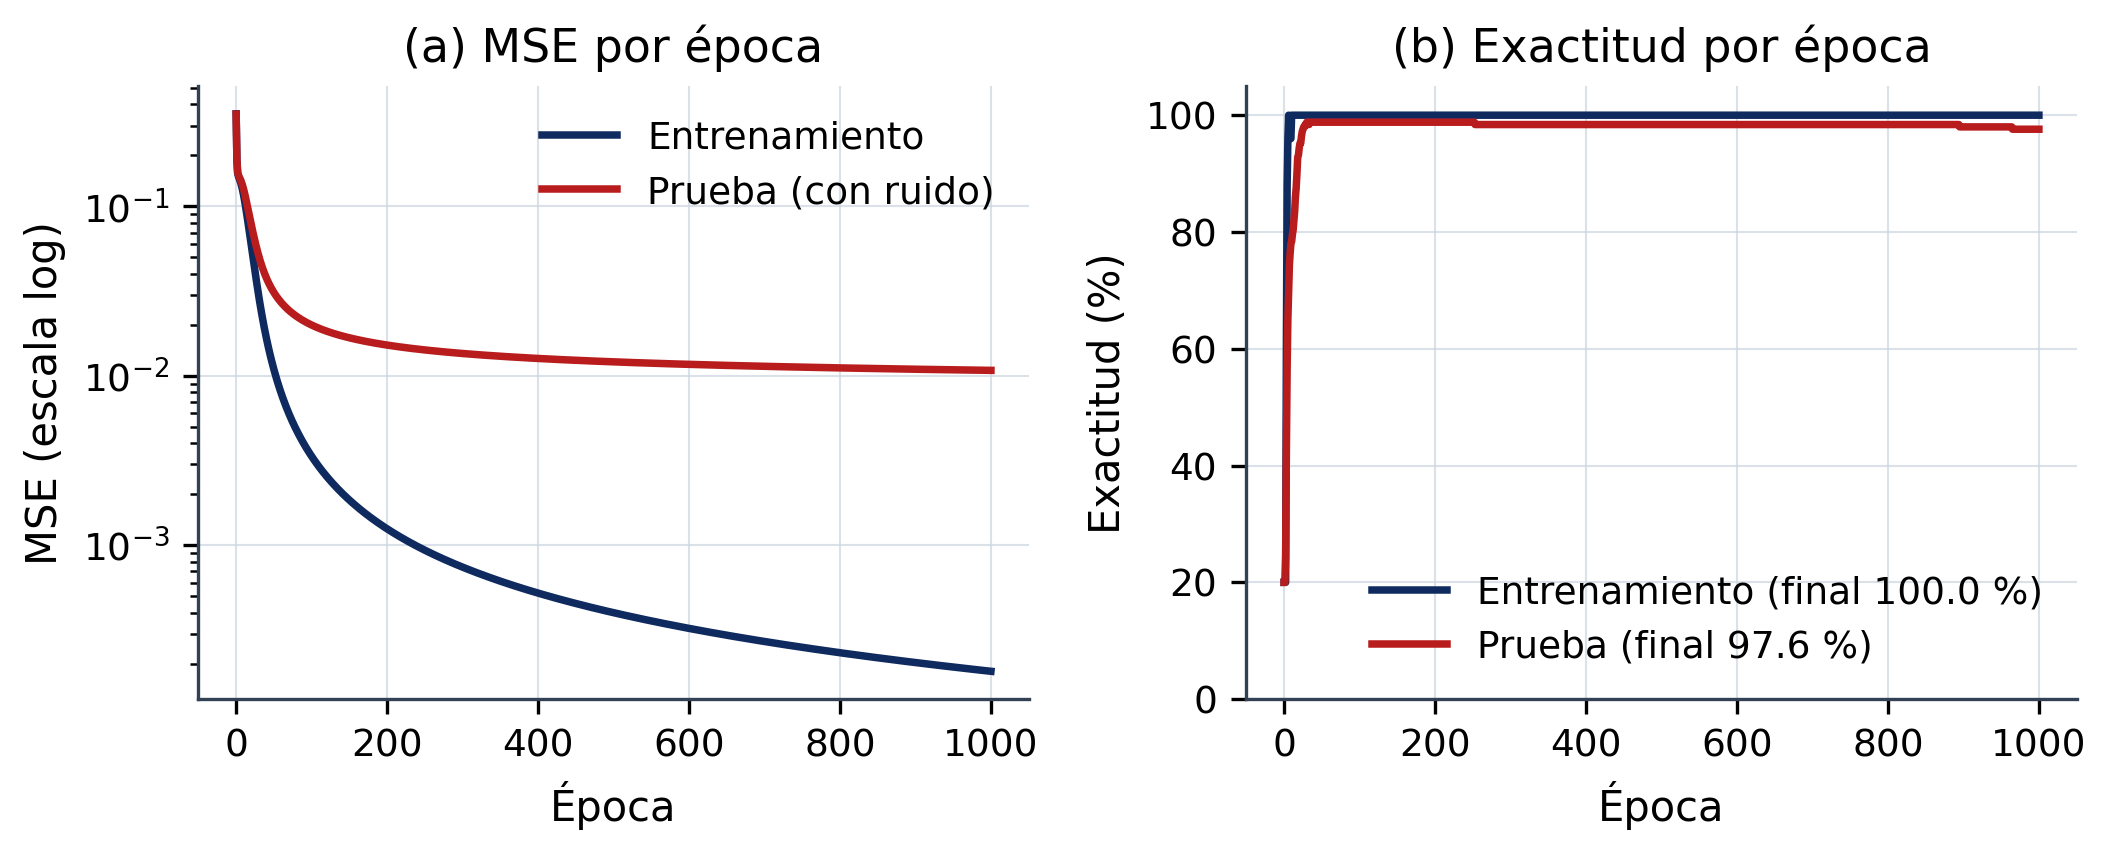
\includegraphics[width=\textwidth]{figuras/fig08_exp3_vocales_entrenamiento.png}
\fuente{Fuente: \path{resultados/exp3_vocales.csv}.}
\end{figure}

\begin{table}[!htbp]
\caption{Exactitud de prueba por nivel de ruido}\label{tab:ruido}
\small
\begin{tabular*}{0.7\textwidth}{@{\extracolsep{\fill}}rrr@{}}
\toprule
Píxeles invertidos & Muestras & Exactitud \\
\midrule
\TablaEtresRuido
\bottomrule
\end{tabular*}
\fuente{Fuente: \path{resultados/resumen.csv}.}
\end{table}

\begin{table}[!htbp]
\caption{Matriz de confusión del conjunto de prueba}\label{tab:confusion}
\small
\begin{tabular*}{0.7\textwidth}{@{\extracolsep{\fill}}l ccccc@{}}
\toprule
Real / Predicha & A & E & I & O & U \\
\midrule
\TablaConfusion
\bottomrule
\end{tabular*}
\fuente{Filas: clase real; columnas: clase predicha. Fuente: \path{resultados/exp3_confusion.csv}.}
\end{table}

\begin{figure}[!htbp]
\caption{Matriz de confusión del Experimento 3}\label{fig:confusion}
\centering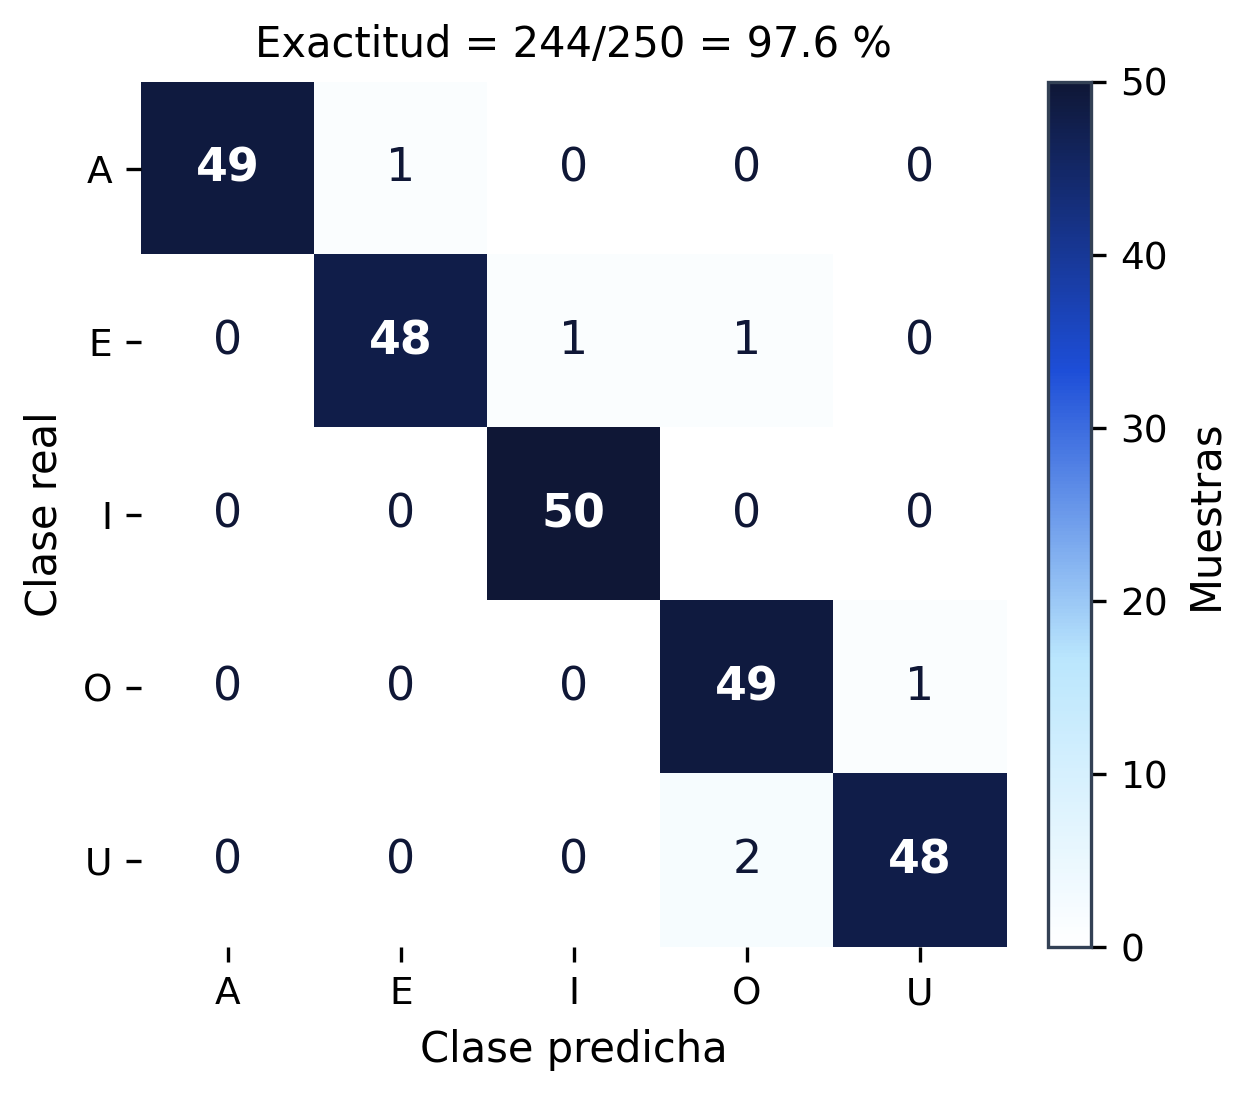
\includegraphics[width=0.72\textwidth]{figuras/fig09_exp3_matriz_confusion.png}
\fuente{La diagonal concentra las clasificaciones correctas. Fuente: \path{resultados/exp3_confusion.csv}.}
\end{figure}

\subsubsection*{Análisis}
La red clasifica sin errores todas las muestras con hasta 3 píxeles invertidos (12\,\% de la imagen), aunque durante el entrenamiento solo vio variantes con un píxel alterado. Con 4 y 5 píxeles invertidos (16\,\% y 20\,\%) la exactitud desciende al 94\,\%. Los errores se concentran entre pares de vocales visualmente parecidas: O y U comparten los laterales y la base, y E comparte la columna izquierda con otras letras. La subsección siguiente examina cada uno de esos errores. La diferencia entre el MSE de entrenamiento y el de prueba es la esperada al evaluar con niveles de ruido mayores que los de entrenamiento, y no impide una exactitud global de \EtresAccPru. El comportamiento es coherente con la representación aprendida y muestra la capacidad de generalización del modelo frente a perturbaciones no observadas.

\subsubsection*{Análisis de los errores de clasificación}
La matriz de confusión registra 6 errores sobre 250 muestras, todos con 4 o 5 píxeles invertidos: 1 A clasificada como E, 1 E como I, 1 E como O, 1 O como U y 2 U como O. Para explicarlos se calculó la distancia de Hamming entre los prototipos, es decir, el número de píxeles en que difieren dos vocales (Tabla~\ref{tab:hamming}). Cuando una muestra tiene $k$ píxeles invertidos, su distancia al prototipo correcto es $k$, y puede quedar tan cerca de otra vocal como de la propia si los píxeles invertidos coinciden con las posiciones en que ambas difieren.

\begin{table}[!htbp]
\caption{Distancia de Hamming entre los prototipos $5\times5$ de las vocales}\label{tab:hamming}
\small
\begin{tabular*}{0.6\textwidth}{@{\extracolsep{\fill}}l ccccc@{}}
\toprule
Vocal & A & E & I & O & U \\
\midrule
\TablaHamming
\bottomrule
\end{tabular*}
\fuente{Número de píxeles distintos entre prototipos. Calculado desde \path{resultados/dataset_vocales.csv}.}
\end{table}

El par O--U es el más cercano, con solo 5 píxeles de diferencia: ambas vocales comparten las columnas laterales y la base redondeada, y se distinguen únicamente por la fila superior. Con 5 píxeles invertidos en esas posiciones, una O puede convertirse exactamente en una U, lo que explica que este par concentre la mitad de los errores (3 de 6). El par E--I, a 7 píxeles, comparte las filas superior e inferior completas, de modo que perder píxeles de la columna izquierda de la E la aproxima a la I. La confusión A--E (8 píxeles) se explica porque ambas comparten la columna izquierda y la barra horizontal central, y la confusión E--O, aunque sus prototipos difieren en 10 píxeles, ocurre porque comparten la columna izquierda y el ruido elimina los extremos horizontales que caracterizan a la E. La I, la vocal más distante de las demás, no registra ningún error. El análisis confirma que los errores no son aleatorios, sino que siguen la geometría del conjunto de datos: a menor distancia de Hamming entre prototipos, mayor probabilidad de confusión con ruido elevado.

\subsection{Rendimiento y benchmarks}\label{sec:bench}
Los tiempos se midieron con \texttt{std::time::Instant} sobre el binario compilado en modo \emph{release} (sistema \BenchSO, arquitectura \BenchArch), como promedio de 3 repeticiones; la inferencia se promedió sobre 100\,000 predicciones. El binario resultante ocupa \BinKiB~KiB. La Tabla~\ref{tab:bench} presenta los valores medidos y la Figura~\ref{fig:bench} su representación gráfica.

\begin{table}[!htbp]
\caption{Tiempos reales de entrenamiento e inferencia}\label{tab:bench}
\small
\begin{tabular*}{\textwidth}{@{\extracolsep{\fill}}llrrrrr@{}}
\toprule
Experimento & Red & Parám. & Épocas & Entren. (ms) & µs/época & Inferencia (ns) \\
\midrule
\TablaBench
\bottomrule
\end{tabular*}
\fuente{Los tiempos dependen del equipo utilizado. Fuente: \path{resultados/benchmarks.csv}.}
\end{table}

\begin{figure}[!htbp]
\caption{Tiempos de entrenamiento e inferencia del motor en Rust}\label{fig:bench}
\centering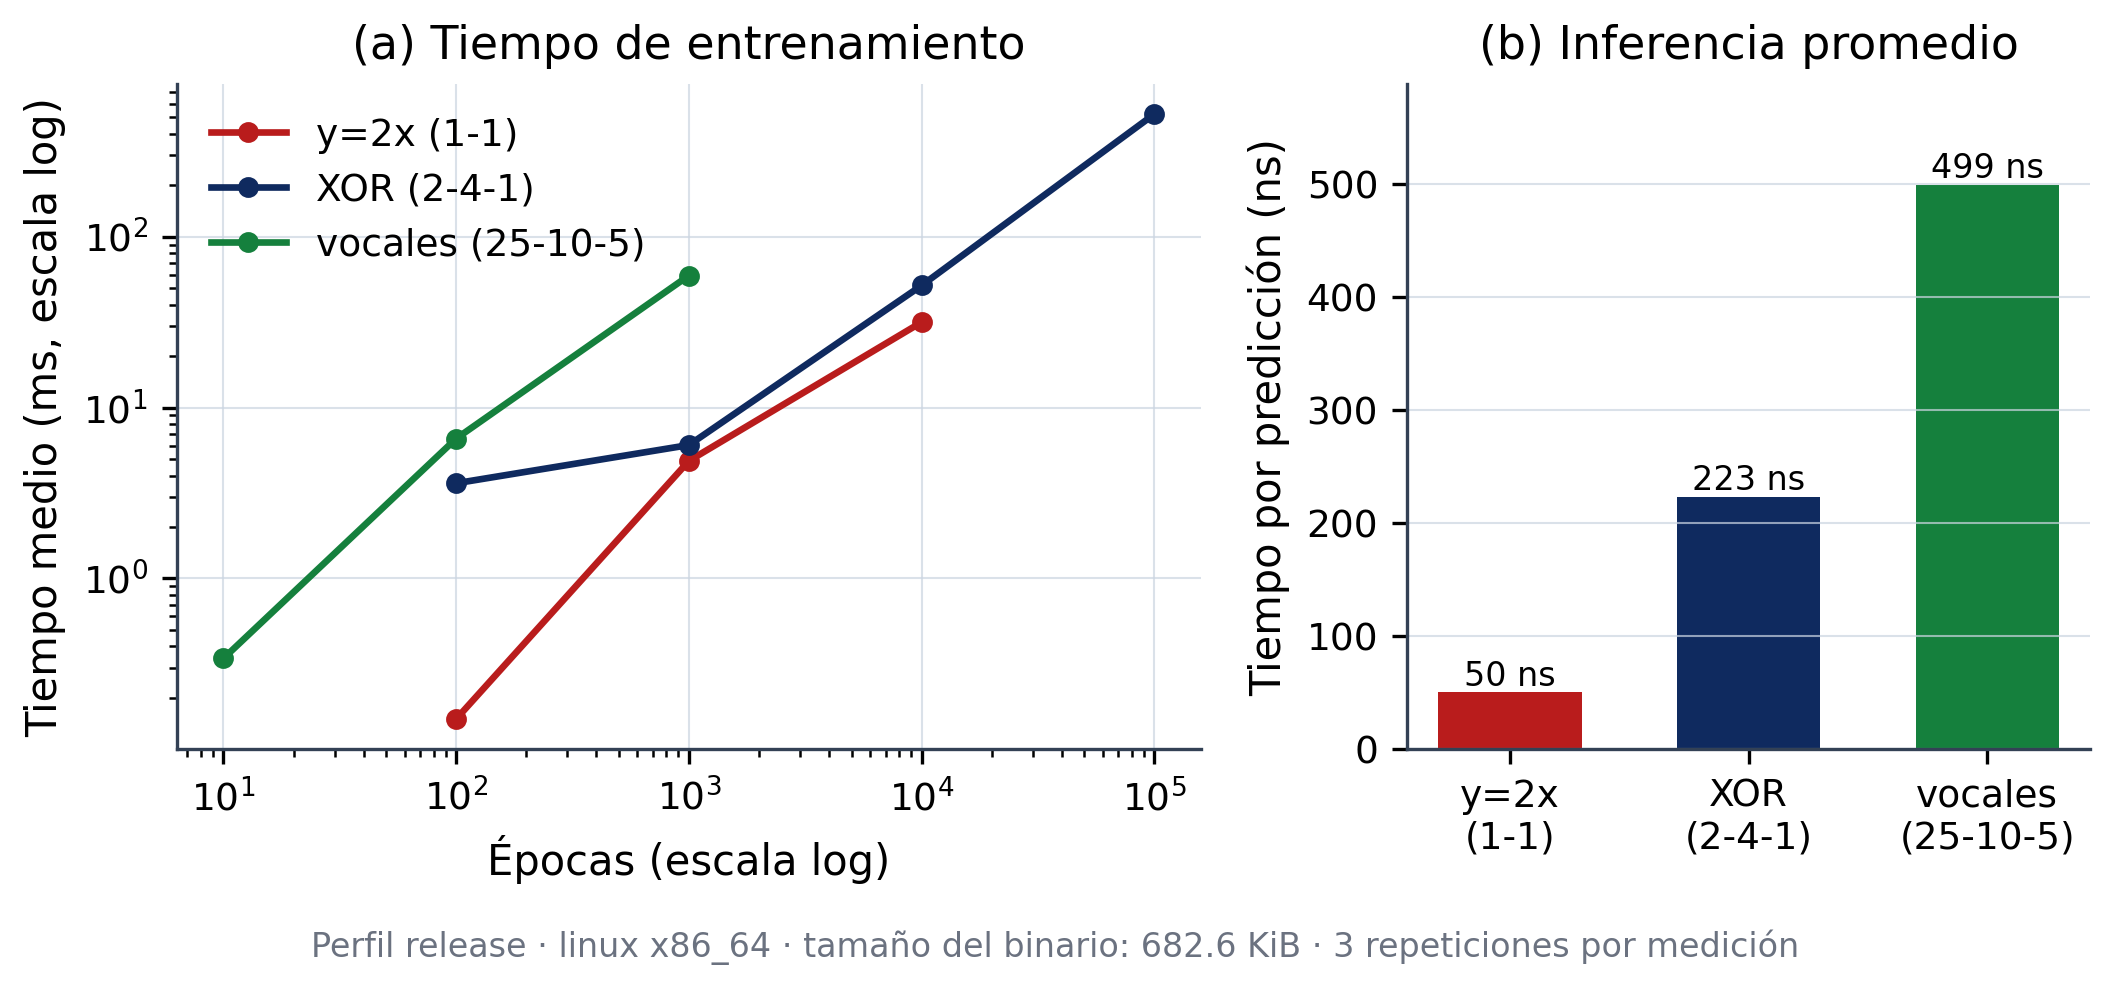
\includegraphics[width=\textwidth]{figuras/fig10_benchmarks_rust.png}
\fuente{(a) Tiempo medio de entrenamiento según el número de épocas, en escala logarítmica. (b) Tiempo medio por predicción. Fuente: \path{resultados/benchmarks.csv}.}
\end{figure}

El costo por época se mantiene aproximadamente constante para cada arquitectura una vez superadas las primeras ejecuciones, en las que influyen efectos de calentamiento de la caché, lo que confirma la complejidad lineal $O(E\cdot N\cdot P)$ del entrenamiento. La inferencia crece con el número de parámetros: la red de vocales, con 315 parámetros, requiere más tiempo por predicción que la red XOR de 17 parámetros, y ambas operan en el orden de los cientos de nanosegundos. Incluso 100\,000 épocas de XOR se completan en menos de un segundo, lo que demuestra que no se requiere hardware especializado para estudiar estos fundamentos.

\chapter{Guía de Instalación, Uso y Demostración}\label{cap:guia}
Este capítulo constituye el manual de usuario del proyecto. Describe los requisitos del entorno, la instalación de las herramientas, la compilación y ejecución del repositorio oficial, el uso del motor complementario, la regeneración de los resultados y de este documento, y el guion recomendado para la demostración en la Feria Facultativa. Los comandos se presentan para un sistema GNU/Linux; en Windows y macOS son idénticos una vez instalado Rust.

\section{Requisitos del entorno}
El repositorio oficial solo requiere el compilador de Rust y su gestor Cargo. Las herramientas de documentación son opcionales y solo se necesitan para regenerar las gráficas y este documento. La Tabla~\ref{tab:requisitos} resume el software utilizado.

\begin{table}[!htbp]
\caption{Software requerido y opcional}\label{tab:requisitos}
\small
\begin{tabularx}{\textwidth}{@{}l l >{\raggedright\arraybackslash}X@{}}
\toprule
Herramienta & Uso & Necesidad \\
\midrule
Rust y Cargo (edición 2024) & Compilar y ejecutar el repositorio & Obligatoria \\
Git & Clonar el repositorio & Recomendada \\
Python 3 con \texttt{matplotlib} & Generar gráficas desde los CSV & Opcional (documentación) \\
TeX Live con XeLaTeX y \texttt{latexmk} & Compilar el PDF del documento & Opcional (documentación) \\
Pandoc y \texttt{python-docx} & Generar la versión DOCX editable & Opcional (documentación) \\
draw.io (diagrams.net) & Editar y exportar los diagramas & Opcional (documentación) \\
\bottomrule
\end{tabularx}
\fuente{Todas las herramientas son gratuitas y de código abierto. No se requiere GPU; la primera compilación descarga el crate \texttt{rand} desde crates.io.}
\end{table}

\section{Instalación}
Rust se instala con el instalador oficial \texttt{rustup}, que descarga el compilador, Cargo y la biblioteca estándar. A continuación se clona el repositorio oficial y se compila en modo optimizado.

\begin{lstlisting}[language={},numbers=none,caption={Instalación de Rust y obtención del repositorio oficial},label=cod:instalacion]
curl --proto '=https' --tlsv1.2 -sSf https://sh.rustup.rs | sh
source "$HOME/.cargo/env"
rustc --version && cargo --version
git clone https://github.com/lanorrron/neural-network.git
cd neural-network
cargo build --release
\end{lstlisting}

El archivo \texttt{Cargo.toml} declara una sola dependencia, \texttt{rand 0.9}, que Cargo descarga junto con sus dependencias transitivas en la primera compilación; después puede trabajarse sin conexión. Ningún crate de aprendizaje automático ni de álgebra lineal interviene en el proyecto.

\section{Ejecución de los experimentos}
El binario recibe como argumento el experimento que se desea ejecutar. La Tabla~\ref{tab:cli} describe las órdenes disponibles, definidas en \texttt{src/main.rs} (Código~\ref{cod:main}).

\begin{table}[!htbp]
\caption{Órdenes de la interfaz de línea de comandos del repositorio oficial}\label{tab:cli}
\small
\begin{tabularx}{\textwidth}{@{}l >{\raggedright\arraybackslash}X@{}}
\toprule
Orden & Efecto \\
\midrule
\texttt{cargo run} & Entrena la red de vocales e informa las cinco predicciones \\
\texttt{cargo run -- lineal} & Regresión $y=2x$ con una neurona lineal \\
\texttt{cargo run -- booleano} & Clasificación de 0 como falso y 1 como verdadero \\
\texttt{cargo run -- vocal <letra>} & Entrena la red de vocales y evalúa la vocal indicada (A, E, I, O o U) \\
\texttt{cargo run -- <letra>} & Forma abreviada de la orden anterior \\
\bottomrule
\end{tabularx}
\fuente{Una letra no válida produce un mensaje de error. Con \texttt{--release} se usa el binario optimizado.}
\end{table}

\begin{lstlisting}[language={},numbers=none,caption={Ejemplos de ejecución del repositorio oficial},label=cod:ejecucion]
cargo run --release -- lineal       # y = 2x, se detiene al alcanzar MSE <= 1e-12
cargo run --release -- booleano     # 250 epocas con gradientes por epoca
cargo run --release -- vocal a      # entrena y reconoce la vocal A
\end{lstlisting}

Los resultados se imprimen en la terminal; el programa no escribe archivos. Para documentar este trabajo, el script \path{scripts/auditar_repo_oficial.py} del repositorio de documentación compila la instantánea del commit \texttt{\OfCommit} guardada en \path{repo_oficial/neural-network/}, ejecuta las cuatro órdenes, guarda su salida en \path{resultados/oficial/*.txt} y la convierte en los CSV descritos en la Tabla~\ref{tab:csv}.

\begin{table}[!htbp]
\caption{Archivos de resultados de la auditoría del repositorio oficial}\label{tab:csv}
\small
\begin{tabularx}{\textwidth}{@{}l >{\raggedright\arraybackslash}X@{}}
\toprule
Archivo & Contenido \\
\midrule
\texttt{lineal.csv}, \texttt{lineal\_predicciones.csv} & Época, peso, bias y MSE; predicciones finales de $y=2x$ \\
\texttt{booleano.csv}, \texttt{booleano\_predicciones.csv} & Gradientes y parámetros por época; probabilidades finales \\
\texttt{vocales.csv}, \texttt{vocales\_predicciones.csv} & Probabilidad de cada vocal y cambio máximo por informe; predicciones finales \\
\texttt{vocal\_a.csv} & Probabilidades asignadas al evaluar la vocal A \\
\texttt{cargo\_test.txt}, \texttt{cargo\_clippy.txt} & Salida completa de las pruebas y del análisis estático \\
\texttt{resumen.csv} & Métricas finales, tiempos, advertencias y tamaño del binario \\
\bottomrule
\end{tabularx}
\fuente{Directorio \path{resultados/oficial/}. Auditoría completa en \path{docs/auditoria_repo_oficial.md}.}
\end{table}

\section{Verificación y motor complementario}
En el repositorio oficial, \texttt{cargo test} compila el proyecto y ejecuta \OfPruebas{} pruebas, y \texttt{cargo clippy} informa \OfClippyErr{} error (\texttt{modulo\_one}, en \texttt{vowels.rs}, porque \texttt{REPORT\_EVERY} vale 1) y \OfClippyWarn{} advertencias, en su mayoría código definido pero aún no utilizado. La verificación automatizada de las ecuaciones se realiza con el motor complementario, que se obtiene y ejecuta como sigue.

\begin{lstlisting}[language={},numbers=none,caption={Pruebas y experimentos del motor complementario},label=cod:pruebas]
git clone https://github.com/Noxy-bit/Redes-Neuronales-Rust.git
cd Redes-Neuronales-Rust
cargo test                          # 52 pruebas, incluido gradient checking
cargo run --release -- --all        # XOR, vocales con ruido y benchmarks -> resultados/*.csv
\end{lstlisting}

\section{Regeneración de gráficas, diagramas y documento}
Las gráficas, los diagramas y este documento se regeneran a partir de los resultados con los siguientes comandos. El script de compilación extrae los fragmentos de código, genera las macros de resultados desde los CSV, compila el PDF con XeLaTeX y produce la versión DOCX.

\begin{lstlisting}[language={},numbers=none,caption={Regeneración de la documentación},label=cod:regenerar]
python3 scripts/auditar_repo_oficial.py     # ejecuta el repositorio oficial -> resultados/oficial/
python3 scripts/graficas_repo_oficial.py    # 3 graficas oficiales (300 DPI)
python3 scripts/generar_graficas.py         # graficas del motor complementario
python3 diagramas/generar_diagramas.py      # diagramas .drawio -> PNG (requiere draw.io)
bash tesis/compilar_final.sh                # PDF y DOCX en tesis/build/
\end{lstlisting}

\section{Guion de demostración en la feria}
La demostración en el stand está pensada para durar entre cinco y siete minutos y puede adaptarse al tiempo disponible. Se recomienda tener el repositorio oficial compilado previamente y una terminal abierta en su raíz; las pausas del programa permiten seguir el entrenamiento en la pantalla.

\begin{enumerate}[leftmargin=2em,itemsep=4pt]
\item \textbf{Motivación (1 minuto).} Presentar el problema de la caja negra con el árbol de problemas (Figura~\ref{fig:arbol}) y la pregunta de investigación.
\item \textbf{Arquitectura (1 minuto).} Mostrar la Figura~\ref{fig:arquitectura}: vectores, neurona, error, gradiente y descenso de gradiente escritos a mano.
\item \textbf{Regresión en vivo (1 minuto).} Ejecutar \texttt{cargo run --release -- lineal} y observar cómo el peso se acerca a 2 y el MSE desciende hasta $10^{-12}$.
\item \textbf{Vocal elegida por el público (2 minutos).} Pedir a un visitante una vocal, ejecutar \texttt{cargo run --release -- vocal <letra>} y comentar cómo crece la probabilidad de la clase correcta; mostrar los patrones de la Figura~\ref{fig:of-voc}.
\item \textbf{Más allá de una capa (1 minuto).} Con el motor complementario, mostrar la frontera de XOR (Figura~\ref{fig:frontera}) y las pruebas de \emph{gradient checking}.
\item \textbf{Cierre (1 minuto).} Relacionar el proyecto con los contenidos de Programación 1 (Tabla~\ref{tab:inf120}) e invitar a escanear el código QR del repositorio oficial.
\end{enumerate}

\begin{nota}[Preguntas frecuentes del público]
\textbf{¿Por qué no usar Python y una biblioteca?} Porque el objetivo es comprender y verificar cada operación, no solo obtener un resultado. \textbf{¿La red aprende o memoriza?} La demostración de vocales usa un único patrón por letra; el motor complementario evalúa vocales con ruido no vistas en el entrenamiento y alcanza \EtresAccPru{} de exactitud. \textbf{¿Se necesita una computadora potente?} No: el binario oficial ocupa \OfBinKiB~KiB y su cómputo dura milisegundos; la mayor parte del tiempo en pantalla corresponde a las pausas de la demostración.
\end{nota}

\section{Solución de problemas frecuentes}
Si \texttt{cargo} no se reconoce como comando después de la instalación, debe abrirse una nueva terminal o ejecutarse \texttt{source "\$HOME/.cargo/env"}. Si la compilación indica que la edición 2024 no es compatible, debe actualizarse Rust con \texttt{rustup update stable}. Si la primera compilación falla al descargar \texttt{rand}, debe verificarse la conexión a Internet. Las métricas de los experimentos oficiales deben coincidir exactamente en cualquier equipo, porque no intervienen números aleatorios; los tiempos, en cambio, dependen del procesador. Si la generación de gráficas falla, debe instalarse \texttt{matplotlib} con \texttt{pip install matplotlib}.

\chapter{Conclusiones}\label{cap:conclusiones}
A partir de la implementación y de los resultados experimentales reales, se presentan las conclusiones del proyecto organizadas según los objetivos planteados en el Capítulo~\ref{cap:marco-logico}. Cada conclusión se apoya en evidencia verificable del repositorio.

\section{Respuesta a la pregunta de investigación}
La pregunta de investigación planteaba si es posible construir, con fines educativos y utilizando únicamente la biblioteca estándar de Rust, una red neuronal multicapa capaz de aprender una relación lineal, resolver XOR y clasificar vocales, verificando su funcionamiento mediante pruebas y experimentos reproducibles. La respuesta es afirmativa: el motor implementado, de aproximadamente 4\,000 líneas de Rust sin dependencias externas, resolvió los tres problemas con las métricas reportadas en el Capítulo~\ref{cap:implementacion}, superó 52 pruebas automatizadas y produjo resultados idénticos en ejecuciones repetidas con la misma semilla.

\section{Conclusiones por objetivo}
Las conclusiones específicas se presentan en correspondencia con el objetivo general y con cada objetivo específico.

\begin{enumerate}[leftmargin=2em,itemsep=6pt]
\item \textbf{Objetivo general.} Se construyó una red neuronal multicapa funcional en Rust utilizando únicamente la biblioteca estándar, sin crates de aprendizaje automático ni de álgebra lineal, capaz de resolver problemas de regresión, de lógica no lineal y de clasificación de patrones con ruido.
\item \textbf{Álgebra lineal (OE1).} Las estructuras \texttt{Vector} y \texttt{Matrix} implementan todas las operaciones requeridas sobre almacenamiento contiguo por filas y detectan los errores de dimensión mediante \texttt{Result}, lo que evita resultados incorrectos silenciosos y permite probar explícitamente los casos de error.
\item \textbf{Activaciones y pérdida (OE2).} Las derivadas analíticas de Sigmoid, ReLU, lineal y MSE coinciden con sus aproximaciones por diferencias centrales, lo que valida su implementación. La forma numéricamente estable de Sigmoid evita desbordamientos para entradas de gran magnitud.
\item \textbf{Red y aprendizaje (OE3).} La retropropagación implementada en forma matricial reproduce fielmente las ecuaciones derivadas en el marco teórico, permite entrenar topologías arbitrarias y es reproducible gracias al generador SplitMix64 propio. La prueba de escritorio confirmó, operación por operación, que el código ejecuta exactamente esas ecuaciones.
\item \textbf{Verificación (OE4).} Las 52 pruebas automatizadas se aprueban en su totalidad, incluida la verificación numérica de gradientes en redes de hasta tres capas (2-4-1, 3-5-4-2 y 25-10-5), y \texttt{cargo clippy} no reporta advertencias.
\item \textbf{Experimentos (OE5).} La regresión $y=2x$ alcanzó un MSE de \EunoMseFin{} con $w=\EunoPesoFin$; el perceptrón de una capa se estancó en \EdosAccPer{} de exactitud en XOR mientras la red 2-4-1 logró \EdosAccMul, lo que confirma experimentalmente la necesidad de capas ocultas para problemas no lineales; y la clasificación de vocales obtuvo \EtresAccPru{} de exactitud sobre \EtresNPru{} muestras de prueba con ruido no vistas durante el entrenamiento.
\item \textbf{Rendimiento (OE6).} El binario optimizado ocupa \BinKiB~KiB y entrena cualquiera de los experimentos en fracciones de segundo, con inferencias del orden de cientos de nanosegundos, lo que demuestra que los fundamentos del aprendizaje automático pueden estudiarse con equipos convencionales.
\end{enumerate}

La Tabla~\ref{tab:verificacion} resume la verificación de cada objetivo específico frente a su meta y al resultado real obtenido.

\begin{table}[!htbp]
\caption{Verificación de los objetivos específicos}\label{tab:verificacion}
\small
\begin{tabularx}{\textwidth}{@{}l >{\raggedright}p{4.2cm} >{\raggedright}X l@{}}
\toprule
Objetivo & Meta & Resultado real obtenido & Estado \\
\midrule
OE1 & Vectores y matrices con validación de dimensiones & 14 pruebas de \texttt{vector}, \texttt{matrix} y \texttt{rng} aprobadas; errores de dimensión explícitos & Completado \\
OE2 & Activaciones y MSE con derivadas analíticas & Derivadas coinciden con diferencias centrales (7 pruebas) & Completado \\
OE3 & Red multicapa reproducible con retropropagación & Topologías arbitrarias; prueba de escritorio de \PeFilas{} filas coherente & Completado \\
OE4 & Pruebas unitarias con \emph{gradient checking} & 52 de 52 pruebas aprobadas; \texttt{clippy} sin advertencias & Completado \\
OE5 & Tres experimentos con métricas reales en CSV & MSE \EunoMseFin{} ($y=2x$); XOR \EdosAccMul{}; vocales \EtresAccPru{} & Completado \\
OE6 & Medición de rendimiento en modo \emph{release} & Binario de \BinKiB~KiB; inferencia en cientos de nanosegundos & Completado \\
\bottomrule
\end{tabularx}
\fuente{Resultados tomados de la salida de \texttt{cargo test} (Anexo~\ref{anx:tests}) y de \path{resultados/*.csv}.}
\end{table}

\section{Conclusiones sobre el aporte educativo}
El proyecto muestra que los contenidos de Programación 1 ---tipos de datos, ciclos, funciones, arreglos, matrices, estructuras, modularidad, manejo de errores y archivos--- son suficientes para construir un sistema que aprende a partir de datos, cuando se combinan con álgebra lineal y cálculo elemental. La experiencia de implementar cada ecuación y verificarla con pruebas transformó conceptos abstractos, como la regla de la cadena o el producto matriz-vector, en piezas concretas de un programa cuyo funcionamiento puede observarse. El estudio de la tasa de aprendizaje y la comparación entre el perceptrón y la red multicapa ilustran que comprender los fundamentos permite diagnosticar por qué un modelo falla, capacidad que el uso exclusivo de herramientas de caja negra no desarrolla.

\section{Limitaciones}
Los resultados deben interpretarse dentro del alcance definido. Los conjuntos de datos son sintéticos y pequeños; el entrenamiento utiliza descenso de gradiente estocástico sin mini-lotes ni optimizadores adaptativos; la pérdida MSE no es la más adecuada para clasificación multiclase; y los tiempos de ejecución dependen del equipo utilizado. Estas limitaciones no afectan la validez de las conclusiones sobre la corrección del motor, pero orientan las recomendaciones del capítulo siguiente.

\chapter{Recomendaciones}\label{cap:recomendaciones}
A partir de las limitaciones identificadas se formulan recomendaciones técnicas y académicas.

\section{Recomendaciones técnicas}
Estas extensiones conservan el principio de implementación desde cero.

\begin{enumerate}[leftmargin=2em,itemsep=1pt]
\item Añadir pruebas automatizadas al repositorio oficial, empezando por las operaciones de \texttt{Vector}, \texttt{MSE} y \texttt{Gradient}, y adaptar del motor complementario las pruebas de \emph{gradient checking}.
\item Corregir el error \texttt{clippy::modulo\_one} y eliminar o utilizar el código que hoy genera advertencias, como \texttt{Matrix}, \texttt{Network} y las funciones \texttt{random}.
\item Incorporar al repositorio oficial la retropropagación multicapa del motor complementario y un experimento XOR que justifique las capas ocultas.
\item Ampliar el experimento de vocales con variantes ruidosas y un conjunto de prueba separado, a matrices de mayor resolución o a todo el alfabeto.
\item Exportar los resultados de cada experimento a CSV directamente desde el programa y ofrecer una opción para desactivar las pausas de la demostración.
\item Explorar mini-lotes, optimizadores adaptativos como Momentum o Adam y regularización $L_2$ para conjuntos de datos más grandes.
\end{enumerate}

\section{Recomendaciones académicas}
El repositorio puede aprovecharse como recurso didáctico después de la feria.

\begin{enumerate}[leftmargin=2em,itemsep=1pt]
\item Usar el repositorio como laboratorio de Programación 1: reproducir con calculadora las actualizaciones impresas y modificar los parámetros.
\item Diseñar ejercicios graduados en los que los estudiantes implementen una nueva función de activación o de pérdida y la validen con \emph{gradient checking}.
\item Articular el proyecto con las asignaturas de Álgebra Lineal y Cálculo, presentando la retropropagación como aplicación directa de la regla de la cadena y del producto matricial.
\item Mantener el repositorio como proyecto abierto del Semillero de Investigación del IICCT, de modo que futuras cohortes puedan ampliarlo y documentar sus aportes.
\end{enumerate}

\clearpage\phantomsection\addcontentsline{toc}{chapter}{Bibliografía}
{\singlespacing\begin{thebibliography}{99}

\bibitem[{American Psychological Association}(2020)]{apa2020}
American Psychological Association. (2020). \emph{Publication manual of the American Psychological Association} (7th ed.). \url{https://doi.org/10.1037/0000165-000}

\bibitem[{Asamblea Legislativa Plurinacional de Bolivia}(2011)]{bolivia2011}
Asamblea Legislativa Plurinacional de Bolivia. (2011). \emph{Ley N.º 164: Ley General de Telecomunicaciones, Tecnologías de Información y Comunicación}. Gaceta Oficial del Estado Plurinacional de Bolivia.

\bibitem[{Baydin et~al.}(2018)]{baydin2018}
Baydin, A. G., Pearlmutter, B. A., Radul, A. A., \& Siskind, J. M. (2018). Automatic differentiation in machine learning: A survey. \emph{Journal of Machine Learning Research}, \emph{18}(153), 1–43. \url{https://jmlr.org/papers/v18/17-468.html}

\bibitem[{Bishop}(2006)]{bishop2006}
Bishop, C. M. (2006). \emph{Pattern recognition and machine learning}. Springer.

\bibitem[{Blandy et~al.}(2021)]{blandy2021}
Blandy, J., Orendorff, J., \& Tindall, L. F. S. (2021). \emph{Programming Rust: Fast, safe systems development} (2nd ed.). O'Reilly Media.

\bibitem[{Bottou}(2010)]{bottou2010}
Bottou, L. (2010). Large-scale machine learning with stochastic gradient descent. En \emph{Proceedings of COMPSTAT'2010} (pp.~177–186). Physica-Verlag. \url{https://doi.org/10.1007/978-3-7908-2604-3_16}

\bibitem[{Cybenko}(1989)]{cybenko1989}
Cybenko, G. (1989). Approximation by superpositions of a sigmoidal function. \emph{Mathematics of Control, Signals and Systems}, \emph{2}(4), 303–314. \url{https://doi.org/10.1007/BF02551274}

\bibitem[{Deisenroth et~al.}(2020)]{deisenroth2020}
Deisenroth, M. P., Faisal, A. A., \& Ong, C. S. (2020). \emph{Mathematics for machine learning}. Cambridge University Press. \url{https://doi.org/10.1017/9781108679930}

\bibitem[{Glorot y Bengio}(2010)]{glorot2010}
Glorot, X., \& Bengio, Y. (2010). Understanding the difficulty of training deep feedforward neural networks. En \emph{Proceedings of the Thirteenth International Conference on Artificial Intelligence and Statistics} (Vol.~9, pp.~249–256). PMLR. \url{https://proceedings.mlr.press/v9/glorot10a.html}

\bibitem[{Goodfellow et~al.}(2016)]{goodfellow2016}
Goodfellow, I., Bengio, Y., \& Courville, A. (2016). \emph{Deep learning}. MIT Press. \url{https://www.deeplearningbook.org/}

\bibitem[{Haykin}(2009)]{haykin2009}
Haykin, S. (2009). \emph{Neural networks and learning machines} (3rd ed.). Pearson Education.

\bibitem[{He et~al.}(2015)]{he2015}
He, K., Zhang, X., Ren, S., \& Sun, J. (2015). Delving deep into rectifiers: Surpassing human-level performance on ImageNet classification. En \emph{Proceedings of the IEEE International Conference on Computer Vision} (pp.~1026–1034). IEEE. \url{https://doi.org/10.1109/ICCV.2015.123}

\bibitem[{Hernández Sampieri y Mendoza Torres}(2018)]{hernandez2018}
Hernández Sampieri, R., \& Mendoza Torres, C. P. (2018). \emph{Metodología de la investigación: Las rutas cuantitativa, cualitativa y mixta}. McGraw-Hill Interamericana.

\bibitem[{Hornik et~al.}(1989)]{hornik1989}
Hornik, K., Stinchcombe, M., \& White, H. (1989). Multilayer feedforward networks are universal approximators. \emph{Neural Networks}, \emph{2}(5), 359–366. \url{https://doi.org/10.1016/0893-6080(89)90020-8}

\bibitem[{Jung et~al.}(2018)]{jung2018}
Jung, R., Jourdan, J.-H., Krebbers, R., \& Dreyer, D. (2018). RustBelt: Securing the foundations of the Rust programming language. \emph{Proceedings of the ACM on Programming Languages}, \emph{2}(POPL), 66:1–66:34. \url{https://doi.org/10.1145/3158154}

\bibitem[{Klabnik y Nichols}(2023)]{klabnik2023}
Klabnik, S., \& Nichols, C. (2023). \emph{The Rust programming language} (2nd ed.). No Starch Press. \url{https://doc.rust-lang.org/book/}

\bibitem[{LeCun et~al.}(1998)]{lecun1998}
LeCun, Y., Bottou, L., Orr, G. B., \& Müller, K.-R. (1998). Efficient BackProp. En G. B. Orr y K.-R. Müller (Eds.), \emph{Neural networks: Tricks of the trade} (pp.~9–50). Springer. \url{https://doi.org/10.1007/3-540-49430-8_2}

\bibitem[{LeCun et~al.}(2015)]{lecun2015}
LeCun, Y., Bengio, Y., \& Hinton, G. (2015). Deep learning. \emph{Nature}, \emph{521}(7553), 436–444. \url{https://doi.org/10.1038/nature14539}

\bibitem[{Maslej et~al.}(2024)]{maslej2024}
Maslej, N., Fattorini, L., Perrault, R., Parli, V., Reuel, A., Brynjolfsson, E., Etchemendy, J., Ligett, K., Lyons, T., Manyika, J., Niebles, J. C., Shoham, Y., Wald, R., \& Clark, J. (2024). \emph{The AI Index 2024 annual report}. AI Index Steering Committee, Institute for Human-Centered AI, Stanford University. \url{https://aiindex.stanford.edu/report/}

\bibitem[{Matsakis y Klock}(2014)]{matsakis2014}
Matsakis, N. D., \& Klock, F. S., II. (2014). The Rust language. \emph{ACM SIGAda Ada Letters}, \emph{34}(3), 103–104. \url{https://doi.org/10.1145/2692956.2663188}

\bibitem[{McCulloch y Pitts}(1943)]{mcculloch1943}
McCulloch, W. S., \& Pitts, W. (1943). A logical calculus of the ideas immanent in nervous activity. \emph{The Bulletin of Mathematical Biophysics}, \emph{5}(4), 115–133. \url{https://doi.org/10.1007/BF02478259}

\bibitem[{Minsky y Papert}(1969)]{minsky1969}
Minsky, M., \& Papert, S. (1969). \emph{Perceptrons: An introduction to computational geometry}. MIT Press.

\bibitem[{Nielsen}(2015)]{nielsen2015}
Nielsen, M. A. (2015). \emph{Neural networks and deep learning}. Determination Press. \url{http://neuralnetworksanddeeplearning.com/}

\bibitem[{Rosenblatt}(1958)]{rosenblatt1958}
Rosenblatt, F. (1958). The perceptron: A probabilistic model for information storage and organization in the brain. \emph{Psychological Review}, \emph{65}(6), 386–408. \url{https://doi.org/10.1037/h0042519}

\bibitem[{Ruder}(2016)]{ruder2016}
Ruder, S. (2016). \emph{An overview of gradient descent optimization algorithms}. arXiv. \url{https://doi.org/10.48550/arXiv.1609.04747}

\bibitem[{Rumelhart et~al.}(1986)]{rumelhart1986}
Rumelhart, D. E., Hinton, G. E., \& Williams, R. J. (1986). Learning representations by back-propagating errors. \emph{Nature}, \emph{323}(6088), 533–536. \url{https://doi.org/10.1038/323533a0}

\bibitem[{Russell y Norvig}(2021)]{russell2021}
Russell, S., \& Norvig, P. (2021). \emph{Artificial intelligence: A modern approach} (4th ed.). Pearson.

\bibitem[{Stack Overflow}(2024)]{stackoverflow2024}
Stack Overflow. (2024). \emph{2024 Stack Overflow developer survey}. \url{https://survey.stackoverflow.co/2024/}

\bibitem[{Strang}(2016)]{strang2016}
Strang, G. (2016). \emph{Introduction to linear algebra} (5th ed.). Wellesley-Cambridge Press.

\bibitem[{UNESCO}(2022)]{unesco2022}
UNESCO. (2022). \emph{Recommendation on the ethics of artificial intelligence}. United Nations Educational, Scientific and Cultural Organization. \url{https://unesdoc.unesco.org/ark:/48223/pf0000381137}

\end{thebibliography}
}
\appendix
\renewcommand{\chaptername}{Anexo}
\titleformat{\chapter}[display]{\normalfont\bfseries\color{marino}\centering}{\large ANEXO \thechapter}{4pt}{\LARGE}
\lstdefinestyle{anexo}{basicstyle=\ttfamily\footnotesize\linespread{1}\selectfont,numbersep=6pt}

\chapter{Salida de \texttt{cargo test} y \texttt{cargo clippy}}\label{anx:tests}
Este anexo reproduce la salida real de las herramientas de verificación ejecutadas sobre el código del repositorio durante la compilación de este documento. El primer listado corresponde a \texttt{cargo test}, con el nombre de cada una de las 52 pruebas (51 de la biblioteca y 1 del binario), y el segundo a \texttt{cargo clippy --all-targets}, cuya ejecución concluye sin advertencias.

{\singlespacing
\lstinputlisting[language={},basicstyle=\ttfamily\scriptsize,numbers=none,caption={Salida completa de \texttt{cargo test}},label=cod:tests]{generado/cargo_test.txt}
\lstinputlisting[language={},basicstyle=\ttfamily\scriptsize,numbers=none,caption={Salida de \texttt{cargo clippy --all-targets}},label=cod:clippy]{generado/cargo_clippy.txt}
}

\chapter{Código fuente completo}\label{anx:codigo}
Este anexo contiene el código fuente completo del motor, documentado con comentarios \texttt{///} en español, junto con el archivo de configuración \texttt{Cargo.toml}. Los listados se generan automáticamente desde el repositorio, por lo que coinciden exactamente con la versión compilada y probada. En total se incluyen \LineasFuente{} líneas. El repositorio está disponible en \url{\Repositorio}.

{\singlespacing% Generado por tesis/scripts/anexo_codigo.py — no editar a mano.
\section{Configuración del paquete y biblioteca}
Esta sección contiene \texttt{Cargo.toml} (6 líneas), \texttt{src/lib.rs} (19 líneas).
\lstinputlisting[language=TOML,style=anexo,caption={Archivo \texttt{Cargo.toml}},label=cod:src:Cargo.toml]{generado/fuente/Cargo.toml}
\lstinputlisting[language=Rust,style=anexo,caption={Archivo \texttt{src/lib.rs}},label=cod:src:src:lib.rs]{generado/fuente/src/lib.rs}
\section{Módulo \texttt{math}: álgebra lineal y utilidades}
Esta sección contiene \texttt{src/math/mod.rs} (15 líneas), \texttt{src/math/error.rs} (68 líneas), \texttt{src/math/vector.rs} (176 líneas), \texttt{src/math/matrix.rs} (291 líneas), \texttt{src/math/rng.rs} (58 líneas).
\lstinputlisting[language=Rust,style=anexo,caption={Archivo \texttt{src/math/mod.rs}},label=cod:src:src:math:mod.rs]{generado/fuente/src/math/mod.rs}
\lstinputlisting[language=Rust,style=anexo,caption={Archivo \texttt{src/math/error.rs}},label=cod:src:src:math:error.rs]{generado/fuente/src/math/error.rs}
\lstinputlisting[language=Rust,style=anexo,caption={Archivo \texttt{src/math/vector.rs}},label=cod:src:src:math:vector.rs]{generado/fuente/src/math/vector.rs}
\lstinputlisting[language=Rust,style=anexo,caption={Archivo \texttt{src/math/matrix.rs}},label=cod:src:src:math:matrix.rs]{generado/fuente/src/math/matrix.rs}
\lstinputlisting[language=Rust,style=anexo,caption={Archivo \texttt{src/math/rng.rs}},label=cod:src:src:math:rng.rs]{generado/fuente/src/math/rng.rs}
\section{Módulo \texttt{nn}: red neuronal}
Esta sección contiene \texttt{src/nn/mod.rs} (19 líneas), \texttt{src/nn/activation.rs} (136 líneas), \texttt{src/nn/loss.rs} (45 líneas), \texttt{src/nn/neuron.rs} (55 líneas), \texttt{src/nn/layer.rs} (205 líneas), \texttt{src/nn/network.rs} (234 líneas).
\lstinputlisting[language=Rust,style=anexo,caption={Archivo \texttt{src/nn/mod.rs}},label=cod:src:src:nn:mod.rs]{generado/fuente/src/nn/mod.rs}
\lstinputlisting[language=Rust,style=anexo,caption={Archivo \texttt{src/nn/activation.rs}},label=cod:src:src:nn:activation.rs]{generado/fuente/src/nn/activation.rs}
\lstinputlisting[language=Rust,style=anexo,caption={Archivo \texttt{src/nn/loss.rs}},label=cod:src:src:nn:loss.rs]{generado/fuente/src/nn/loss.rs}
\lstinputlisting[language=Rust,style=anexo,caption={Archivo \texttt{src/nn/neuron.rs}},label=cod:src:src:nn:neuron.rs]{generado/fuente/src/nn/neuron.rs}
\lstinputlisting[language=Rust,style=anexo,caption={Archivo \texttt{src/nn/layer.rs}},label=cod:src:src:nn:layer.rs]{generado/fuente/src/nn/layer.rs}
\lstinputlisting[language=Rust,style=anexo,caption={Archivo \texttt{src/nn/network.rs}},label=cod:src:src:nn:network.rs]{generado/fuente/src/nn/network.rs}
}

\chapter{Inventario de diagramas editables}\label{anx:drawio}
Los diagramas del documento se elaboraron en formato \texttt{.drawio} (diagrams.net), editable y abierto, y se exportaron a PNG a 300 DPI con el script \path{diagramas/generar_diagramas.py}. La Tabla~\ref{tab:drawio} presenta el inventario completo.

\begin{table}[!htbp]
\caption{Inventario de archivos \texttt{.drawio} del proyecto}\label{tab:drawio}
\small
\begin{tabularx}{\textwidth}{@{}>{\raggedright}p{5.4cm} >{\raggedright}X >{\raggedright\arraybackslash}p{1.6cm}@{}}
\toprule
Archivo fuente y exportación & Contenido & Figura \\
\midrule
\path{01_arbol_problemas.drawio} \newline \path{diag01_arbol_problemas.png} & Causas, problema central y efectos & \ref{fig:arbol} \\
\path{02_arquitectura_modulos_rust.drawio} \newline \path{diag02_arquitectura_rust.png} & Módulos \texttt{math}, \texttt{nn}, \texttt{experiments} y CLI & \ref{fig:arquitectura} \\
\path{03_flujo_forward_backprop.drawio} \newline \path{diag03_flujo_entrenamiento.png} & Algoritmo de entrenamiento & \ref{fig:flujo} \\
\path{04_memoria_ownership_rust.drawio} \newline \path{diag04_memoria_rust.png} & Pila, montón, propiedad y préstamos & \ref{fig:memoria} \\
\path{05_fases_metodologia.drawio} \newline \path{diag05_fases_metodologia.png} & Fases y etapas de la metodología & \ref{fig:fases} \\
\bottomrule
\end{tabularx}
\fuente{Archivos fuente en \path{diagramas/}; exportaciones en \path{tesis/figuras/}. Pueden abrirse en \url{https://app.diagrams.net} o en la aplicación de escritorio draw.io.}
\end{table}

Las once gráficas de resultados se generan con \path{scripts/generar_graficas.py} a partir de los CSV, también a 300 DPI, y se conservan en \path{tesis/figuras/} con prefijo \texttt{fig}. Al modificar un diagrama o volver a ejecutar los experimentos, basta repetir los comandos del Código~\ref{cod:regenerar} para actualizar todas las figuras de este documento.

\chapter{Integrantes, ORCID y roles}\label{anx:roles}
El equipo de investigación está conformado por cinco estudiantes de la FICCT inscritos en la asignatura \Materia{} (\Sigla), grupo \Grupo. La Tabla~\ref{tab:roles} presenta sus datos de identificación y su rol en la Feria Facultativa.

\begin{table}[!htbp]
\caption{Integrantes del equipo, identificadores ORCID y roles}\label{tab:roles}
\small\setlength{\tabcolsep}{4pt}
\begin{tabularx}{\textwidth}{@{}>{\raggedright}X l >{\raggedright}p{2.4cm} l >{\raggedright\arraybackslash}p{2.6cm}@{}}
\toprule
Nombre completo & Registro & Carrera & ORCID & Rol \\
\midrule
Ronal Miranda Vasquez & 226159787 & Ing. Informática & 0009-0003-9735-4920 & Investigador -- Expositor \\
Oscar Alejandro Nava Orihuela & 226037215 & Ing. Informática & 0009-0001-0485-3030 & Investigador -- Expositor \\
Carla Olivia Cano Quispe & 224026879 & Ing. Informática & 0009-0009-5668-8290 & Investigadora -- Expositora \\
Diana Nayely Diaz Mamani & 225028190 & Ing. Sistemas & 0009-0003-0550-4996 & Investigadora -- Expositora \\
Julio Cesar Piuca Achocalla & 224028782 & Ing. Informática & 0009-0004-0056-5201 & Investigador -- Expositor \\
\bottomrule
\end{tabularx}
\fuente{Docente tutor: \DocenteTutor. Coordinador del IICCT: \CoordinadorIICCT.}
\end{table}

Las responsabilidades del proyecto se distribuyeron por áreas de trabajo en las que participó todo el equipo: implementación del motor en Rust por fases, diseño y ejecución de las pruebas unitarias, ejecución y análisis de los experimentos, elaboración de gráficas y diagramas, redacción del documento y preparación del material y de la exposición en la feria. Cada integrante se encuentra en condiciones de explicar y demostrar cualquiera de los componentes del sistema durante la exposición.

\chapter{Carta de Compromiso}\label{anx:carta}
\begin{center}
\includegraphics[width=0.85\textwidth,height=0.78\textheight,keepaspectratio]{\CartaCompromiso}
\end{center}

\end{document}
